% Customizable fields and text areas start with % >> below.
% Lines starting with the comment character (%) are normally removed before release outside the collaboration, but not those comments ending lines

% svn info. These are modified by svn at checkout time.
% The last version of these macros found before the maketitle will be the one on the front page,
% so only the main file is tracked.
% Do not edit by hand!
\RCS$Revision: 201698 $
\RCS$HeadURL: svn+ssh://svn.cern.ch/reps/tdr2/notes/AN-13-245/trunk/AN-13-245.tex $
\RCS$Id: AN-13-245.tex 201698 2013-08-09 10:58:19Z psilva $
%%%%%%%%%%%%% local definitions %%%%%%%%%%%%%%%%%%%%%
% This allows for switching between one column and two column (cms@external) layouts
% The widths should  be modified for your particular figures. You'll need additional copies if you have more than one standard figure size.
\newlength\cmsFigWidth
\ifthenelse{\boolean{cms@external}}{\setlength\cmsFigWidth{0.85\columnwidth}}{\setlength\cmsFigWidth{0.4\textwidth}}
\ifthenelse{\boolean{cms@external}}{\providecommand{\cmsLeft}{top}}{\providecommand{\cmsLeft}{left}}
\ifthenelse{\boolean{cms@external}}{\providecommand{\cmsRight}{bottom}}{\providecommand{\cmsRight}{right}}
\providecommand{\MET}{$E_{\rm T}^{miss}$}
\providecommand{\pt}{$p_{\rm T}$}
\providecommand{\pz}{$p_{\rm z}$}
\providecommand{\ptrel}{$p_{\rm T}^{\rm rel}$}

%%%%%%%%%%%%%%%  Title page %%%%%%%%%%%%%%%%%%%%%%%%
\cmsNoteHeader{AN-14-svtx} % This is over-written in the CMS environment: useful as preprint no. for export versions
% >> Title: please make sure that the non-TeX equivalent is in PDFTitle below
\title{A top mass measurement using tracker-only variables}

% >> Authors
%Author is always "The CMS Collaboration" for PAS and papers, so author, etc, below will be ignored in those cases
%For multiple affiliations, create an address entry for the combination
%To mark authors as primary, use the \author* form
\author{
B. Stieger$^{1}$, P. Silva$^{1,2}$, M. Mulders$^{1}$
\\~ 
\\$^1$ CERN,Geneva, Switzerland
\\$^2$ LIP, Lisbon, Portugal
}
% >> Date
% The date is in yyyy/mm/dd format. Today has been
% redefined to match, but if the date needs to be fixed, please write it in this fashion.
% For papers and PAS, \today is taken as the date the head file (this one) was last modified according to svn: see the RCS Id string above.
% For the final version it is best to "touch" the head file to make sure it has the latest date.
\date{\today}

% >> Abstract
% Abstract processing:
% 1. **DO NOT use \include or \input** to include the abstract: our abstract extractor will not search through other files than this one.
% 2. **DO NOT use %**                  to comment out sections of the abstract: the extractor will still grab those lines (and they won't be comments any longer!).
% 3. For PASs: **DO NOT use tex macros**         in the abstract: CDS MathJax processor used on the abstract doesn't understand them _and_ will only look within $$. The abstracts for papers are hand formatted so macros are okay.
\abstract{
We present a novel technique for measuring the top quark mass ($m_{\rm t}$) using tracker-only variables.
\ttbar events with single lepton or dilepton final states are selected from the 8 TeV proton-proton collision data. By reconstructing secondary vertices inside the selected jets, and computing the invariant mass of the secondary vertex plus isolated lepton systems we build a variable which is sensitive to $m_{\rm t}$
and which is expected to be robust to the main systematic uncertainties affecting the classic $m_{\rm t}$ measurements, related to jet energy scale, choice of QCD scales and modelling of extra radiation jets. 
In order to control the main theory systematic, pertaining the modelling of the b quark fragmentation and hadronization, we study charmed mesons reconstructed inside jets in \ttbar events.
The main experimental systematic is controlled from a control, multijets sample.
The measurement yields $m_{\rm t}=aaa.aa\pm b.bb\stat\pm c.cc\syst$.
}

% >> PDF Metadata
% Do not comment out the following hypersetup lines (metadata). They will disappear in NODRAFT mode and are needed by CDS.
% Also: make sure that the values of the metadata items are sensible and are in plain text:
% (1) no TeX! -- for \sqrt{s} use sqrt(s) -- this will show with extra quote marks in the draft version but is okay).
% (2) no %.
% (3) No curly braces {}.
\hypersetup{%
pdfauthor={Benjamin Stieger, Pedro Silva, Martijn Mulders},%
pdftitle={A top mass measurement using tracker-only variables},%
pdfsubject={CMS},%
pdfkeywords={CMS, top, top mass, tracking}}

\maketitle %maketitle comes after all the front information has been supplied
% >> Text
%%%%%%%%%%%%%%%%%%%%%%%%%%%%%%%%  Begin text %%%%%%%%%%%%%%%%%%%%%%%%%%%%%
%% **DO NOT REMOVE THE BIBLIOGRAPHY** which is located before the appendix.
%% You can take the text between here and the bibiliography as an example which you should replace with the actual text of your document.
%% If you include other TeX files, be sure to use "\input{filename}" rather than "\input filename".
%% The latter works for you, but our parser looks for the braces and will break when uploading the document.
%%%%%%%%%%%%%%%


\begin{small}
\tableofcontents
\end{small}


%
%
%
\clearpage
\section{Introduction}
\label{sec:intro}

The top quark (\cPqt) mass (\mtop) is a fundamental parameter to
the Standard Model (SM) of particle physics. It plays a crucial
role in the calculation radiative corrections to SM observables such
as e.g. the Higgs boson mass. It can therefore be used to place strong constraints on the
internal consistency of the SM as well as to search for the evidence of new physics.

The first experimental evidence for the existence of the top quark was obtained
by the CDF collaboration at the Tevatron in 1994~\cite{Abe:1994xt}.
One year later, the CDF and D0
collaborations published the observation of the top quark~\cite{Abe:1995hr,Abachi:1995iq}.
Unlike other quarks the top
has a small width which compels it to decay before it can fragment and bound into a hadronic state.
Due to this unique property direct measurements of \mtop\ (among other properties)
are possible.
Since its discovery the mass of this quark has been measured with great accuracy
by both CDF and D0 experiments
employing different techniques and using different channels.
The combination of the different measurements yields
173.20$\pm$0.87\GeV which has a precision of $\pm$0.5\%~\cite{FERMILAB-TM-XXXX-E}.
At CMS the top quark mass has also been measured in the
lepton+jets~\cite{Chatrchyan:2012cz},
dilepton~\cite{Chatrchyan:2012ea,CMS-PAS-TOP-11-027}
and full hadronic~\cite{CMS-PAS-TOP-11-017} channels.
The results obtained in each channel are found to be in agreement with
each other and with the current world average. After the combination of
the different measurements, using a Best Linear Unbiased Method
technique~\cite{CMS-PAS-TOP-11-018}, CMS measures
\mtop$=173.4\pm0.4_{\rm stat}\pm 0.9_{\rm syst}$.
The result is in good agreement with the Tevatron result
and has attained a similar level of precision.
The dominant sources of uncertainty are observed to be
related to jet energy scale and resolution and modeling
(underlying event and color reconnection~\cite{Skands:2007zg}).
In order to understand further the true nature of \mtop,
one needs to attain a considerable better uncertainty which may be achieved
by improving the calibration of the detector (namely jets)
and by constraining some of the simulation unknowns using control samples
or dedicated measurements.
Ultimately by using complementary methods which show
different sensitivity to different systematic sources
one can expect to attain a more precise final combination of \mtop.


In this manuscript we explore a simple method which attempts to rely minimally on the knowledge of the jet energy scale.
We exploit the kinematics of the top quark decay,
namely of the \cPqb-hadron generated after the hadronization of the \cPqb-quark,
and the charged lepton after the decay of the $\PW$ boson.
The apparent lifetime of the \cPqb-hadron observed in the laboratory depends
on its original boost which has a dependency on the mass of the particle which generated it originally.
The measurement of the lifetime can be achieved by reconstructing the \cPqb-hadron
as a secondary vertex inside a jet and by measuring the travel time (or length) with respect to the primary vertex of the event.
Figure~\ref{fig:secvtx} displays pictorially this method which has been originally
explored by the CDF collaboration~\cite{Hill:2005zy,Aaltonen:2009hd}.
A preliminary feasibility study of this method at CMS is documented in~\cite{CMS_AN_2012-360}
using the lepton+jets channel.
In order to maximize the statistics in data in this analysis both the dilepton ($\ell\ell'$) and lepton+jets ($\ell$+jets) channels,
where $\ell=e,\mu$, are studied.

\begin{figure}[hbtp]\begin{center}
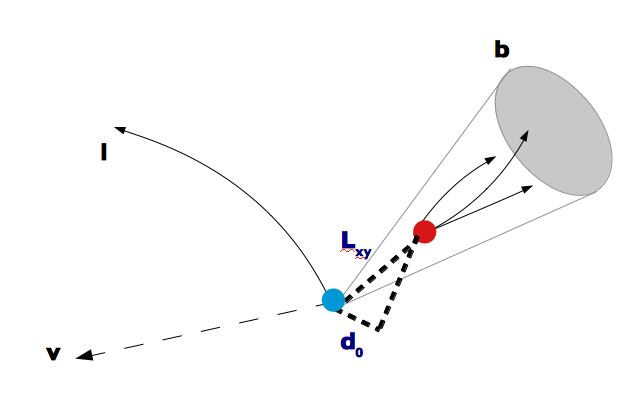
\includegraphics[width=0.6\textwidth]{img/displacedVtx}
\caption{Final state products of a $t\rightarrow Wb$ decay
with $W\rightarrow \ell\nu$.
Tracks are represented by arrows and the circles mark the primary and secondary vertices.
The \lxy\ and transverse impact parameter ($d_0$) distances which characterize the secondary vertex are
signaled by dashed lines.}
\label{fig:secvtx}
\end{center}
\end{figure}


%
%
%
\clearpage
\section{Datasets and selection}
\label{sec:datasetsandselection}

The analysis is performed using CMSSW\_5\_3\_15.

%%%
%%%
%%%
\subsection{Data analysed}
\label{subsec:data}

Collision data are analyzed using the FT\_53\_V21\_AN4 global tag while simulation samples
are processed resorting to the START53\_V23.
Data corresponds to the so-called ``Jan22 ReReco'' while
Monte-Carlo (MC) samples correspond to the official CMS Summer12\_DR53X production.

We use double lepton primary datasets for the analysis as listed in Table~\ref{tab:datasamples}. 
Data are pre-selected for ``good" luminosity sections using the 
{\small Cert\_190456-208686\_8TeV\_22Jan2013ReReco\_Collisions12\_JSON.txt}
file which is centrally provided.

\begin{table}[htp]
\centering
\caption{
Datasets used for analysis.
The primary datasets (PDs) correspond to DoubleElectron, DoubleMu, DoubleMuParked, MuEG,
SingleElectron and SingleMu.
The integrated luminosity and the run-ranges are shown for each data period.
}
\label{tab:datasamples}
\begin{tabular}{lll} 
\hline
Dataset                                & $\int \mathcal{L}$ (pb$^{-1}$)  & Run range \\
\hline\hline
{\small /PD/Run2012A-22Jan2013-v1/AOD} &  881 & {\small 190645-193621} \\
{\small /PD/Run2012B-22Jan2013-v1/AOD} & 4425 & {\small 193834-196531} \\
{\small /PD/Run2012C-22Jan2013-v1/AOD} & 7123 & {\small 198049-203742} \\
{\small /PD/Run2012D-22Jan2013-v1/AOD} & 7306 & {\small 203777-208686} \\
\hline
{\bf Total}   & {\bf 19736} & \\
\hline
\end{tabular}
\end{table}


%%%
%%%
%%%
\subsection{Simulation samples}
\label{subsec:sim}

The MC samples for various background and signal processes relevant to this analysis
are listed in Table \ref{tab:mcsamples} along with the respective
cross-sections.
For the purpose of evaluating systematic uncertainties dedicated
samples are used. These are listed in Table~\ref{tab:mcsystsamples}.
The processes have been normalized to the NLO cross sections values listed in~\cite{twiki:STDMODELXSEC8TeV}
and the \ttbar cross section has been normalized to the NNLO+NNLL
computation from~\cite{Czakon:2013goa}.
Theoretical uncertainties (QCD scales and PDFs) are taken into account
for dibosons~\cite{Campbell:2011bn}, single top~\cite{Kidonakis:2012eq} and \ttbar~\cite{Czakon:2013goa}.

All samples are generated using the \MADGRAPH~\cite{MADGRAPH}, \PYTHIA~\cite{Sjostrand:2006za} 
or \POWHEG~\cite{Alioli:2010xd}
generators and a full simulation of the CMS detector based on Geant4~\cite{Agostinelli:2002hh}.
 
\begin{table}[htp]
\caption{List of the SM dilepton MC samples used in the comparison with 8~\TeV data.
For the different processes (signal and background) considered the expected cross sections are quoted.
S12\_53 is used as an abbreviation for
Summer12\_DR53X-PU\_S10\_START53\_{V7A,V19}.
Samples marked with $\dagger$ are pre-filtered in the analysis for a
specific decay, extra parton multiplicity, etc.
}
\label{tab:mcsamples}
\begin{center}
\hspace*{-1cm}
\begin{tabular}{lll} 
\hline
Process                                & Dataset                                & $\sigma\cdot BR\cdot k$ (pb) \\
\hline\hline
\multirow{5}{*}{$W\rightarrow\ell\nu$}        
& {\small /WJetsToLNu\_TuneZ2Star\_8TeV-madgraph-tarball/S12\_53-v1 $\dagger$} &\multirow{5}{*}{36257}\\
& {\small /W1JetsToLNu\_TuneZ2Star\_8TeV-madgraph/S12\_53-v1} & \\
& {\small /W2JetsToLNu\_TuneZ2Star\_8TeV-madgraph/S12\_53-v1} & \\
& {\small /W3JetsToLNu\_TuneZ2Star\_8TeV-madgraph/S12\_53-v1} & \\
& {\small /W4JetsToLNu\_TuneZ2Star\_8TeV-madgraph/S12\_53-v1} & \\\hline
\multirow{5}{*}{$Z\rightarrow\ell\ell$}       
& {\small
  /DYJetsToLL\_M-50\_TuneZ2Star\_8TeV-madgraph-tarball/S12\_53-v1 $\dagger$} & \multirow{5}{*}{3504} \\
& {\small /DY1JetsToLL\_M-50\_TuneZ2Star\_8TeV-madgraph/S12\_53-v1}& \\
& {\small /DY2JetsToLL\_M-50\_TuneZ2Star\_8TeV-madgraph/S12\_53-v1}& \\
& {\small /DY3JetsToLL\_M-50\_TuneZ2Star\_8TeV-madgraph/S12\_53-v1}& \\
& {\small /DY4JetsToLL\_M-50\_TuneZ2Star\_8TeV-madgraph/S12\_53-v1}& \\\hline
\ttbar  & {\small  /TTJets\_MSDecays\_central\_TuneZ2star\_8TeV-madgraph-tauola/S12\_53X-v1 & 265\\\hline
\ttbar+V                       & {\small /TTWJets\_8TeV-madgraph/S12\_53-v1}                                      & 0.232\\
                               & {\small /TTZJets\_8TeV-madgraph\_v2/S12\_53-v1}                                  & 0.208\\\hline
\multirow{6}{*}{Single top}    & {\small /Tbar\_tW-channel-DR\_TuneZ2star\_8TeV-powheg-tauola/S12\_53-v1 ($\bar{t}$)} & 11.2\\
                               & {\small /T\_tW-channel-DR\_TuneZ2star\_8TeV-powheg-tauola/S12\_53-v1 ($t$)}          & 11.2\\
                               & {\small /Tbar\_t-channel\_TuneZ2star\_8TeV-powheg-tauola/S12\_53-v1 ($\bar{t}$)}     & 55.5\\
                               & {\small /T\_t-channel\_TuneZ2star\_8TeV-powheg-tauola/S12\_53-v1 ($t$)}              & 30.0 \\
                               & {\small /Tbar\_s-channel\_TuneZ2star\_8TeV-powheg-tauola/S12\_53-v1 ($\bar{t}$)}     & 3.89 \\
                               & {\small /T\_s-channel\_TuneZ2star\_8TeV-powheg-tauola/S12\_53-v1 ($t$)}              & 1.76 \\\hline
\multirow{3}{*}{Dibosons (VV)} & {\small /WZJetsTo3LNu\_TuneZ2\_8TeV-madgraph-tauola/S12\_53-v1}                      & 1.057\\
                               & {\small /WWJetsTo2L2Nu\_TuneZ2star\_8TeV-madgraph-tauola/S12\_53-v1}                 & 5.71\\
                               & {\small /ZZJetsTo2L2Nu\_TuneZ2star\_8TeV-madgraph-tauola/S12\_53-v3}                 & 0.3198 \\
\hline
\end{tabular}
\end{center}
\end{table}

\begin{table}[htp]
\caption{List of the \ttbar systematic MC samples used in the analysis.
The abbreviations are similar to the ones used for
Table~\ref{tab:mcsamples}.
ME-PS (UE) stands for matrix-element to parton-shower threshold
(underlying event).
}
\label{tab:mcsystsamples}
\begin{center}
\hspace*{-0.5cm}
\begin{tabular}{ll} 
\hline
Systematic & Dataset  \\
\hline\hline
\multirow{2}{*}{$Q^2=\mu_R^2=\mu_F^2$}        
& {\small /TTJets\_MSDecays\_scaledown\_TuneZ2star\_8TeV-madgraph-tauola//S12\_53-v1}\\
& {\small /TTJets\_MSDecays\_scaleup\_TuneZ2star\_8TeV-madgraph-tauola//S12\_53-v1 }\\\hline
\multirow{2}{*}{ME-PS}        
& {\small /TTJets\_MSDecays\_matchingdown\_TuneZ2star\_8TeV-madgraph-tauola/S12\_53-v1}\\
& {\small /TTJets\_MSDecays\_matchingup\_TuneZ2star\_8TeV-madgraph-tauola/S12\_53-v1 }\\\hline
\multirow{8}{*}{UE,CR}        
& {\small /TTJets\_FullLeptMGDecays\_TuneP11\_8TeV-madgraph-tauola/S12\_53-v1 }\\
& {\small /TTJets\_FullLeptMGDecays\_TuneP11mpiHi\_8TeV-madgraph-tauola/S12\_53-v1}\\
& {\small /TTJets\_FullLeptMGDecays\_TuneP11TeV\_8TeV-madgraph-tauola/S12\_53-v1}\\
& {\small /TTJets\_FullLeptMGDecays\_TuneP11noCR\_8TeV-madgraph-tauola/S12\_53-v1}\\
& {\small /TTJets\_SemiLeptMGDecays\_TuneP11\_8TeV-madgraph-tauola/S12\_53-v1 }\\
& {\small /TTJets\_SemiLeptMGDecays\_TuneP11mpiHi\_8TeV-madgraph-tauola/S12\_53-v1}\\
& {\small /TTJets\_SemiLeptMGDecays\_TuneP11TeV\_8TeV-madgraph-tauola/S12\_53-v1}\\
& {\small /TTJets\_SemiLeptMGDecays\_TuneP11noCR\_8TeV-madgraph-tauola/S12\_53-v1}\\\hline
\multirow{2}{*}{Hadronization, Signal}&
{\small /TT\_CT10\_TuneZ2star\_8TeV-powheg-tauola/S12\_53-v2}\\
&{\small /TT\_CT10\_AUET2\_8TeV-powheg-tauola/S12\_53-v1}\\
\hline
\multirow{6}{*}{Mass} 
& {\small /TTJets\_MSDecays\_mass166\_5\_TuneZ2star\_8TeV-madgraph-tauola/S12\_53-v1}\\
& {\small /TTJets\_MSDecays\_mass169\_5\_TuneZ2star\_8TeV-madgraph-tauola/S12\_53-v1}\\
& {\small /TTJets\_MSDecays\_mass171\_5\_TuneZ2star\_8TeV-madgraph-tauola/S12\_53-v1}\\
& {\small /TTJets\_MSDecays\_mass173\_5\_TuneZ2star\_8TeV-madgraph-tauola/S12\_53-v1}\\
& {\small /TTJets\_MSDecays\_mass175\_5\_TuneZ2star\_8TeV-madgraph-tauola/S12\_53-v1}\\
& {\small /TTJets\_MSDecays\_mass178\_5\_TuneZ2star\_8TeV-madgraph-tauola/S12\_53-v1}\\
\hline
\end{tabular}
\end{center}
\end{table}



%%
%%
%%
\subsection{Corrections applied to the simulation}
\label{subsec:simcorrections}

The pileup distribution in the MC is re-weighted to match the one
estimated in data.
After applying the re-weighting procedure the vertex multiplicity
distribution is used to evaluate the expected level of agreement.
Figure~\ref{fig:vtxmult} shows the resulting vertex multiplicity
distribution observed after the selection of two good leptons in the
event.
The lepton selection applied will detailed below.

\begin{figure}[htp] 
\centering
\subfloat[][]{\includegraphics[width=0.48\textwidth]{img/ll_nvertices}}
\subfloat[][]{\includegraphics[width=0.48\textwidth]{img/l_nvertices}}
\caption{ 
Vertex multiplicity distribution in the 2012 dataset for the (a) dilepton 
and (b) single lepton channels compared to the simulation  after the reweighing procedure.
MC is normalized by the cross section and the integrated luminosity.
}
\label{fig:vtxmult}
\end{figure}


%%%
%%%
%%%
\subsection{Event selection}
\label{subsec:evsel}

The event selection is briefly summarized in this section.
Table~\ref{tab:datatriggers} reports the triggers used in the
analysis.
The dilepton ($ee$, $\mu\mu$ or $e\mu$) and the single lepton ($e$, $\mu$) channels
are determined by both
the trigger and the offline reconstructed final state. Double counting
of the events is removed by giving requiring the trigger type to be matched
to the final state being observed
and giving priority to $e\mu$ over $\mu\mu$ over $ee$ events over $\mu$ over $e$, sequentially. 

\begin{table}[!htp]
\centering
\caption{
Triggers used for the analysis. If more than one trigger is listed per
final state, a logical OR is used to acquire the data.
}
\label{tab:datatriggers}
\begin{tabular}{ll} \hline
 Dataset          & Trigger paths \\
\hline\hline
$ee$ & {\small Ele17\_CaloIdT\_CaloIsoVL\_TrkIdVL\_TrkIsoVL\_Ele8\_CaloIdT\_CaloIsoVL\_TrkIdVL\_TrkIsoVL }\\
\hline
\multirow{2}{*}{$\mu\mu$} & {\small Mu17\_Mu8}\\
                          & {\small Mu17\_TkMu8}\\
\hline
\multirow{2}{*}{$e\mu$}   & {\small Mu8\_Ele17\_CaloIdT\_CaloIsoVL\_TrkIdVL\_TrkIsoVL} \\
                          & {\small Mu17\_Ele8\_CaloIdT\_CaloIsoVL\_TrkIdVL\_TrkIsoVL} \\
\hline
$e$ & {\small Ele27\_WP80} \\
\hline
$\mu$ & {\small IsoMu24\_eta2p1} \\
\hline
\end{tabular}
\end{table}

The offline selection is as follows:

\begin{itemize}

\item at least one charged lepton is required in the event.
  Electron identification is based on a multivariate discriminator and we
  require it to be $>$0.5. For muons we make use of the Tight
  identification criteria. PF-based isolation is used in both
  cases. Electrons are required to have a relative isolation $<$0.15
  corrected using an effective isolation area and the event-by-event
  estimate of the energy density flow due to pileup and underlying
  event, \ie $\rho$. Muons are required to have a relative isolation
  $<$0.12 corrected using tracks which point to pileup vertices in the
  event.
  For single lepton events we require one lepton with \pt$>$30\GeV and $\lvert\eta\rvert<$2.5
  in the e channel or \pt$>$26\GeV and $\lvert\eta\rvert<$2.1 in the $\mu$ channel.
  For dilepton events we require two leptons with \pt$>$20\GeV, $\lvert\eta\rvert<$2.5
  and $M_{\ell\ell}>$12\GeV. In the case of ee or $\mu\mu$ channels, 
  events with $\vert M_{\ell\ell}-M_\cPZ\vert<15\GeV$ are rejected.

\item at least two (four) AK5 PF-reconstructed jets with charged hadron
  subtraction corrections and with \pt$>$20\GeV and $\lvert\eta\rvert<$2.5
  are required in dilepton (single lepton) events. The loose PF-jet id is applied
  as well as jet energy corrections. For the simulated samples we smear further
  the jet energy resolution. The smearing procedure is described in
  more detail in~\cite{twiki:JER}.

\item for same-flavour dilepton events we require further that \MET$>$40\GeV
  The missing transverse energy is computed from the absolute value of the \pt balance of all PF candidates.

\end{itemize}


The trigger and lepton selection efficiencies are determined from data
using a tag and probe method. The scale factor, with respect to the
efficiencies expected from simulation, is then used to re-weigh the simulated
events with two prompt leptons.
The Muon and EGamma POG recommended values are used~\cite{twiki:EGeff,twiki:MUeff}.


%%
%%
%%
\clearpage
\section{Background control}
\label{sec:bckgctrl}

Coming soon.

%%
%%
%%
\clearpage
\section{Event yields and control distributions}
\label{sec:evyields}

Coming soon.

%%
%%
%%
\clearpage
\section{Truth and Lies about Beauty and Charm: using top quark pair events as a spectroscope to
control the modelling of fragmentation and hadronization of $\cPqb$ jets}
\label{sec:truthlies}

We make use of the charged particle flow candidates associated to the two jets which rank highest in the CSV discriminator.
Particle flow classifies the charged candidates as electrons, muons or charged hadrons.
For the latter case we assign a mass hypothesis ($\pi^\pm$ or K$^\pm$) depending on the combination being tested.
Three charmed mesons are considered for our study:

\begin{description}
\item[$D^0$ candidates] - are chosen due to the large branching ratio, \ie 
${\rm BR}(B^+\rightarrow D^0+X)\times{\rm BR}(D^0\rightarrow K^+\pi^-)\approx 79\times3.9\%=3.1\%$~\cite{Beringer:1900zz}.
We reconstruct $D^0$ candidates assuming the $K^+\pi^-$ decay channel and using all the permutations
made of up to 5 leading-\pt charged hadrons. 
The purity of this selection is enhanced by finding a lepton with the same charge of the 
kaon assignment in a given permutation;
\item[$D^\pm$ candidates] - are chosen given they are expected to be the second most probable charmed mesons to be found after a B-hadron decay, \ie
${\rm BR}(B^+\rightarrow D^++X)\times{\rm BR}(D^+\rightarrow K^+2\pi^-)\approx 9.9\times9.1\%=0.9\%$~\cite{Beringer:1900zz}. The candidates are reconstructed using triples of charged hadrons in which two have the same electric charge, opposite to that of the third charge hadron. All permutations made of up to 5 leading-\pt charged hadrons are tried.
\item[$J/\psi$ candidates] - are chosen owing to the expected high purity selection, stemming from the 
distinct final state containing two op. sign, same flavour leptons (e or $\mu$).
The reconstruction requires two leptons associated to the jet, in the conditions mentioned before;
\end{description} 

Figure~\ref{fig:charmedresonances} compares the data to simulation-based expectations for the invariant mass distribution
of the different charmed meson candidates. The agreement is overall good in the production rate and shape of the distributions.
The major discrepancies are observed 
for the $J/\psi\rightarrow \mu^+\mu^-$ spectrum in data which may be related to 
residual PF muon energy calibration but also to the background modelling in simulation
and for the region of the $D^\pm$ peak where an overall 20\% excess in data is observed.

\begin{figure}[htp] 
\centering
\subfloat[][]{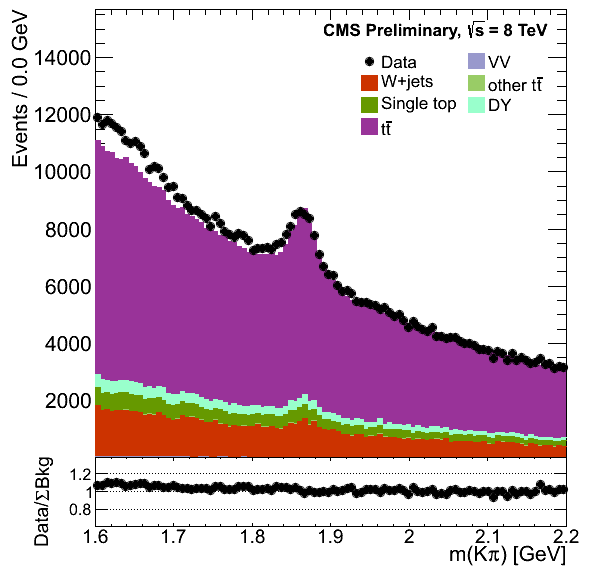
\includegraphics[width=0.48\textwidth]{img/charm/D0Incl3Trk.png}}
\subfloat[][]{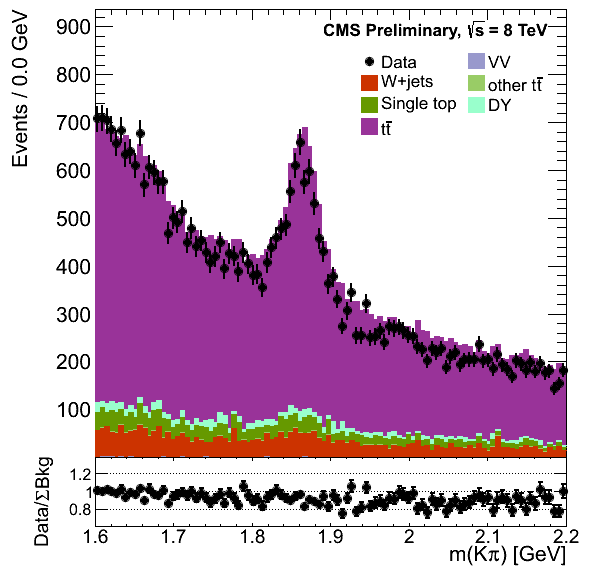
\includegraphics[width=0.48\textwidth]{img/charm/D0lep.png}}\\
\subfloat[][]{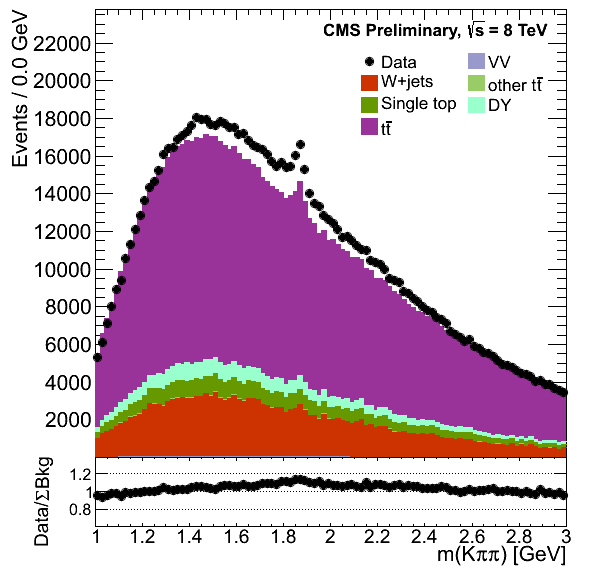
\includegraphics[width=0.48\textwidth]{img/charm/DpmZO.png}}
\subfloat[][]{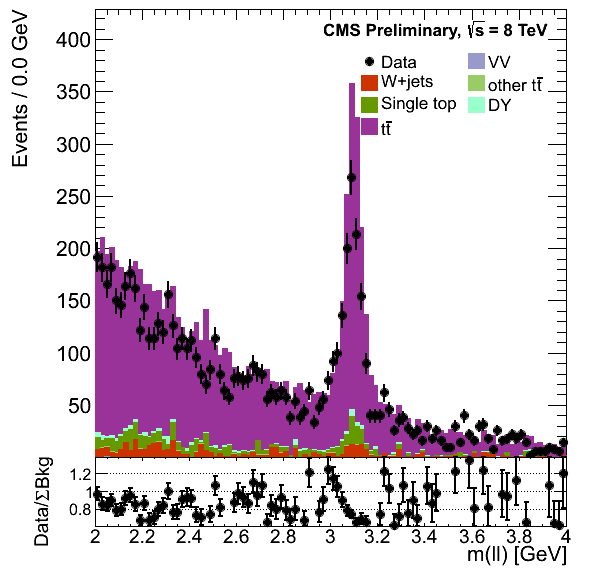
\includegraphics[width=0.48\textwidth]{img/charm/JPsi.png}}
\caption{ 
Invariant mass distributions of charmed meson candidates in \ttbar events:
(a) $D^0$, (b) $D^0$ with soft lepton tag, (c) $D^\pm$ and (d) $J/\psi$.
The expectations for the different processes are shown stacked and the data is shown as marker points.
The bottom panels show the ratio of data to the total expectations.
}
\label{fig:charmedresonances}
\end{figure}

In order to characterize the kinematic properties of these charmed resonances we make use of
the sPlot technique~\cite{2005NIMPA.555..356P}.
The invariant mass distributions are fitted to determine the contribution from signal and background.
In the fit both the parameters of the distributions as well as the yields of the signal and background  are determined.
The result is then used to unfold the contributions of the different sources to the distribution of a given variable
without using any a priori knowledge on it.
By applying this technique on both data and MC we are able to compare the results with different models.
Notice that the variable being unfolded must be, in first approximation,
uncorrelated with the mass distribution, otherwise extra correction factors would need to be applied.
Also notice, that to obtain a fully unfolded distribution which could be compared at generator level,
e.g. with the \textsc{rivet} framework~\cite{Buckley:2010ar}, 
an extra step would be needed of deriving possible
extra corrections between the unfolded sPlot distribution and the truth distribution in simulation.
For our purposes having a consistent setup in data and MC is sufficient. 
Moreover we don't expect these corrections
to be significant given we'll be using mostly tracker-reconstructed quantities. 

The signal is modeled with a Crystal-Ball function and the background with an exponential function.
An extended unbinned likelihood fit is used to extract the signal and background yields 
and fix the parameters of the probability distribution functions.
The fit is implemented in \textsc{roofit}~\cite{2003physics...6116V}.
Table~\ref{tab:charmfit} summarizes the average mass, 
width and the signal-to-background (S/B) extracted in data and
in simulation, for the different resonances.


\begin{table}[!htp]
\centering
\caption{Average mass and width obtained from the fit to the invariant mass distributions 
in data and different simulations. The signal-to-background ratio obtained (S/B) is also shown.
The uncertainties are of statistical nature.
}
\label{tab:charmfit}
\begin{tabular}{lllccc} \hline
Candidate & \multicolumn{2}{l}{Dataset} & Mass (\GeV) & Width (\GeV) & S/B \\
\hline\hline
\multirow{5}{*}{$D^0$} 
& \multicolumn{2}{l}{Data} & 1.8636$\pm$0.0009 & 0.020$\pm$0.001 & 0.114$\pm$0.006\\ 
\cline{2-6}
& \multirow{4}{*}{MC} & MG+PY+Z2$^*$ & 1.866$\pm$0.001   & 0.019$\pm$0.002   & 0.115$\pm$0.011\\ 
&                     & MG+PY+P11    & 1.8669$\pm$0.0006 & 0.0180$\pm$0.0007 & 0.113$\pm$0.004\\ 
&                     & PW+PY+Z2$^*$ & 1.8655$\pm$0.0006 & 0.0194$\pm$0.0006 & 0.116$\pm$0.004\\ 
&                     & PW+HW+AUET2 & 1.8653$\pm$0.0005 & 0.0191$\pm$0.0005 & 0.145$\pm$0.004\\ 
\hline
\multirow{5}{*}{$D^0$ (soft-lepton tag)} 
& \multicolumn{2}{l}{Data} & & & \\ 
\cline{2-6}
& \multirow{4}{*}{MC} & MG+PY+Z2$^*$ & & \\ 
&                     & MG+PY+P11 & & \\ 
&                     & PW+PY+Z2$^*$ & & \\ 
&                     & PW+HW+AUET2 & & \\ 
\hline
\multirow{5}{*}{$D^\pm$} 
& \multicolumn{2}{l}{Data} & & & \\ 
\cline{2-6}
& \multirow{4}{*}{MC} & MG+PY+Z2$^*$ & & \\ 
&                     & MG+PY+P11 & & \\ 
&                     & PW+PY+Z2$^*$ & & \\ 
&                     & PW+HW+AUET2 & & \\ 
\hline
\multirow{5}{*}{$J/\psi$} 
& \multicolumn{2}{l}{Data} & & & \\ 
\cline{2-6}
& \multirow{4}{*}{MC} & MG+PY+Z2$^*$ & & \\ 
&                     & MG+PY+P11 & & \\ 
&                     & PW+PY+Z2$^*$ & & \\ 
&                     & PW+HW+AUET2 & & \\ 
\hline
\end{tabular}
\end{table}

The mass fit described above is performed in different \pt and $\eta$
ranges. Given there is a correlation between the invariant mass resolution and these
two variables we adopt this technique to measure the different $\pt$ and $\eta$
production cross sections for the charmed meson candidates.
The ranges are chosen such that the mean fitted does not deviate from the central value
quoted in Table~\ref{tab:charmfit} by more than 1$\sigma$.

Figures~\ref{fig:charmptdiff} and~\ref{fig:charmetadiff}
shows the results obtained for the $\pt$ and $\eta$.
Different models are compared with the data.
Overall data tends to agree with the prediction obtained with the \MADGRAPH+\PYTHIA+Z2$^*$ setup.
After changing the matrix-element generator
we expect differences in the kinematics of the mesons, in particular in $\eta$.
The result is not unexpected given \MADGRAPH is a LO generator including up to three partons at matrix-element level,
and \POWHEG is a NLO generator including up to one extra parton at matrix-element level.
Data tends to agree better with \MADGRAPH,
but, if \HERWIG is used instead as the hadronizer, the agreement with \POWHEG improves.
The variation of the tune for the same matrix-element+parton-shower choice (\MADGRAPH and \PYTHIA)
induces some differences in the spectra as well, with data being closer to Z2$^*$.

\begin{figure}[htp] 
\centering
\subfloat[][]{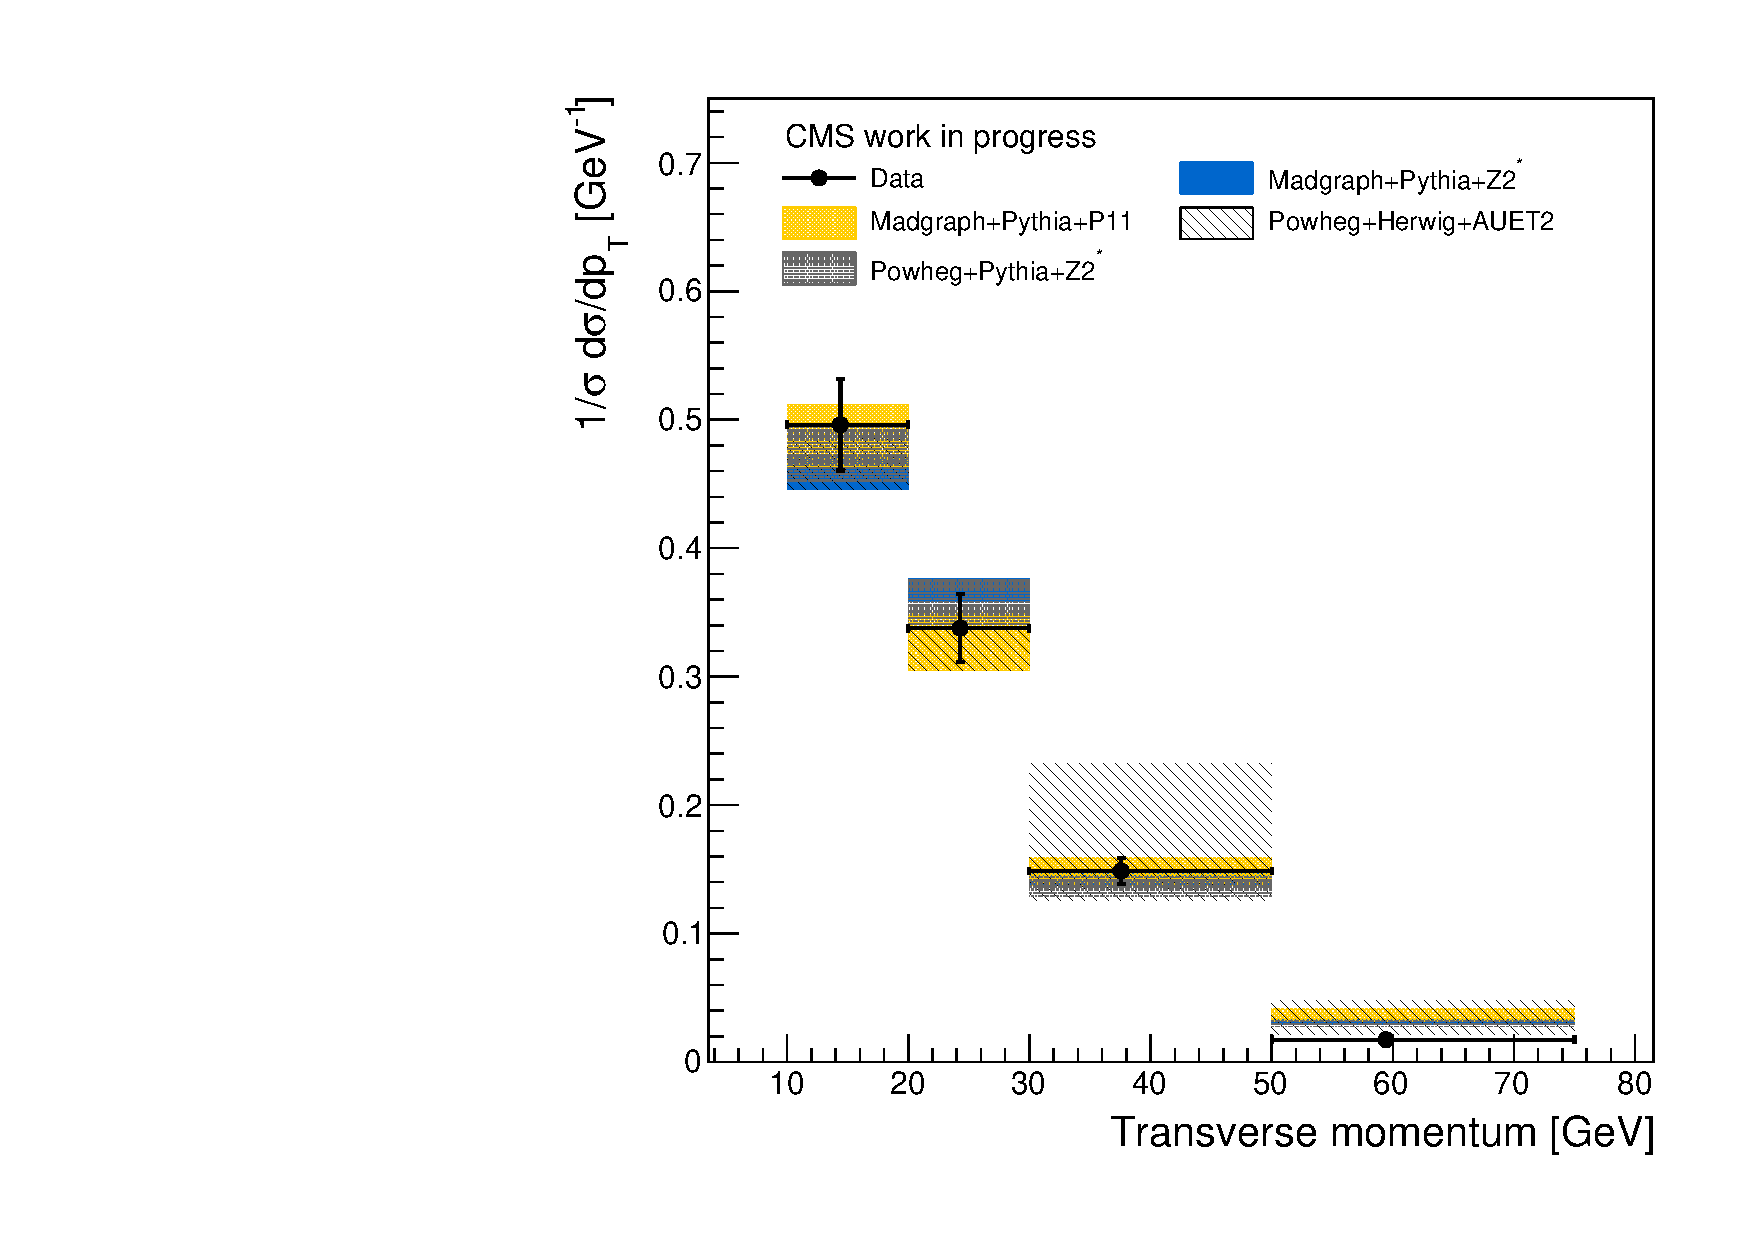
\includegraphics[width=0.48\textwidth]{img/charm/D0Incl3Trk_diffpt}}
\subfloat[][]{\includegraphics[width=0.48\textwidth]{img/charm/D0lep_diffpt}}\\
\subfloat[][]{\includegraphics[width=0.48\textwidth]{img/charm/DpmZO_diffpt}}
\subfloat[][]{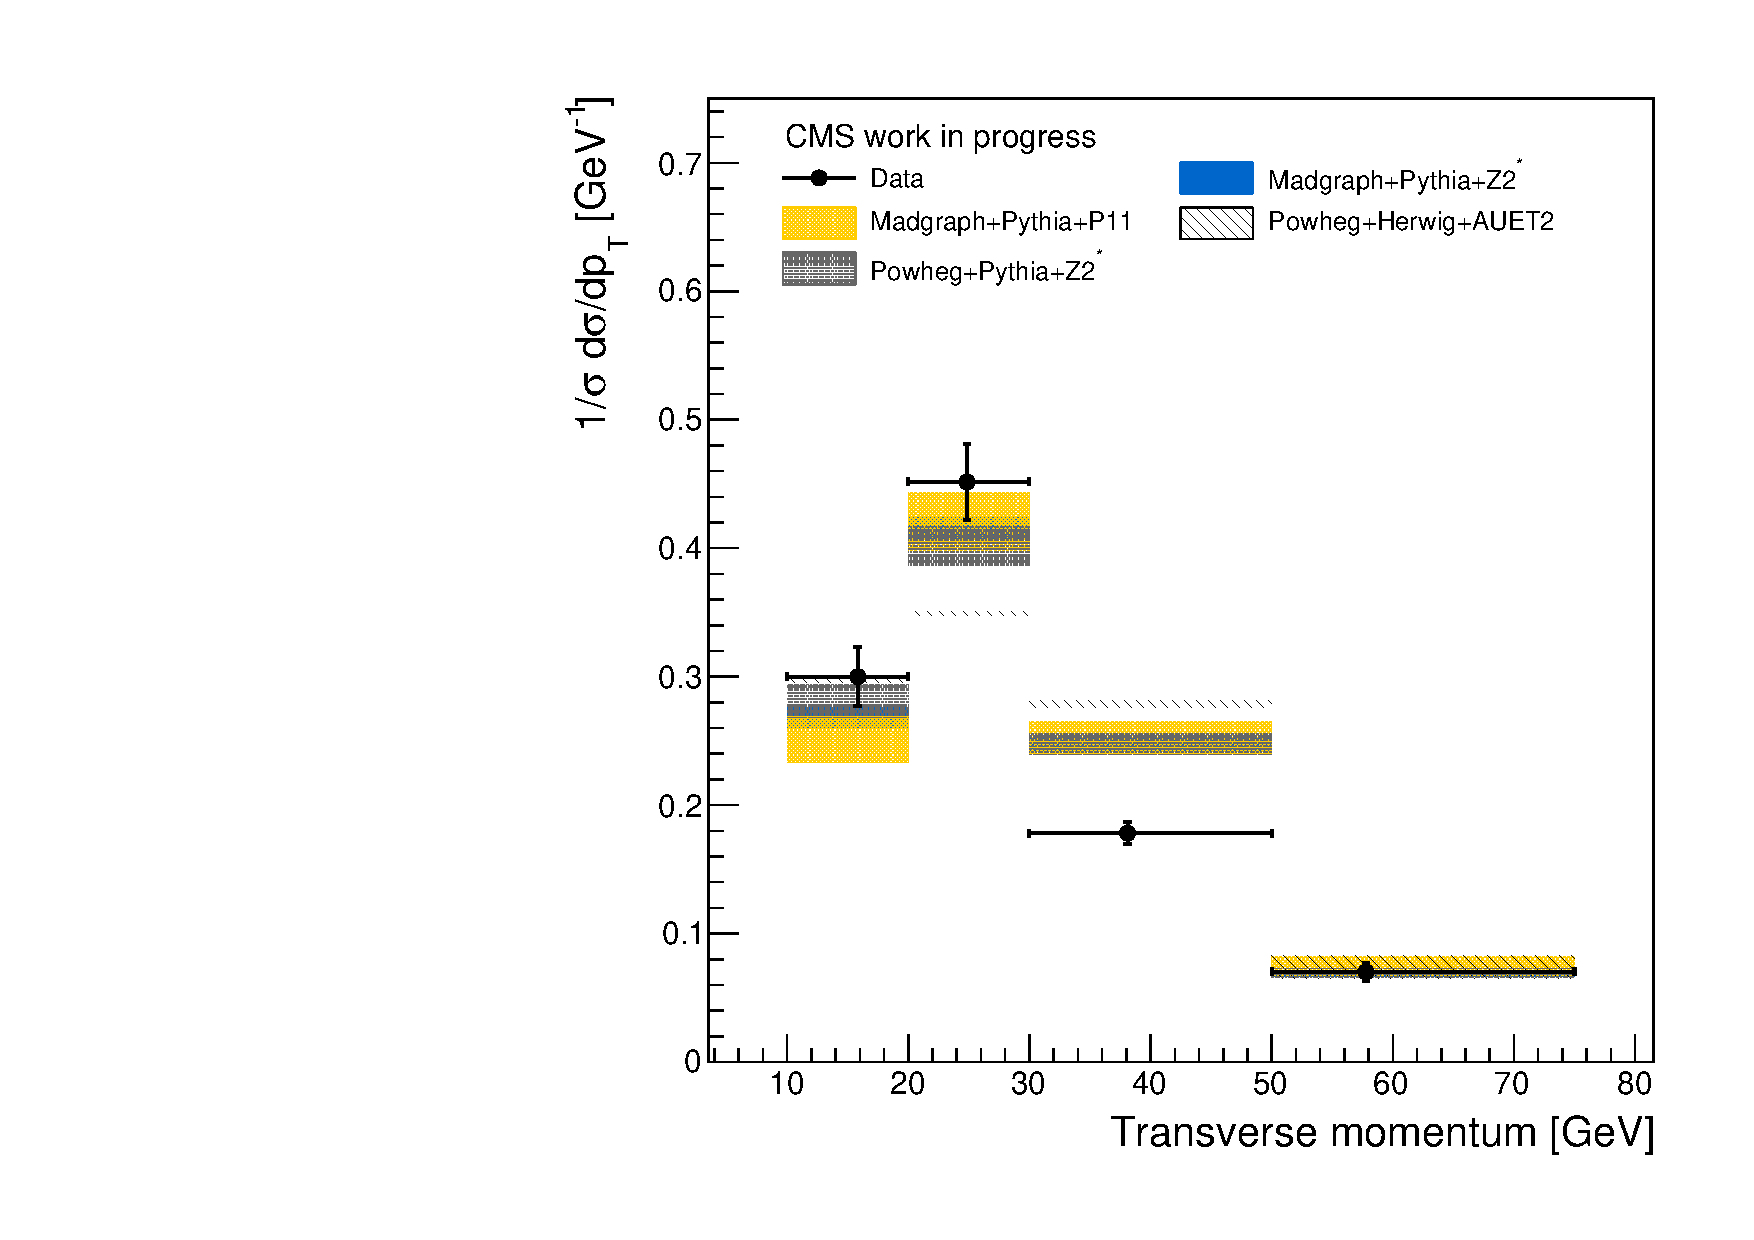
\includegraphics[width=0.48\textwidth]{img/charm/JPsi_diffpt}}
\caption{ 
Normalized differential production cross section of charmed meson candidates in \ttbar events,
as function of \pt:
(a) $D^0$, (b) $D^0$ with soft lepton tag, (c) $D^\pm$ and (d) $J/\psi$.
The expectations for different \ttbar models are shown as shaded bands
while the data is shown as marker points.
Bin-center corrections have been applied to both data and MC
}
\label{fig:charmptdiff}
\end{figure}

\begin{figure}[htp] 
\centering
\subfloat[][]{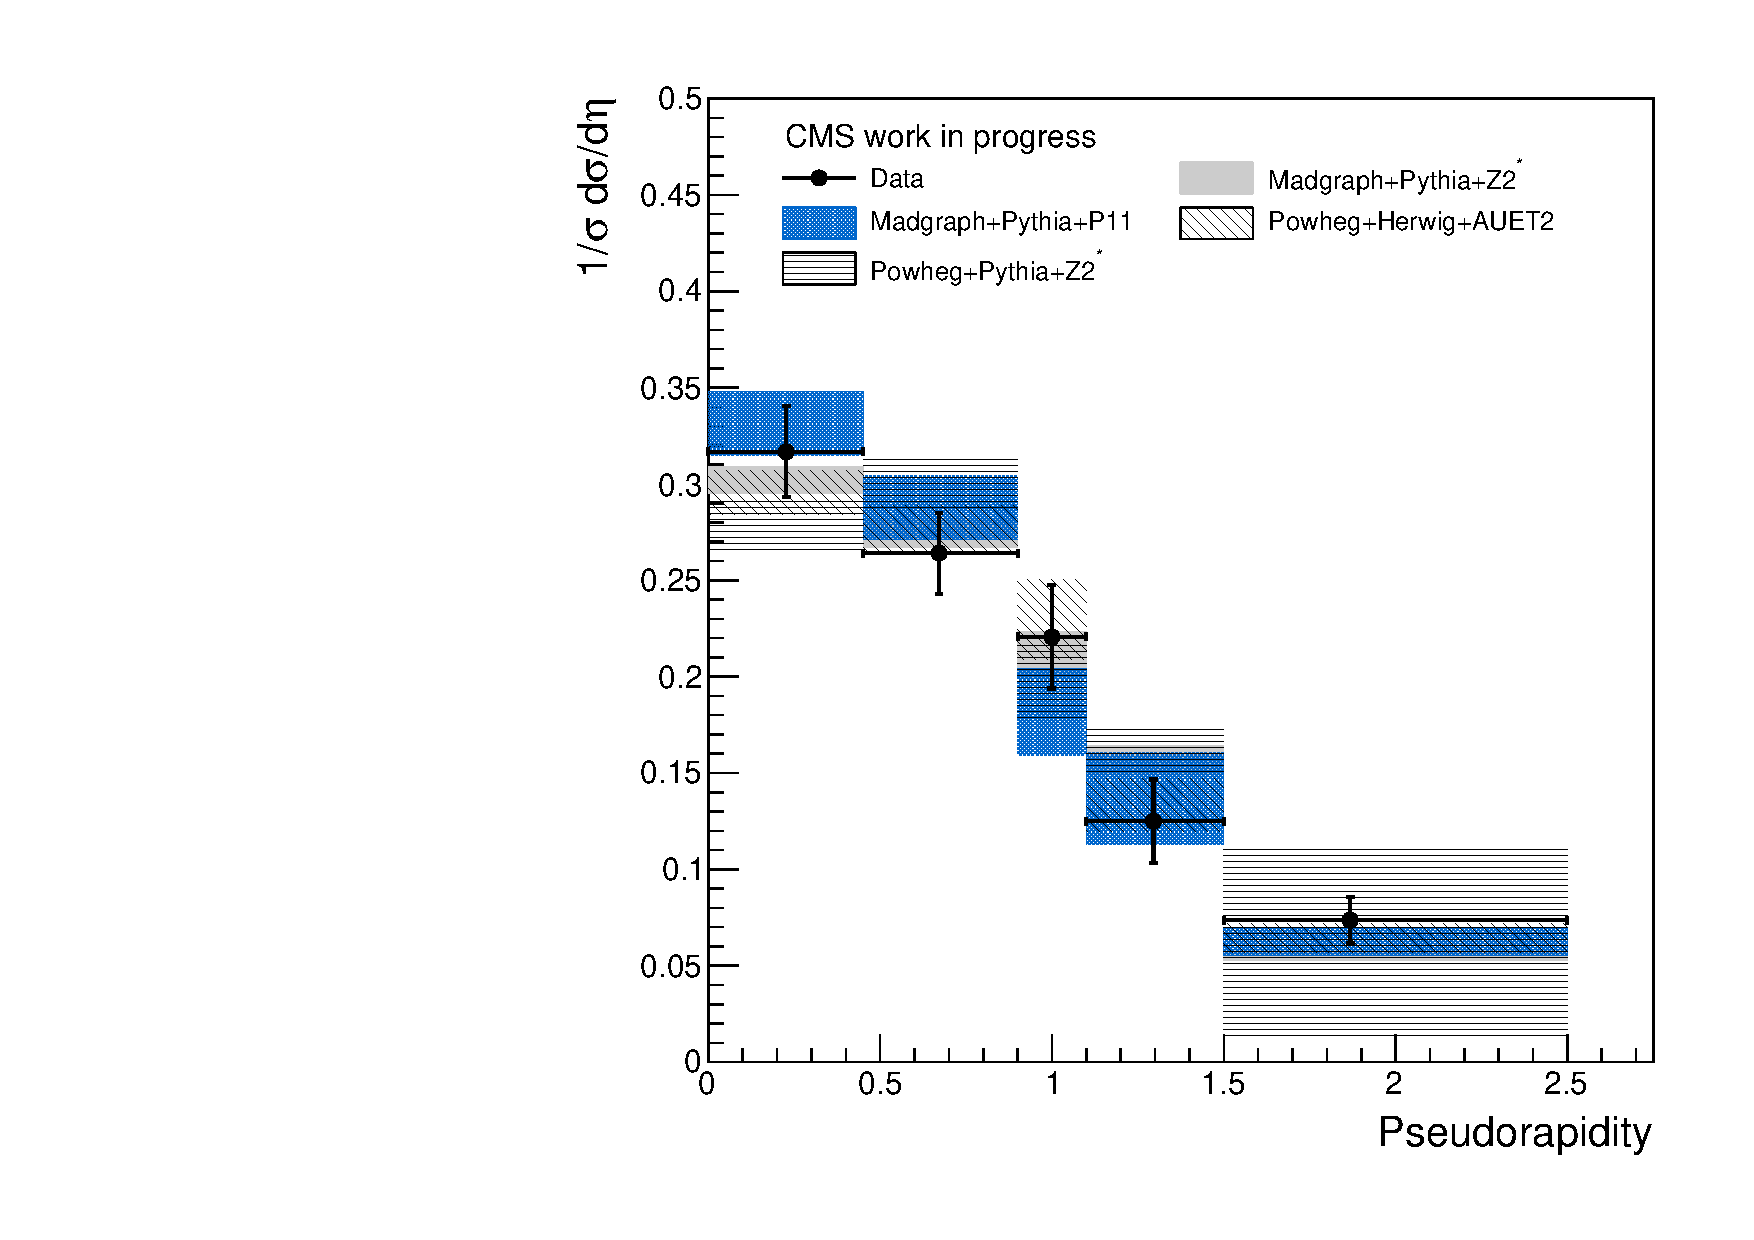
\includegraphics[width=0.48\textwidth]{img/charm/D0Incl3Trk_diffeta}}
\subfloat[][]{\includegraphics[width=0.48\textwidth]{img/charm/D0lep_diffeta}}\\
\subfloat[][]{\includegraphics[width=0.48\textwidth]{img/charm/DpmZO_diffeta}}
\subfloat[][]{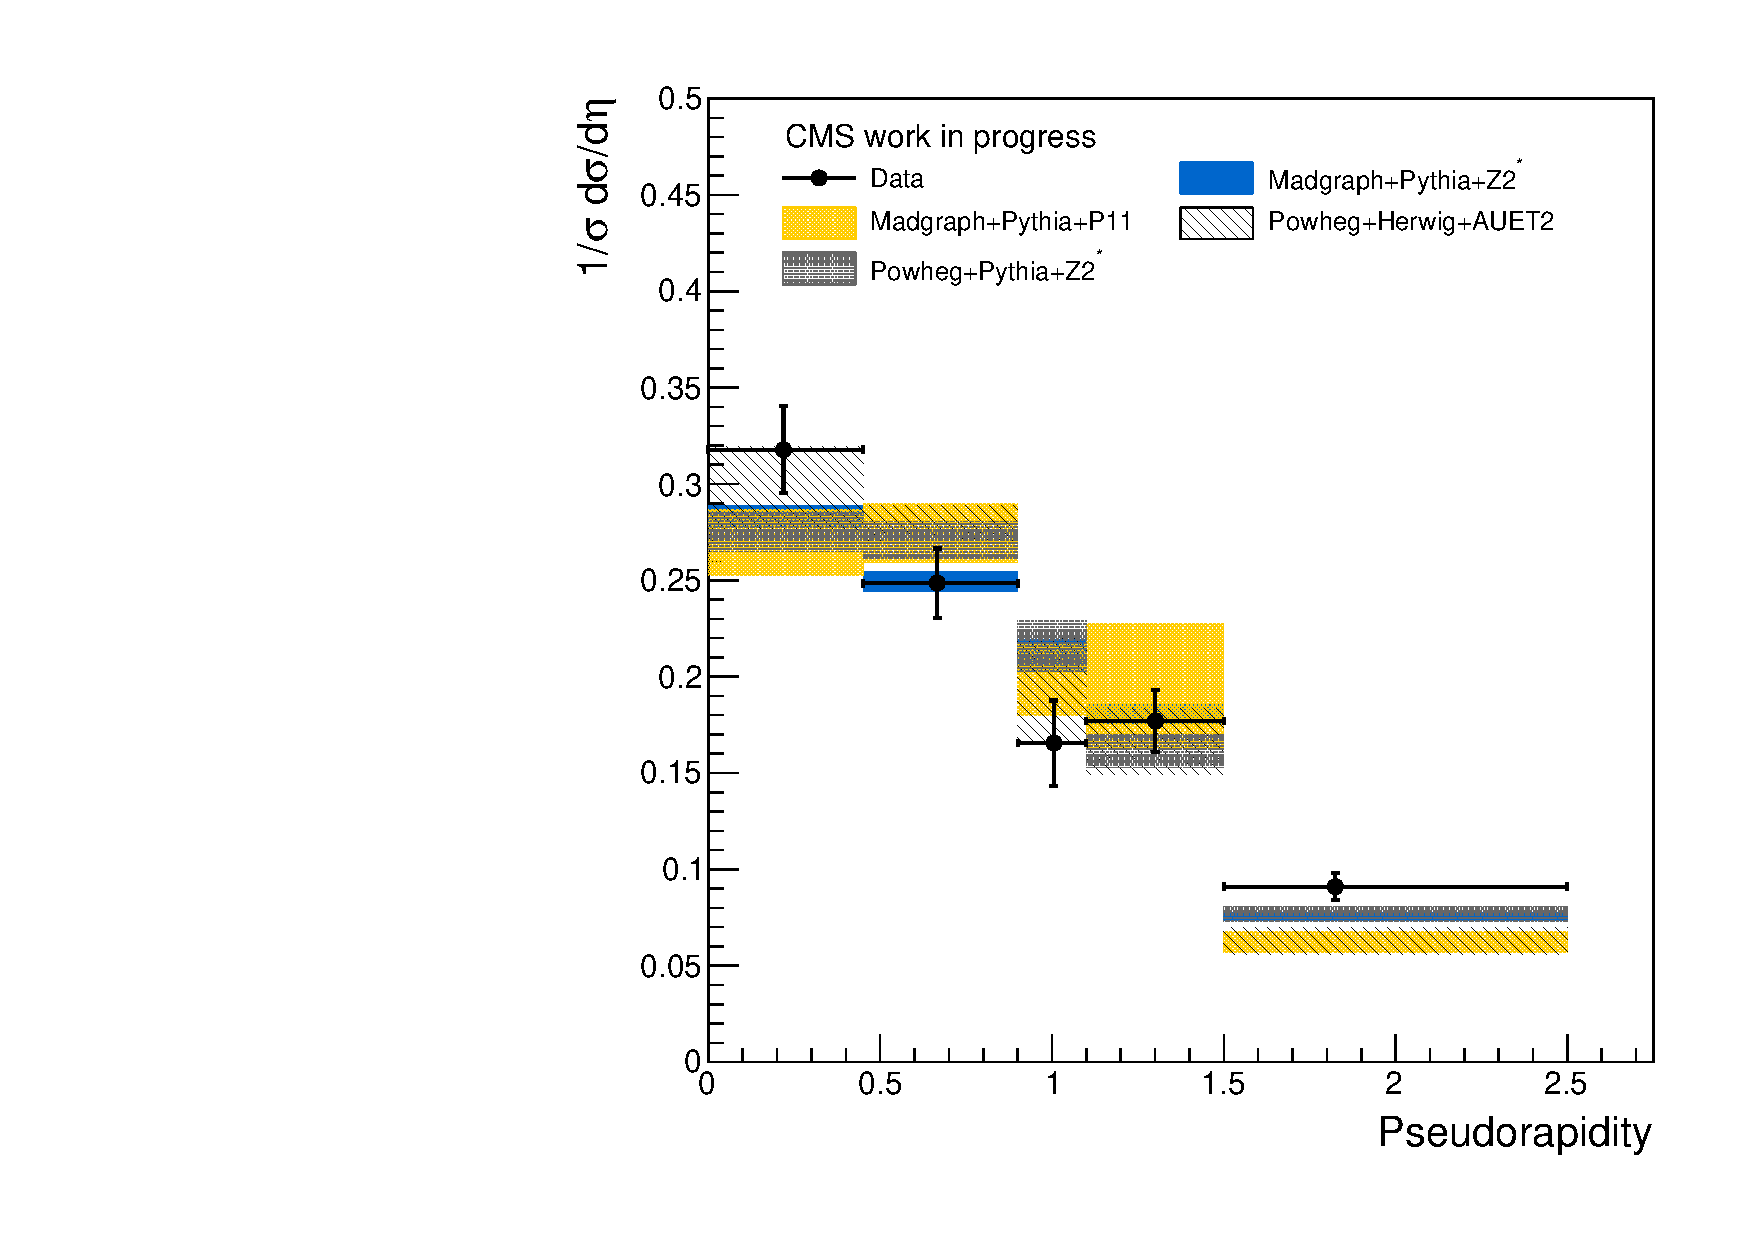
\includegraphics[width=0.48\textwidth]{img/charm/JPsi_diffeta}}
\caption{ 
Normalized differential production cross sections of charmed meson candidates in \ttbar events,
as function of $\eta$:
(a) $D^0$, (b) $D^0$ with soft lepton tag, (c) $D^\pm$ and (d) $J/\psi$.
The expectations for different \ttbar models are shown as shaded bands
while the data is shown as marker points.
Bin-center corrections have been applied to both data and MC.
}
\label{fig:charmetadiff}
\end{figure}

Using the inclusive $\pt$ and $\eta$ spectra we unfold different kinematics variables
of the charmed mesons which are, in first approximation uncorrelated to the reconstructed mass of the candidates,
given the variables are defined relatively to jet quantities:

\begin{description}

\item[Ratios to jet kinematics] - the ratios of the momentum, transverse momentum or longitudinal momentum of the charmed meson, with respect to the jet's momentum, transverse momentum or longitudinal momentum are quantities which are sensitive to the jet energy scale. We denote these ratios as $R_p$, $R_{p_{\rm T}}$ and $R_{p_{\rm z}}$ respectively;

\item[\ptrel] - the relative momentum of the charmed meson with respect to the jet axis is expected to be less sensitive to the jet energy scale and it is defined as:

\begin{equation}
p_{\rm T}^{\rm rel}=\vert\vec{p}-\frac{\vec{p}\cdot\vec{p_{\rm jet}}}{\vert\vec{p}_{\rm jet}\vert^2}\vec{p_{\rm jet}}\vert~,
\label{eq:ptrel}
\end{equation}

where $\vec{p}$ and $\vec{p}_{\rm jet}$ are correspondingly the charmed meson and the jet transverse momentum.

\item[Ratios to charged component in jet] - the ratios of the transverse momentum or longitudinal momentum of the charmed meson, with respect to the sum of all the jet's charged particle flow candidates' transverse momentum or longitudinal momentum are quantities which are practically insensitive to the jet energy scale. We denote these ratios as $R_{p_{\rm T}}^{\rm ch}$ and $R_{p_{\rm z}}^{\rm ch}$ respectively;

\item[Angular distance to the jet] - the $\Delta R$ distance is practicaly insensitive to the jet energy scale.

\item
\end{description}

The unfolded distributions are shown in Figures~\ref{fig:d0kinematics},
\ref{fig:d0lepkinematics}, \ref{fig:dpmkinematics} and \ref{fig:jpsikinematics}
for the $D^0$, $D^0$ with soft lepton tag, $D^\pm$ and $J/\psi$ candidates.

\begin{figure}[htp] 
\centering
\subfloat[][]{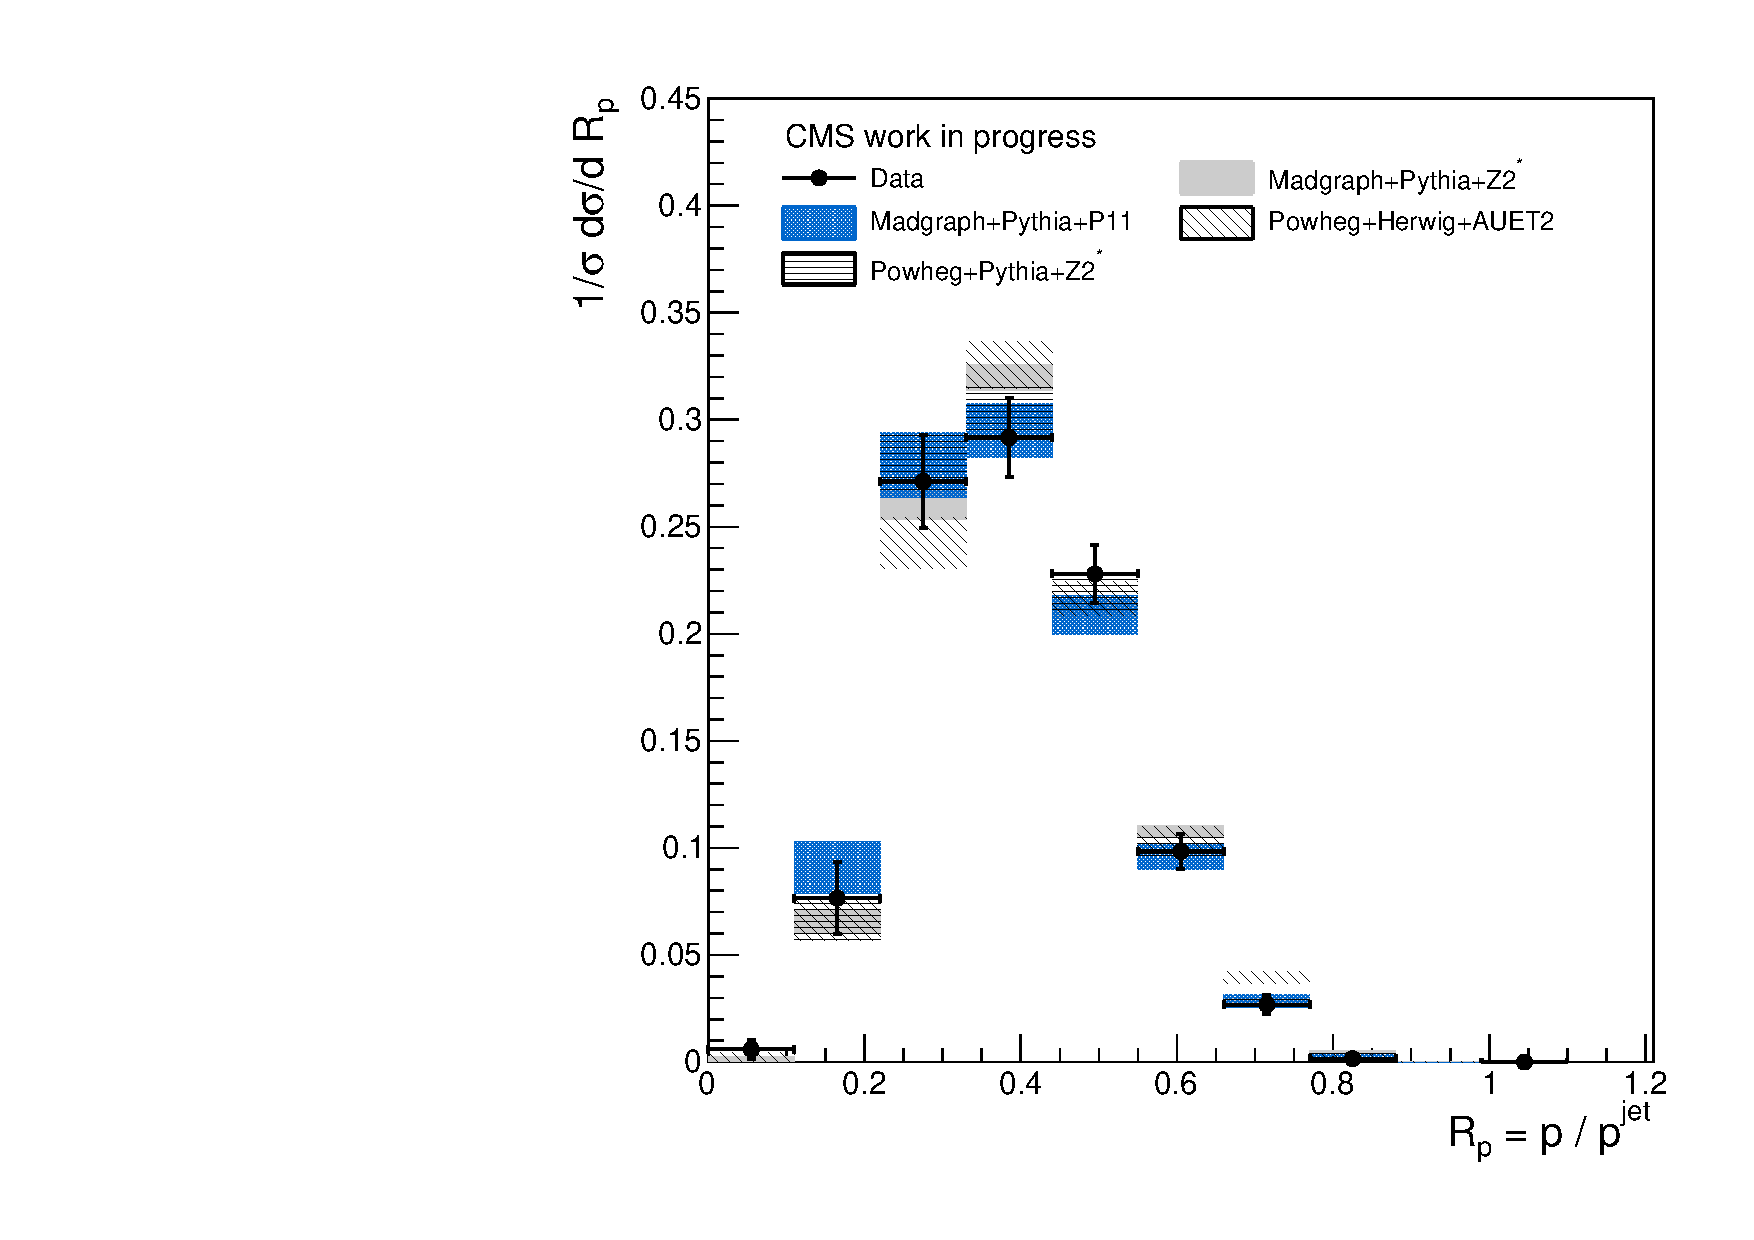
\includegraphics[width=0.32\textwidth]{img/charm/D0Incl3Trk_pfrac}}
\subfloat[][]{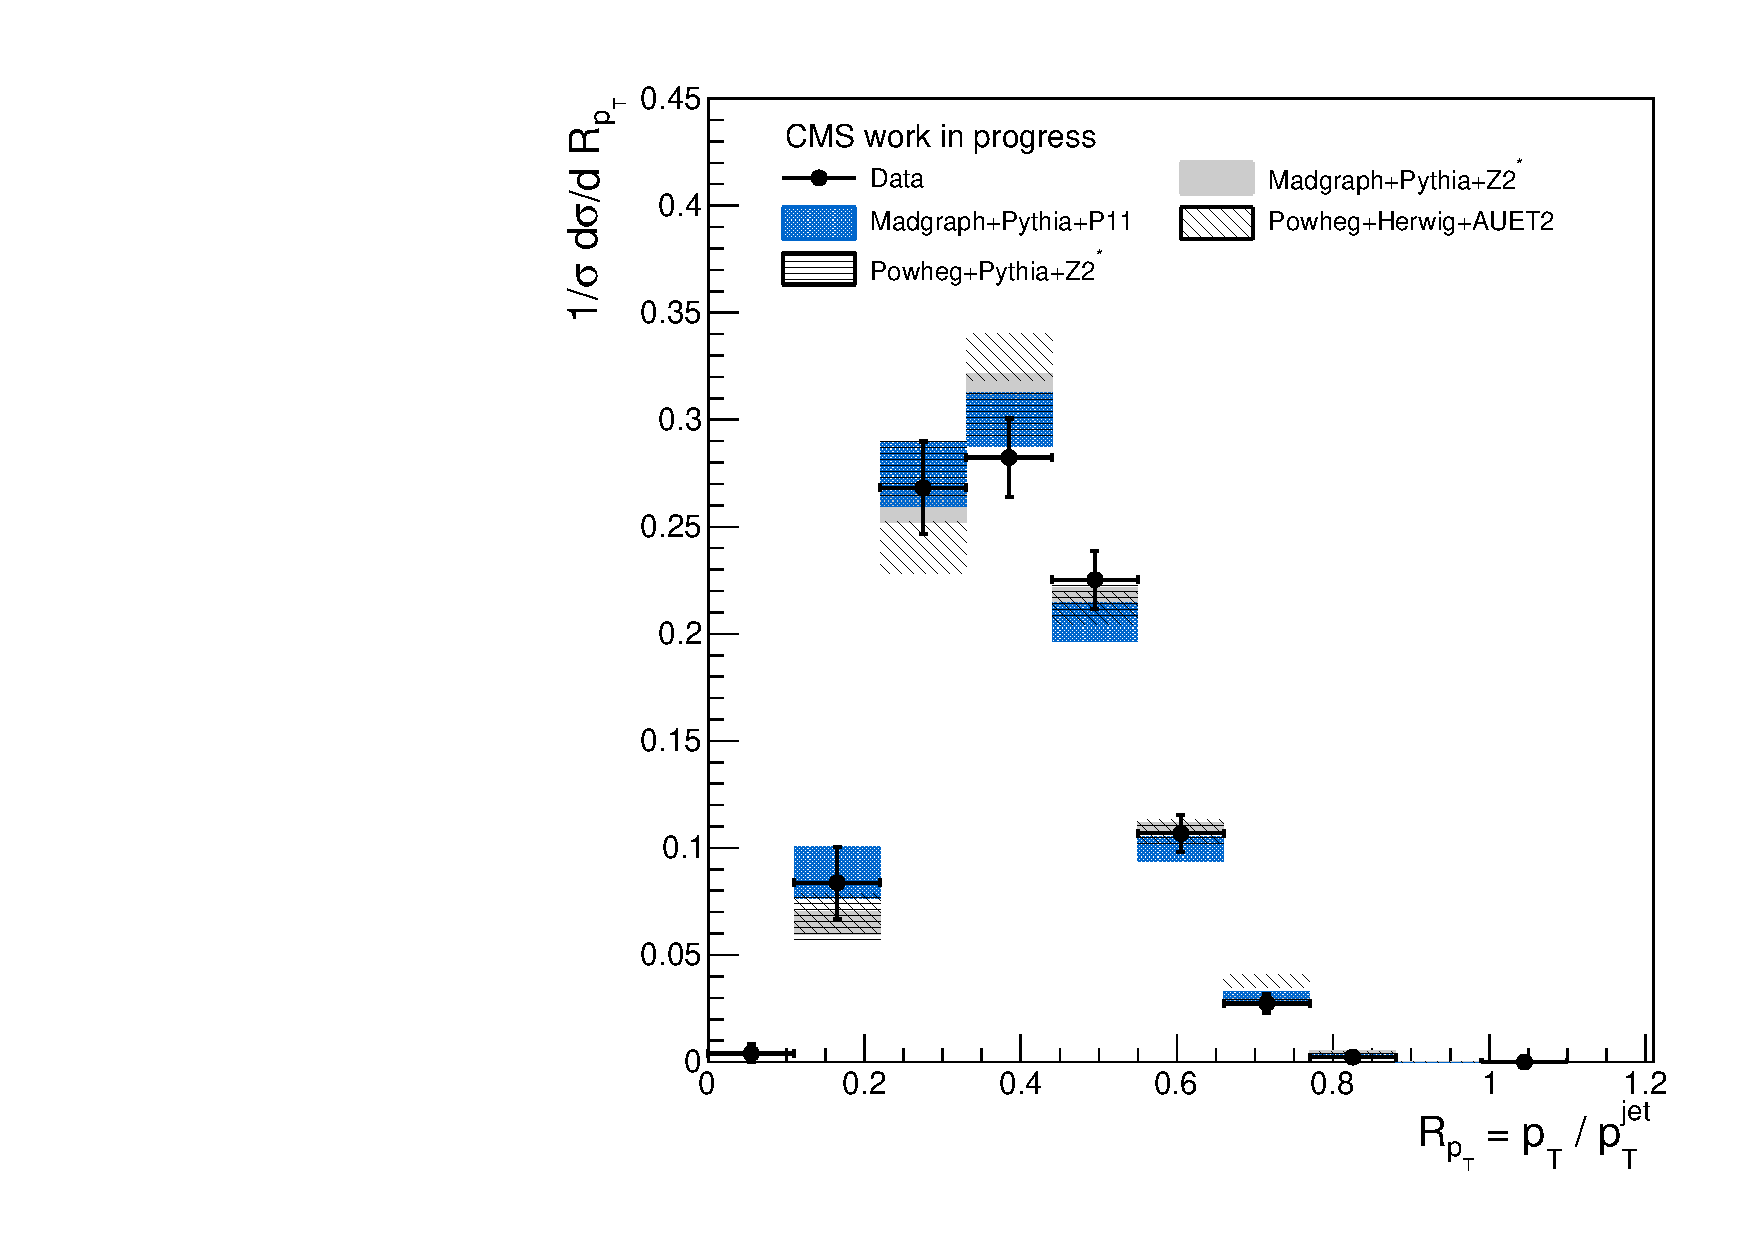
\includegraphics[width=0.32\textwidth]{img/charm/D0Incl3Trk_ptfrac}}
\subfloat[][]{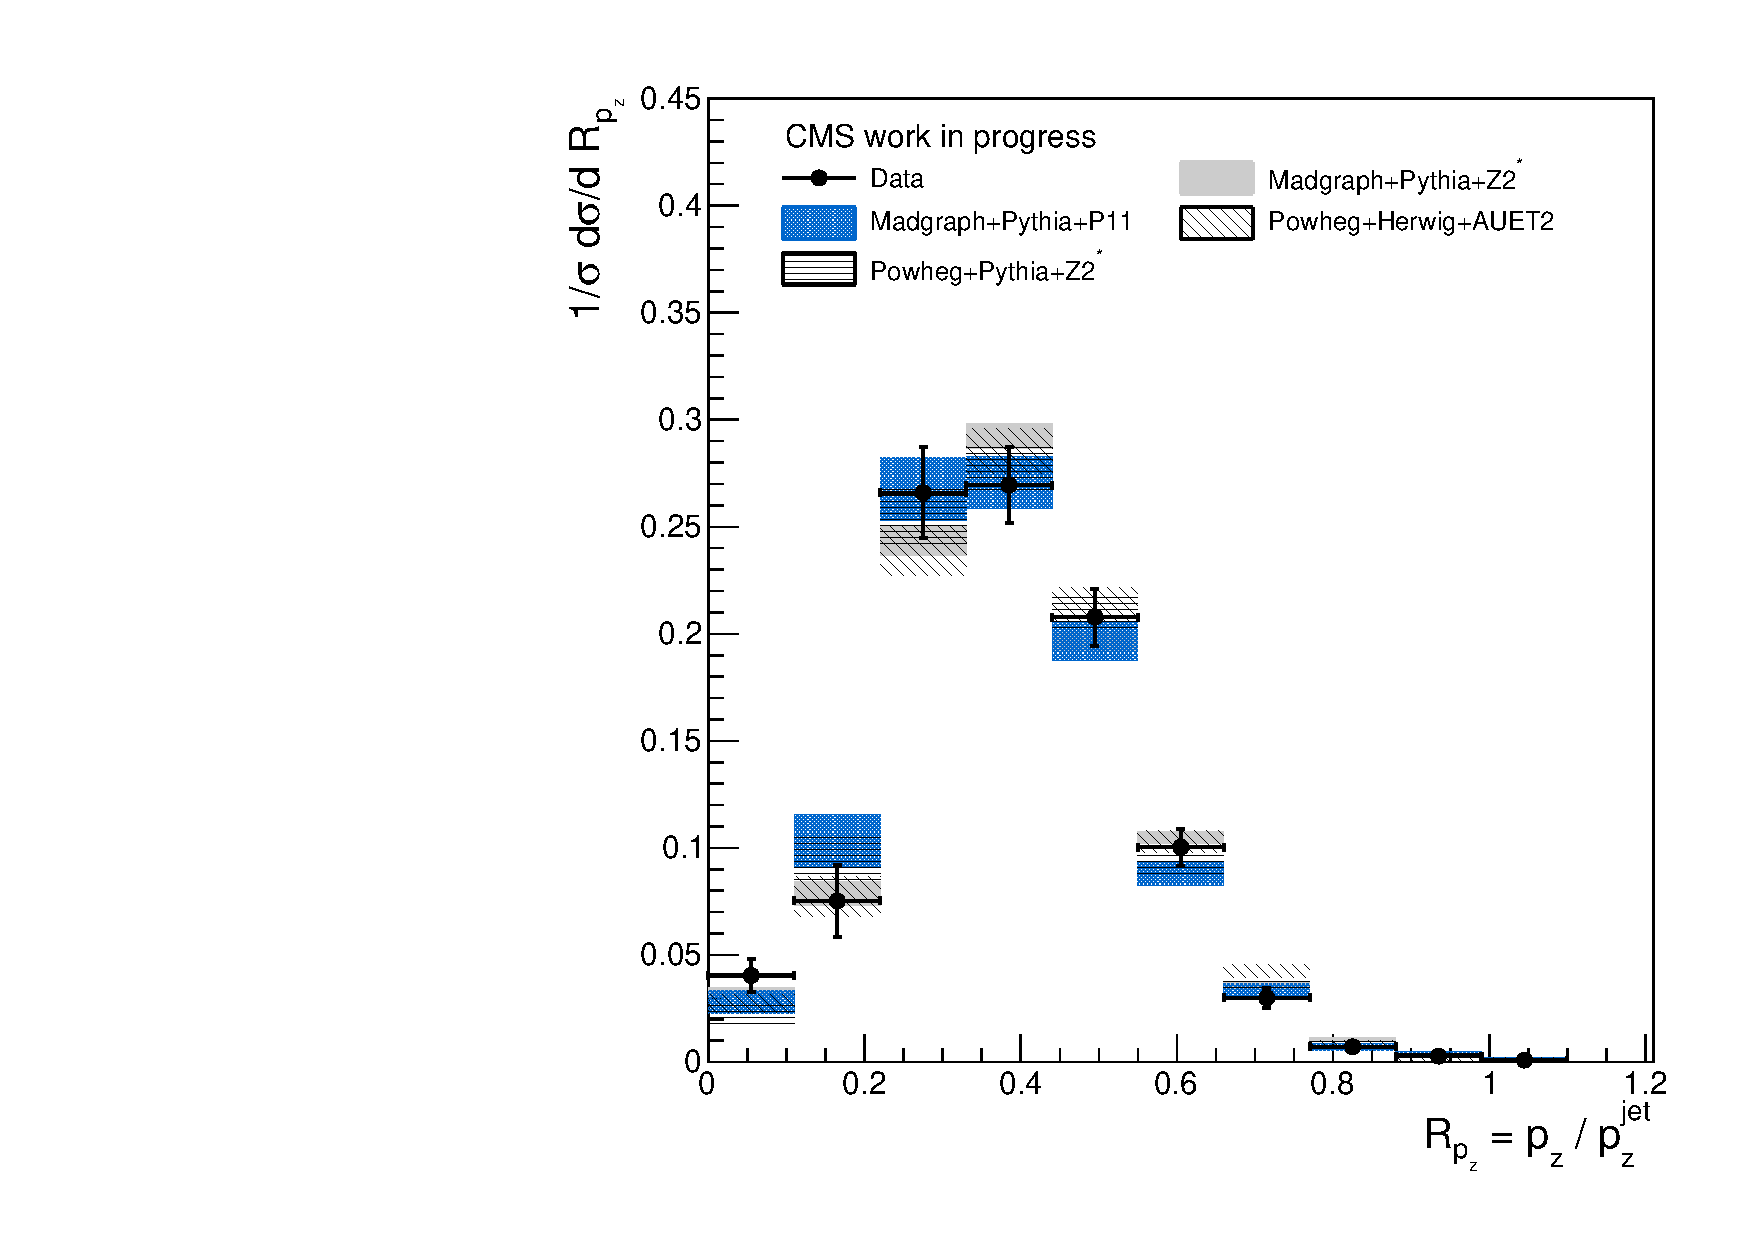
\includegraphics[width=0.32\textwidth]{img/charm/D0Incl3Trk_pzfrac}}\\
\subfloat[][]{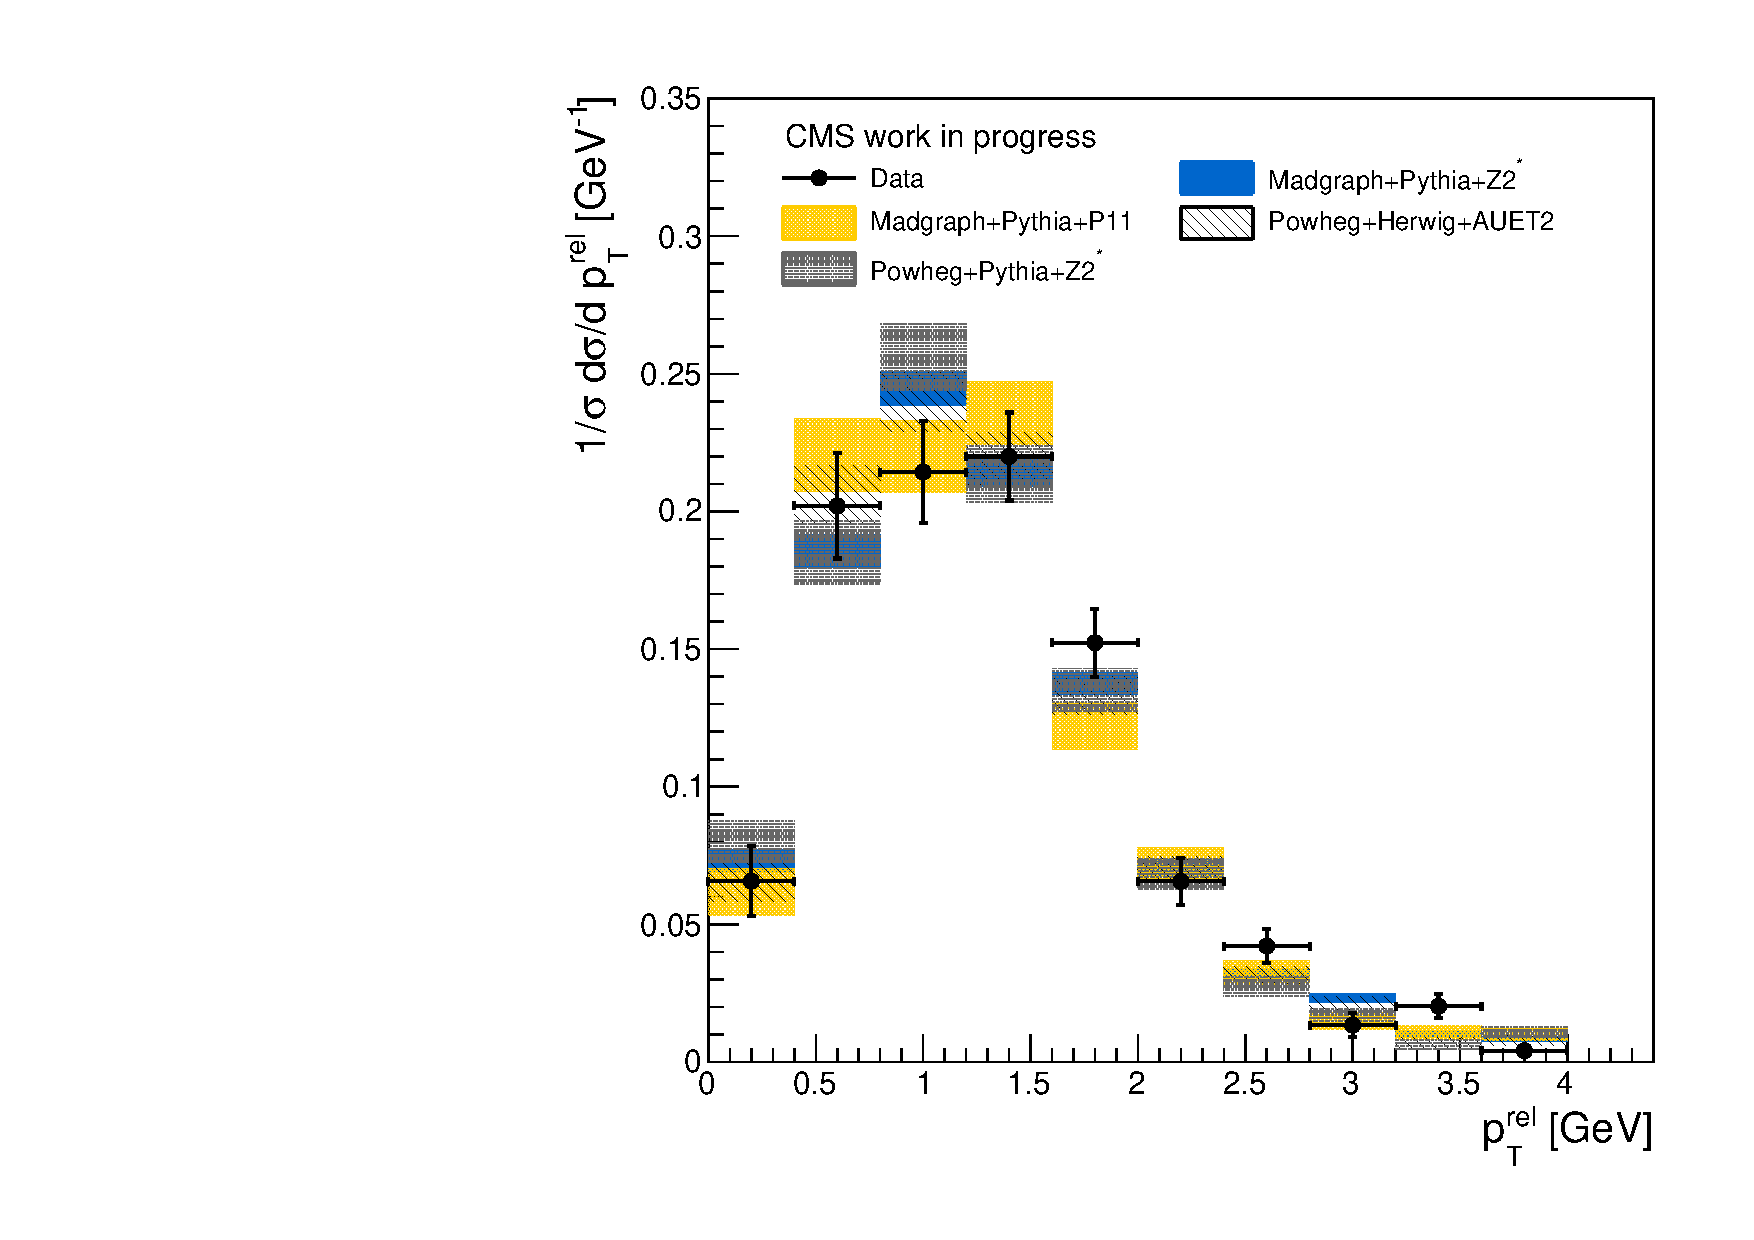
\includegraphics[width=0.32\textwidth]{img/charm/D0Incl3Trk_ptrel}}
\subfloat[][]{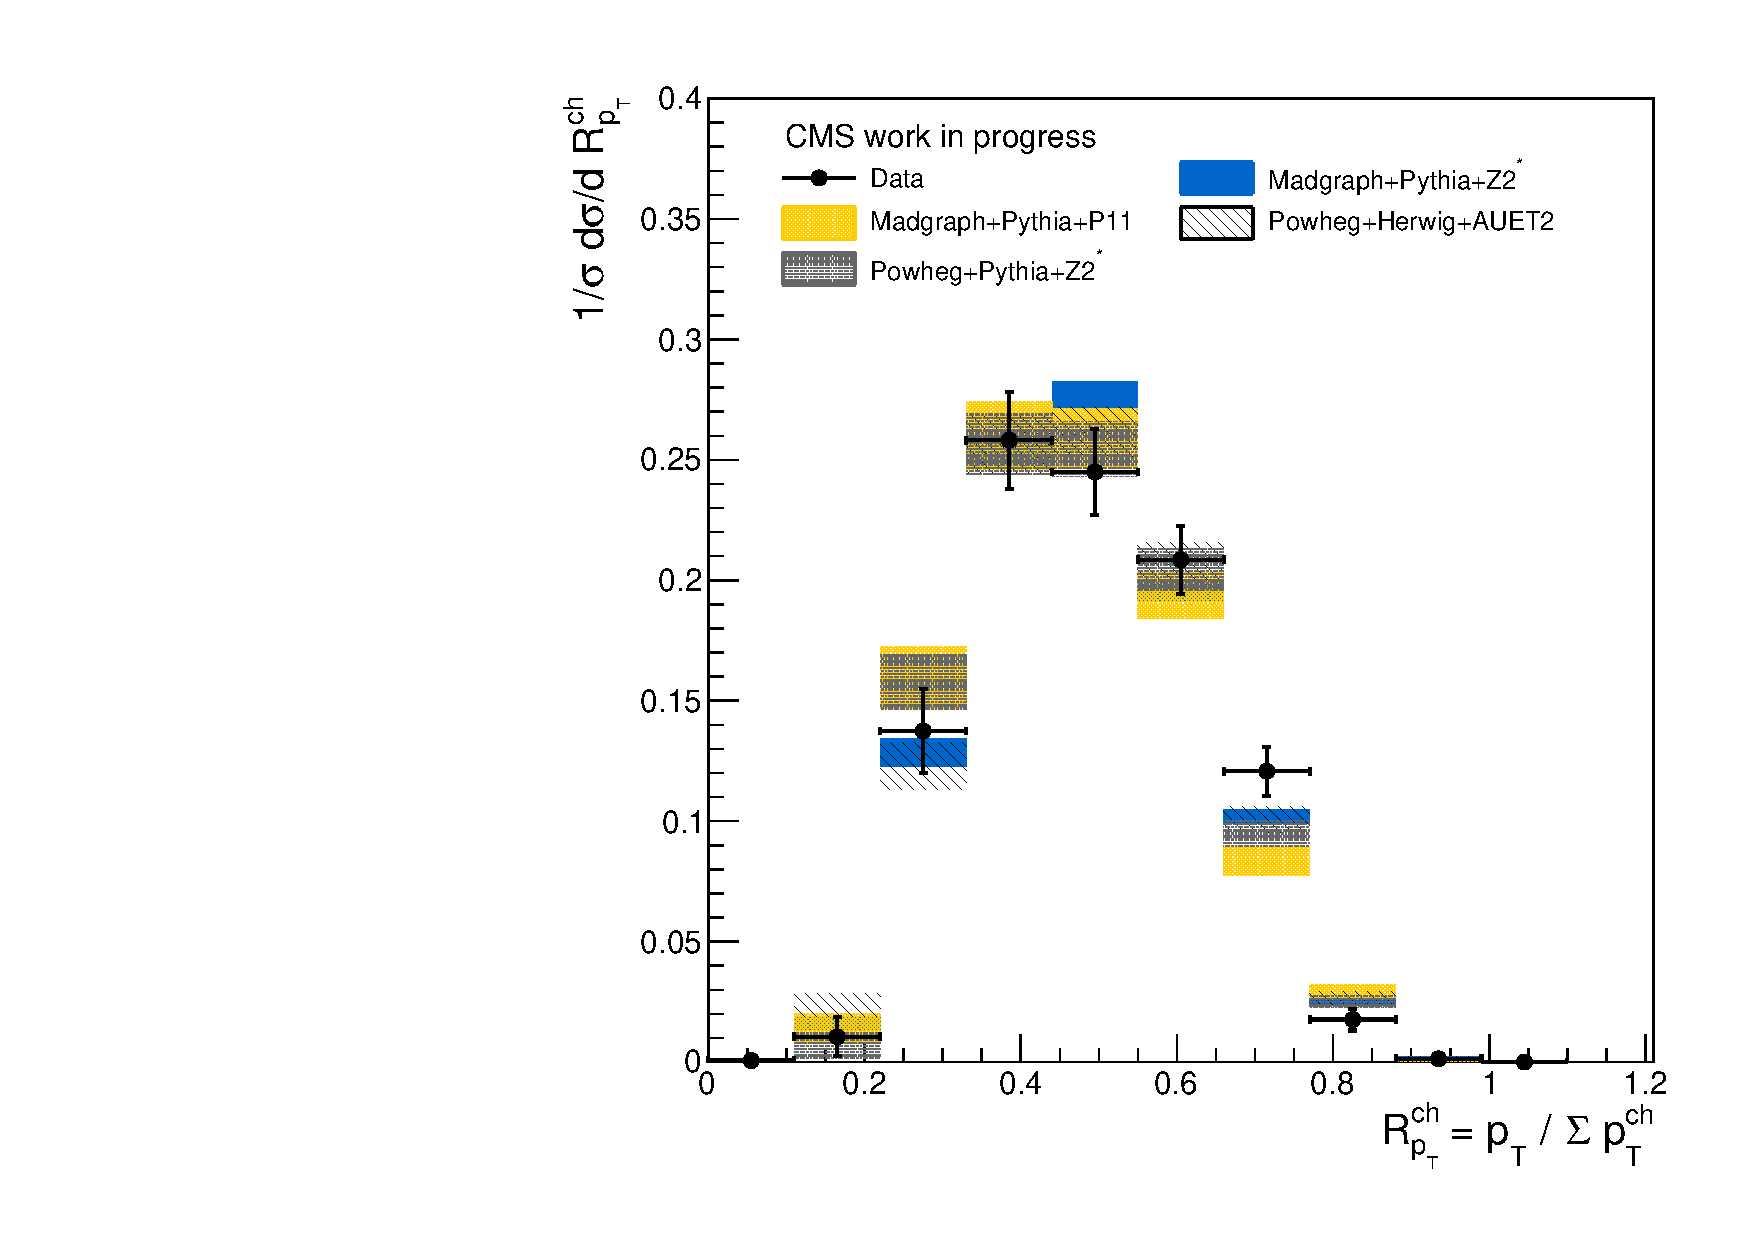
\includegraphics[width=0.32\textwidth]{img/charm/D0Incl3Trk_ptchfrac}}
\subfloat[][]{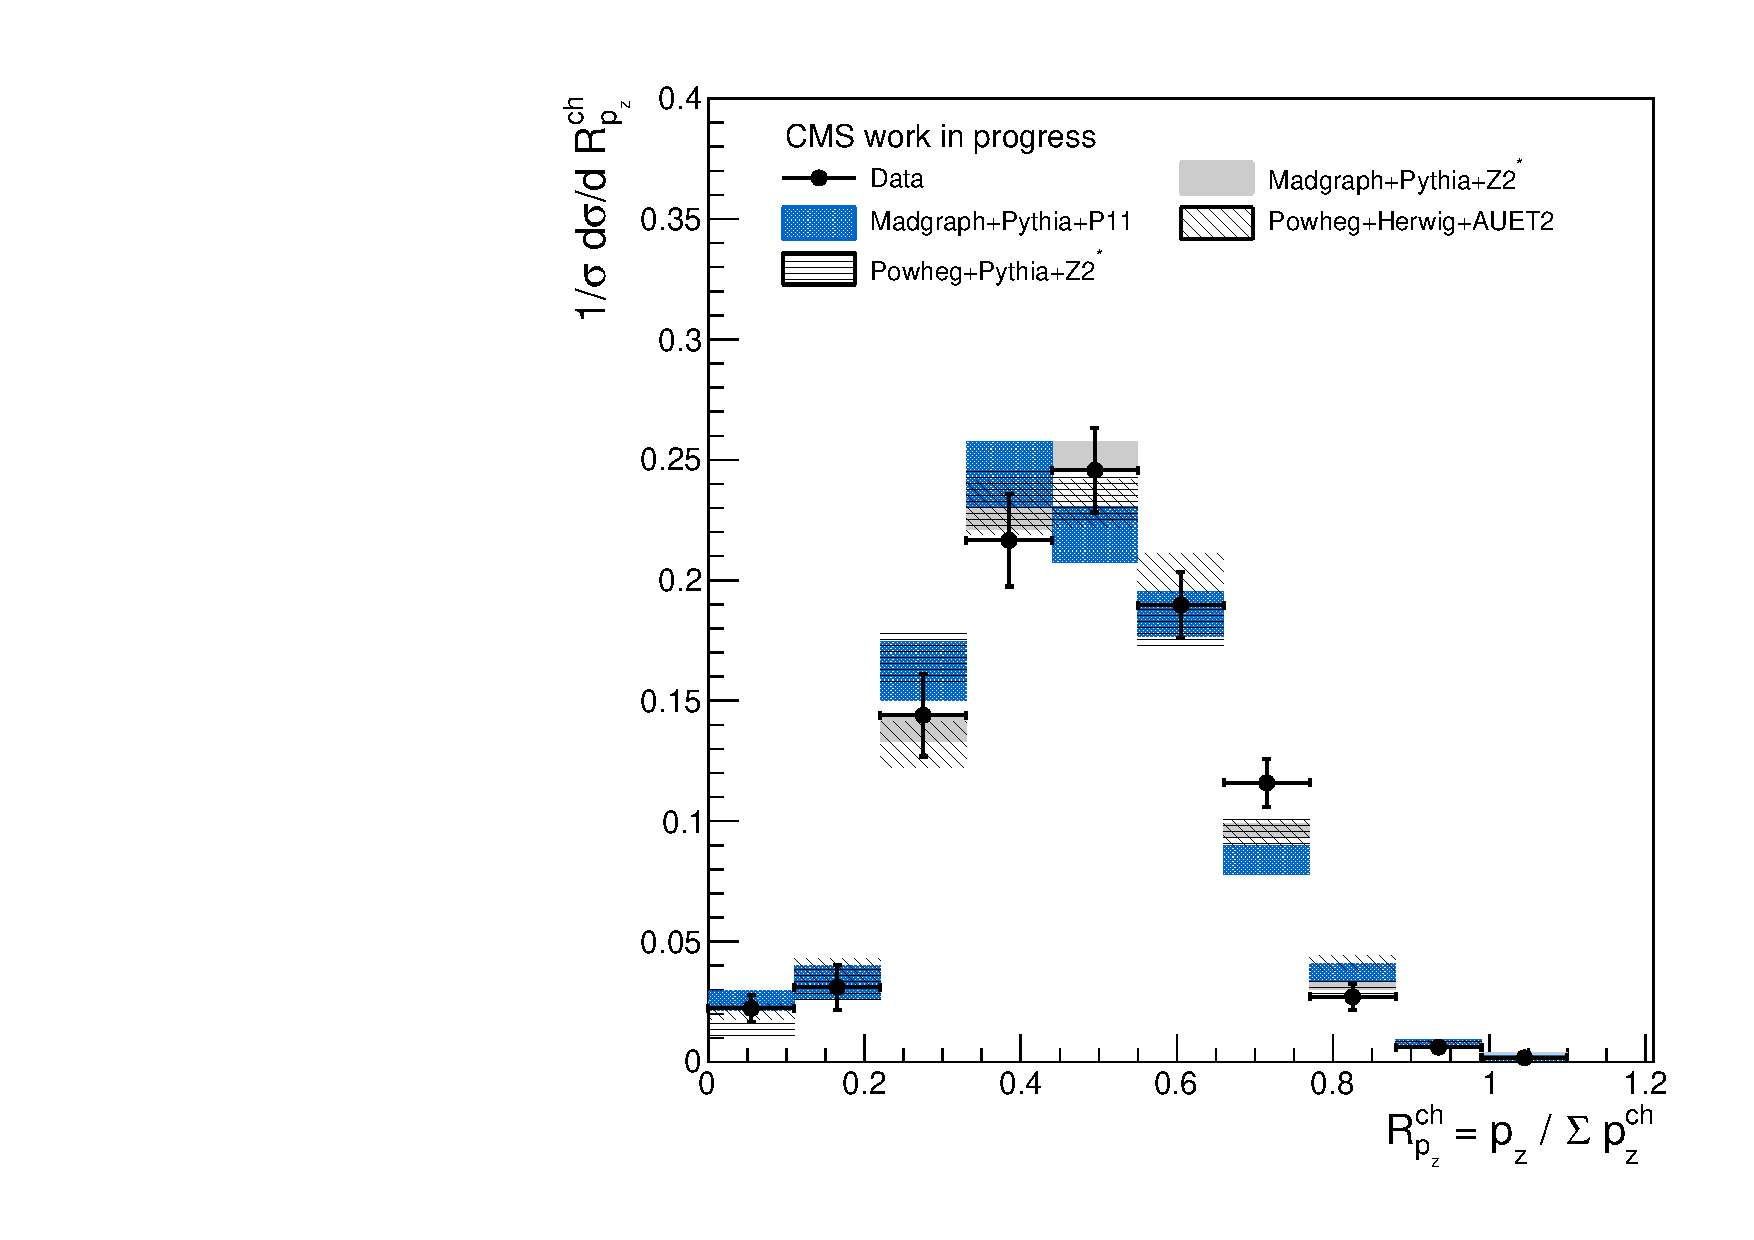
\includegraphics[width=0.32\textwidth]{img/charm/D0Incl3Trk_pzchfrac}}\\
\subfloat[][]{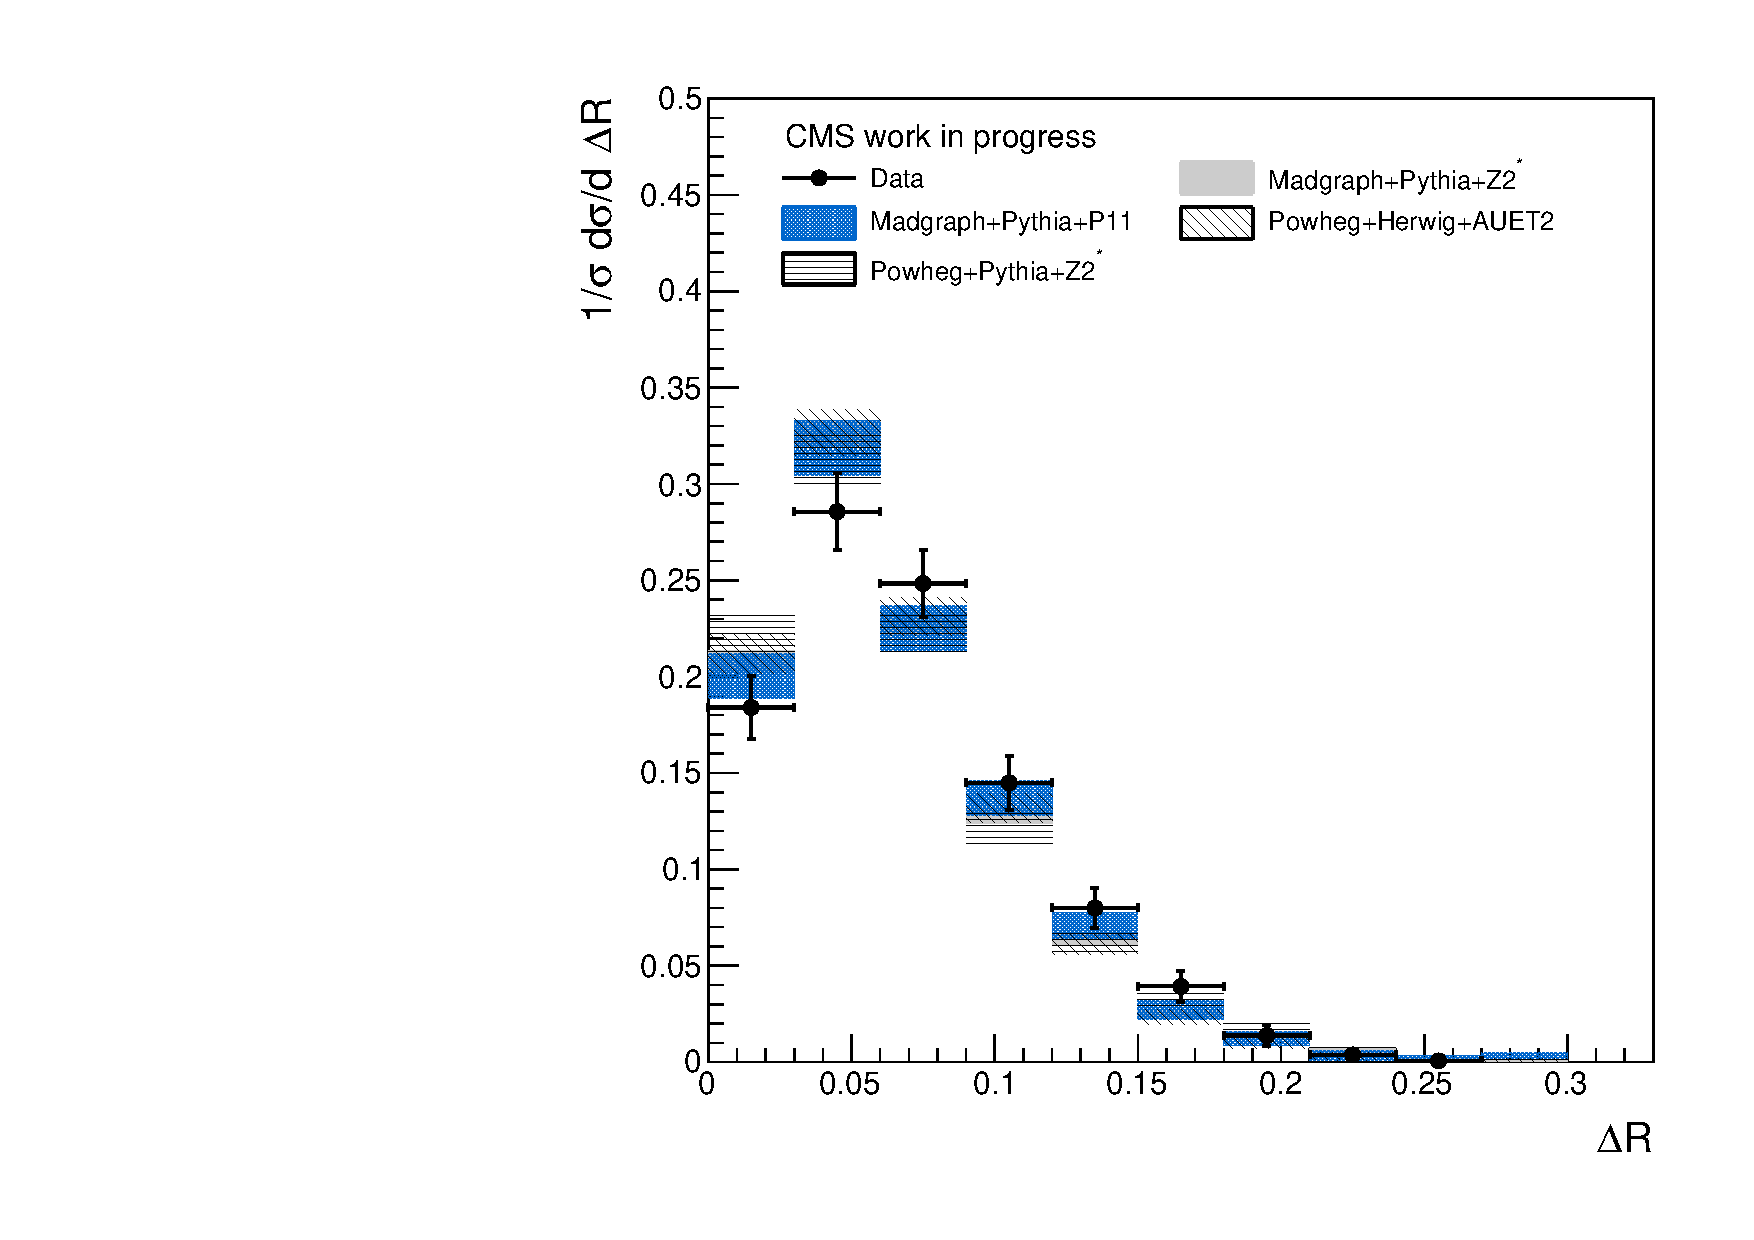
\includegraphics[width=0.32\textwidth]{img/charm/D0Incl3Trk_deltar}}
\caption{ 
Normalized differential production cross sections of $D^0$ meson candidates in \ttbar events, as function of:
(a) $R_p$, (b) $R_{p_{\rm T}}$,  (c) $R_{p_{\rm z}}$, (d) \ptrel, 
(e) $R^{\rm ch}_{p_{\rm T}}$, (f) $R^{\rm ch}_{p_{\rm z}}$ and (e) $\Delta R$.
The expectations for different \ttbar models are shown as shaded bands while the data is shown as marker points.
Bin-center corrections have been applied to both data and MC.
}
\label{fig:d0kinematics}
\end{figure}

\begin{figure}[htp] 
\centering
\subfloat[][]{\includegraphics[width=0.32\textwidth]{img/charm/D0lep_pfrac}}
\subfloat[][]{\includegraphics[width=0.32\textwidth]{img/charm/D0lep_ptfrac}}
\subfloat[][]{\includegraphics[width=0.32\textwidth]{img/charm/D0lep_pzfrac}}\\
\subfloat[][]{\includegraphics[width=0.32\textwidth]{img/charm/D0lep_ptrel}}
\subfloat[][]{\includegraphics[width=0.32\textwidth]{img/charm/D0lep_ptchfrac}}
\subfloat[][]{\includegraphics[width=0.32\textwidth]{img/charm/D0lep_pzchfrac}}\\
\subfloat[][]{\includegraphics[width=0.32\textwidth]{img/charm/D0lep_deltar}}
\caption{ 
Similar to Fig.~\ref{fig:d0kinematics} for $D^0$ meson candidates reconstructed with a soft lepton tag.
}
\label{fig:d0lepkinematics}
\end{figure}

\begin{figure}[htp] 
\centering
\subfloat[][]{\includegraphics[width=0.32\textwidth]{img/charm/DpmZ0_pfrac}}
\subfloat[][]{\includegraphics[width=0.32\textwidth]{img/charm/DpmZ0_ptfrac}}
\subfloat[][]{\includegraphics[width=0.32\textwidth]{img/charm/DpmZ0_pzfrac}}\\
\subfloat[][]{\includegraphics[width=0.32\textwidth]{img/charm/DpmZ0_ptrel}}
\subfloat[][]{\includegraphics[width=0.32\textwidth]{img/charm/DpmZ0_ptchfrac}}
\subfloat[][]{\includegraphics[width=0.32\textwidth]{img/charm/DpmZ0_pzchfrac}}\\
\subfloat[][]{\includegraphics[width=0.32\textwidth]{img/charm/DpmZ0_deltar}}
\caption{ 
Similar to Fig.~\ref{fig:d0kinematics} for $D^\pm$.
}
\label{fig:dpmkinematics}
\end{figure}

\begin{figure}[htp] 
\centering
\subfloat[][]{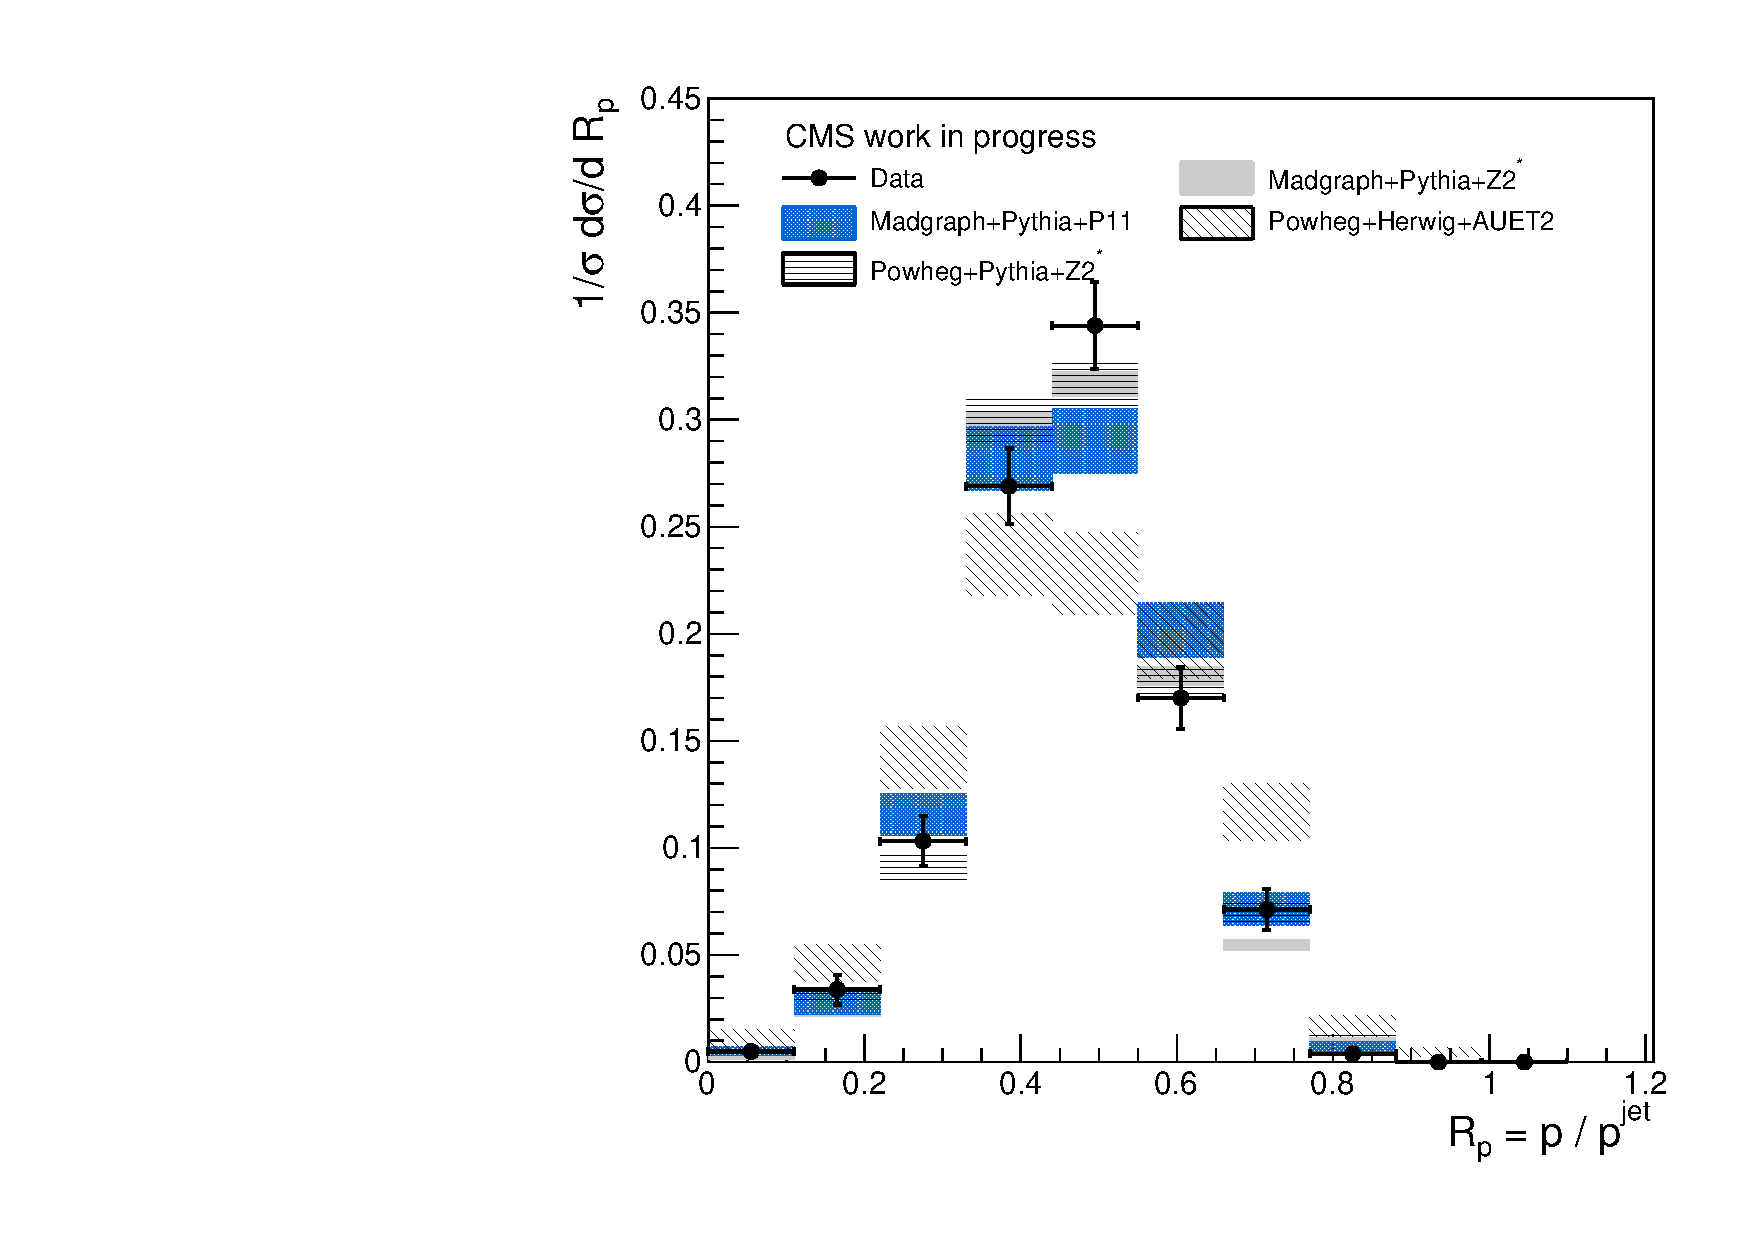
\includegraphics[width=0.32\textwidth]{img/charm/JPsi_pfrac}}
\subfloat[][]{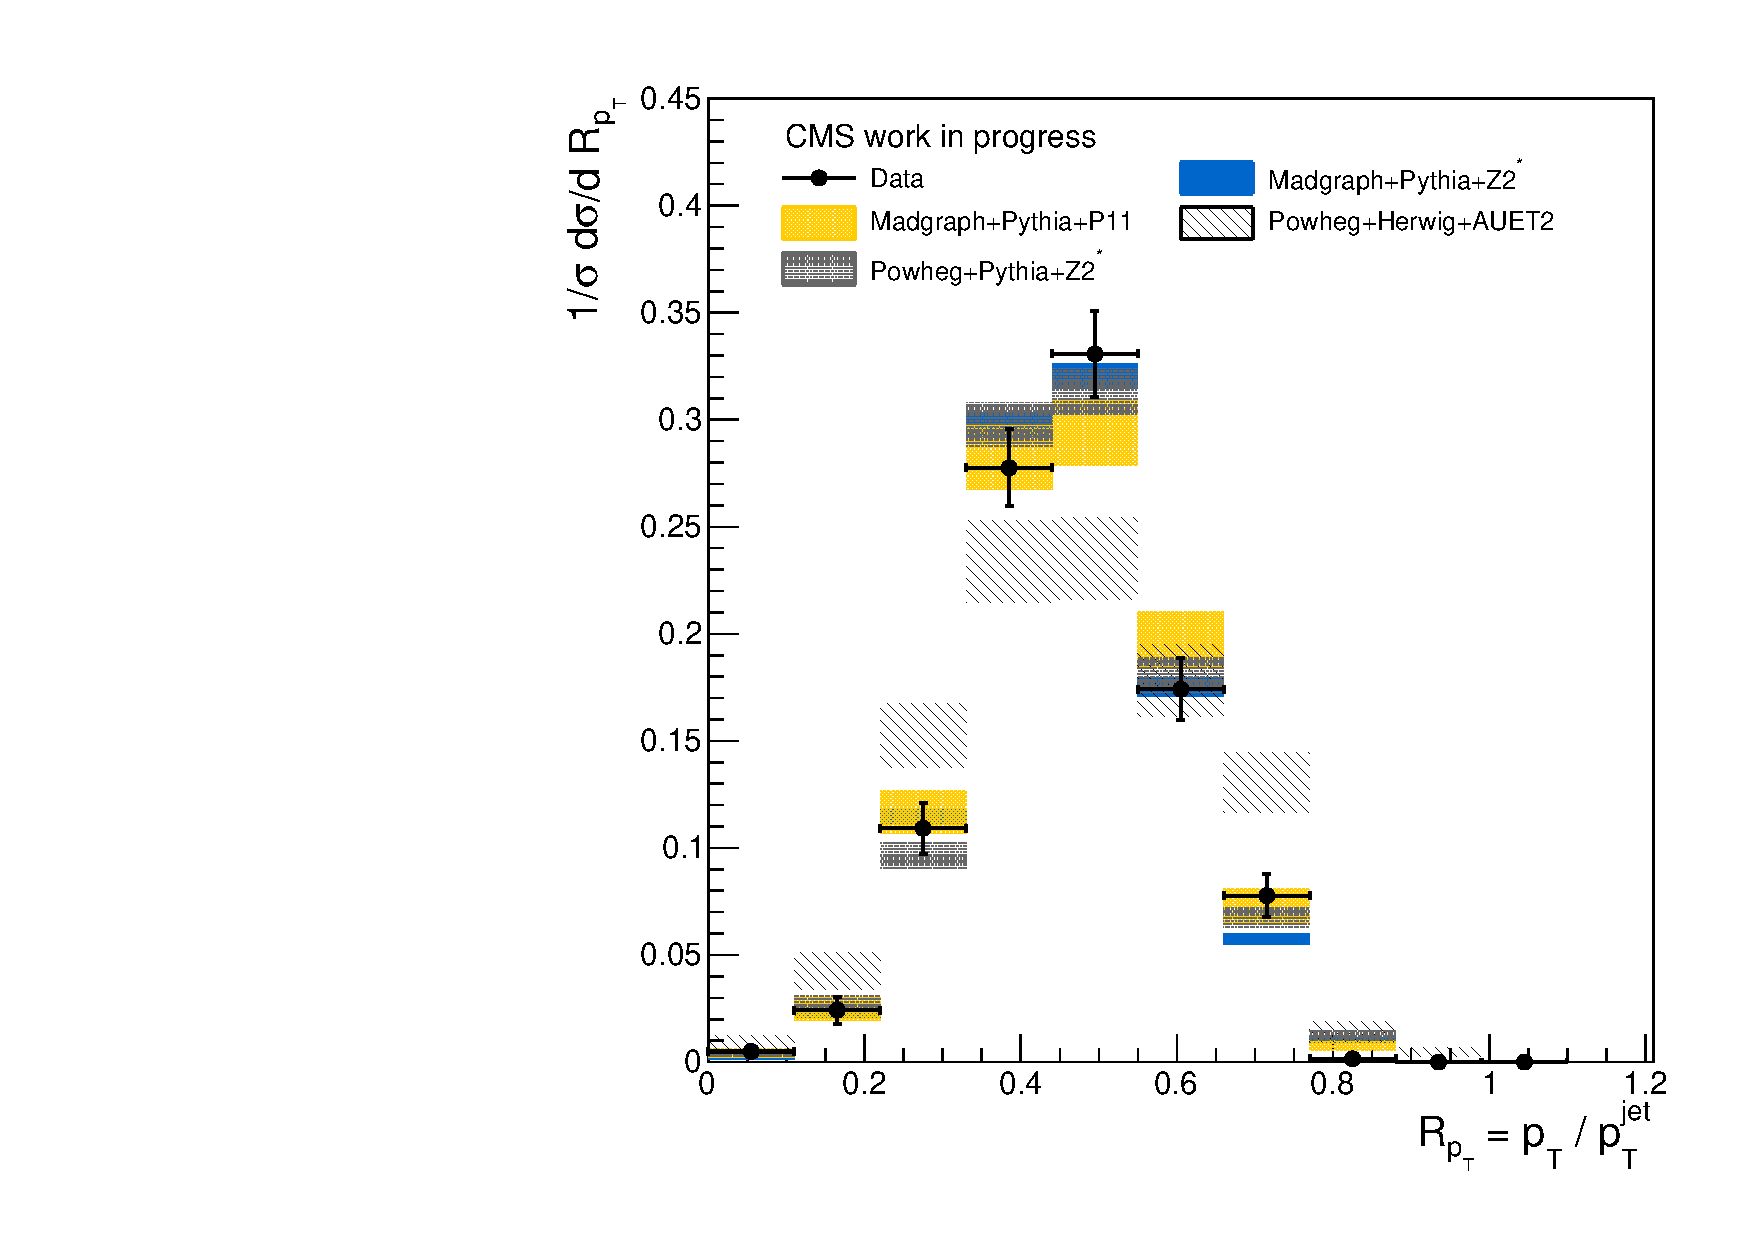
\includegraphics[width=0.32\textwidth]{img/charm/JPsi_ptfrac}}
\subfloat[][]{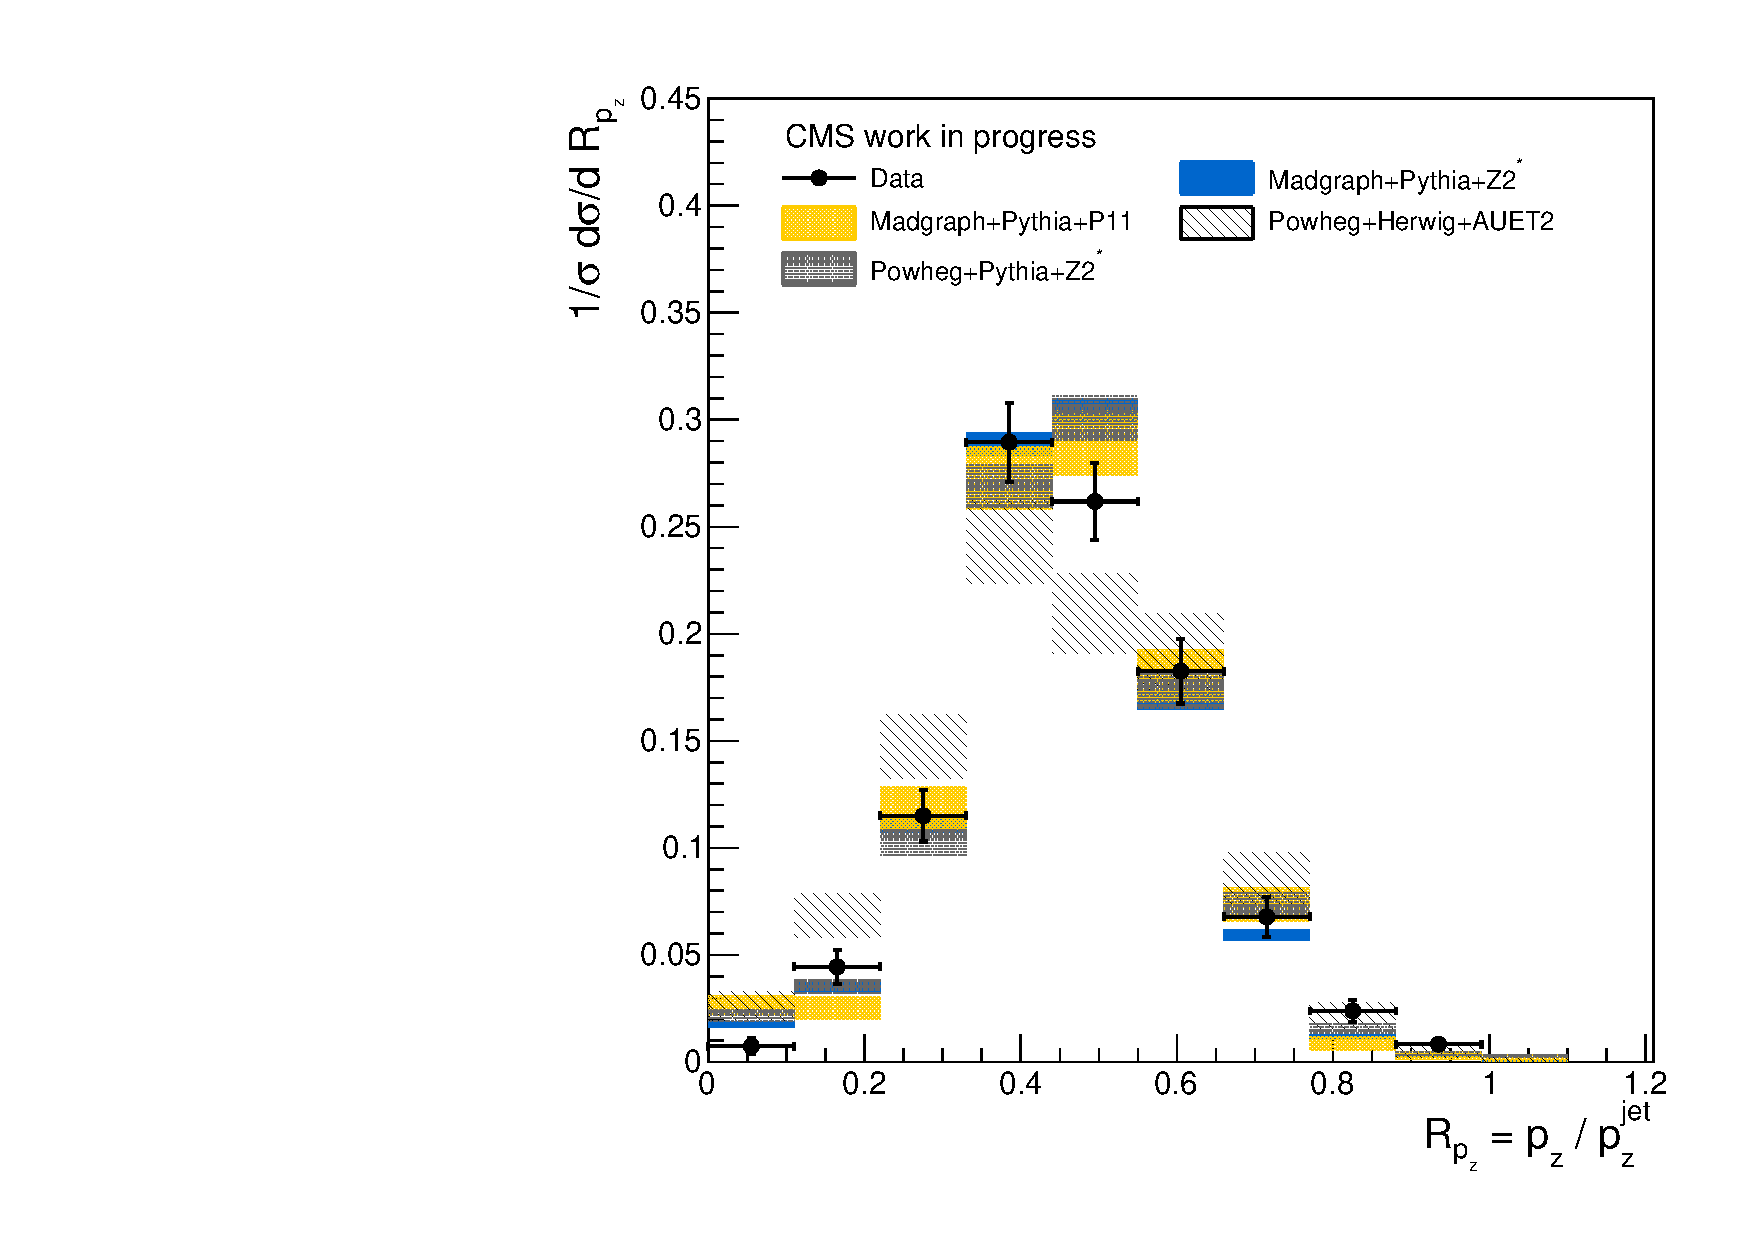
\includegraphics[width=0.32\textwidth]{img/charm/JPsi_pzfrac}}\\
\subfloat[][]{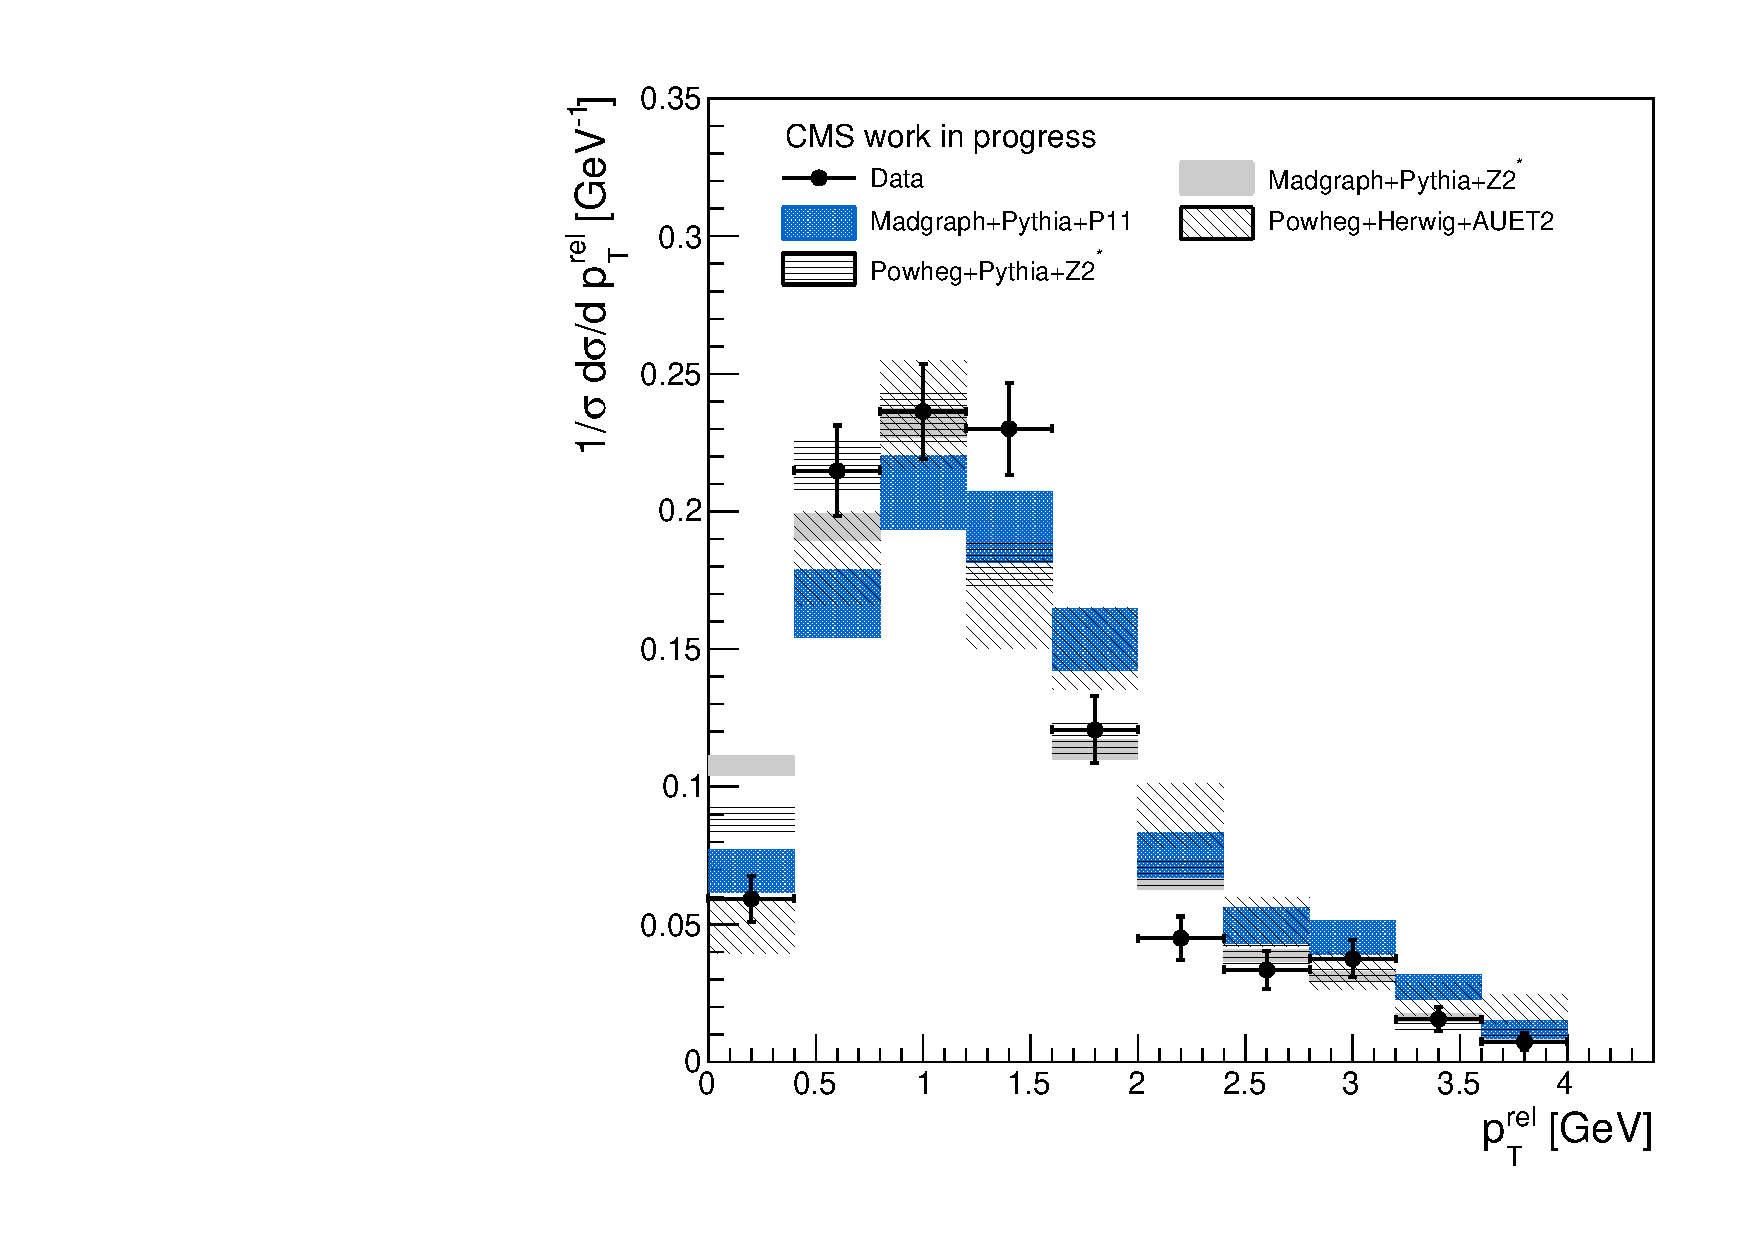
\includegraphics[width=0.32\textwidth]{img/charm/JPsi_ptrel}}
\subfloat[][]{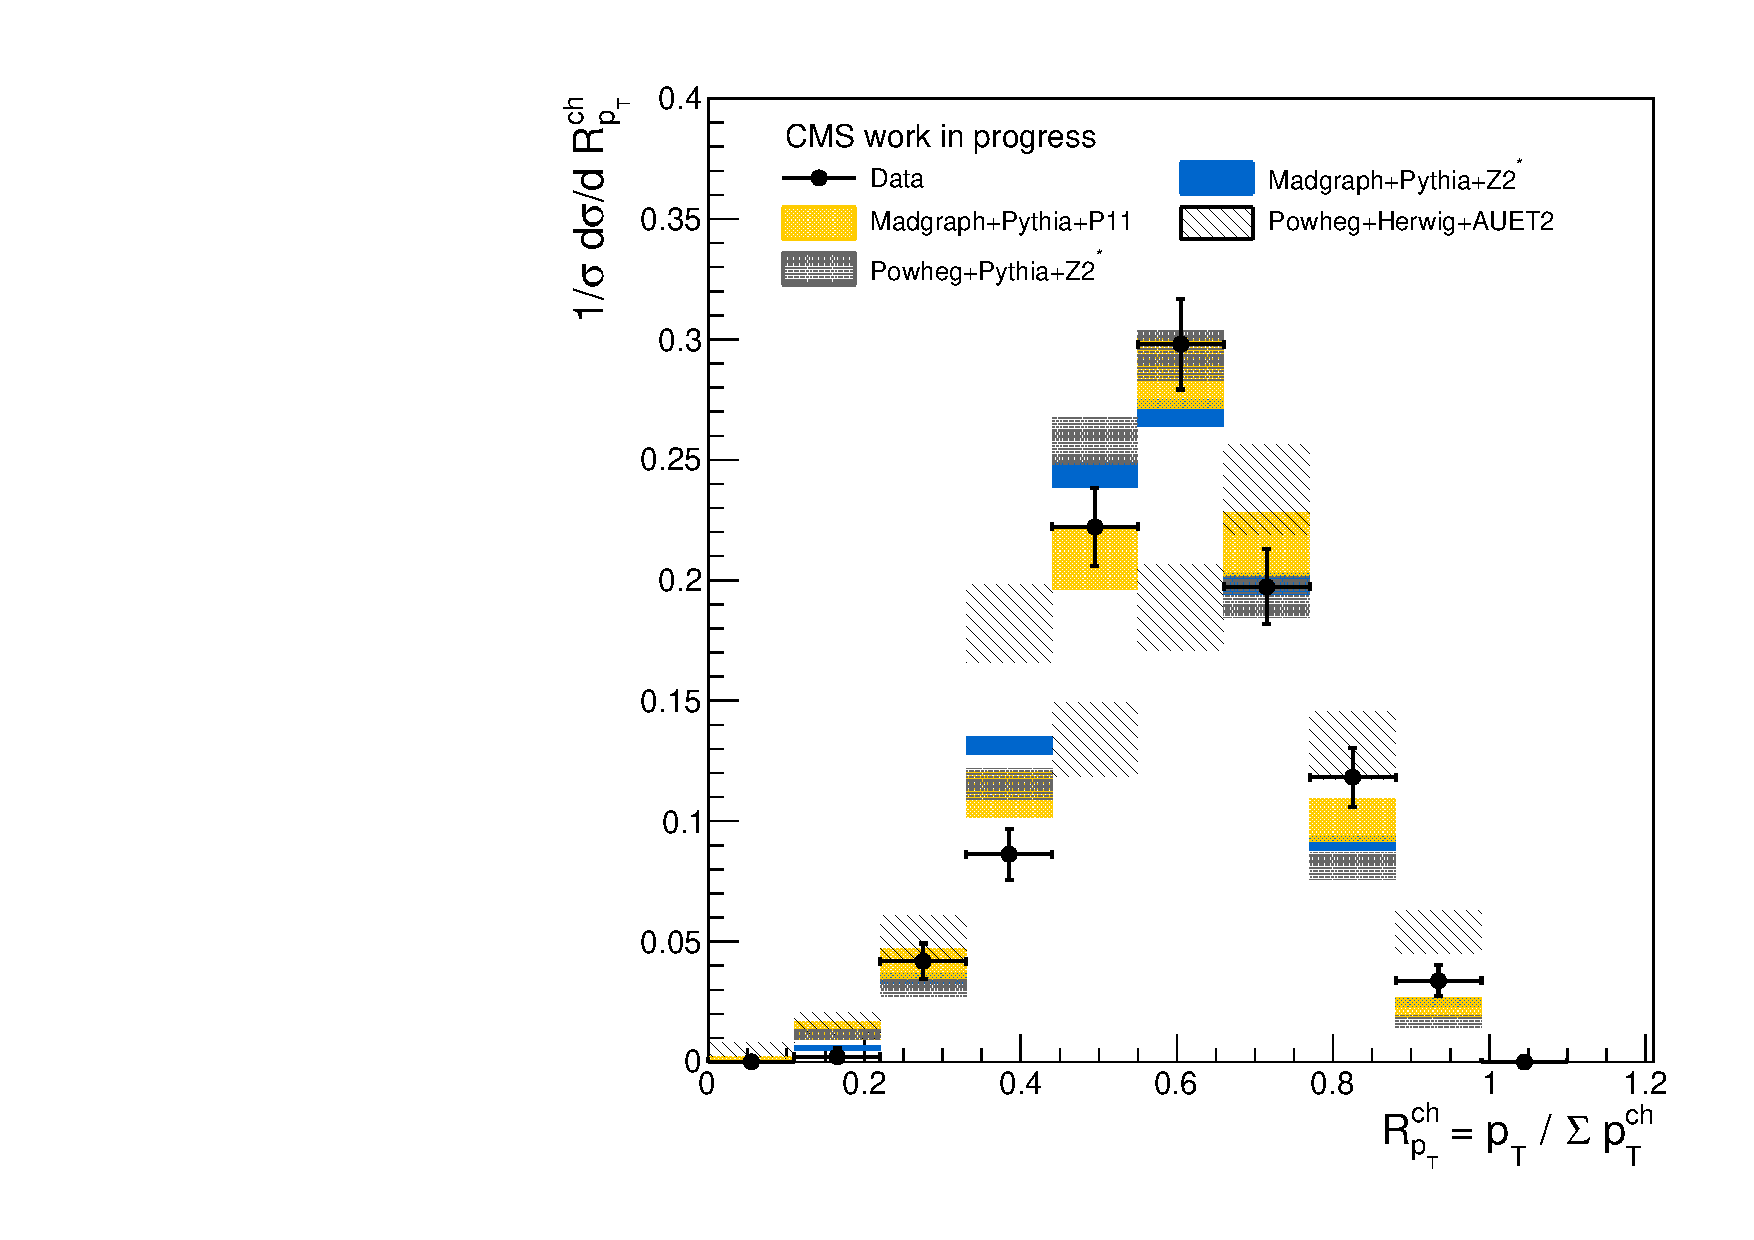
\includegraphics[width=0.32\textwidth]{img/charm/JPsi_ptchfrac}}
\subfloat[][]{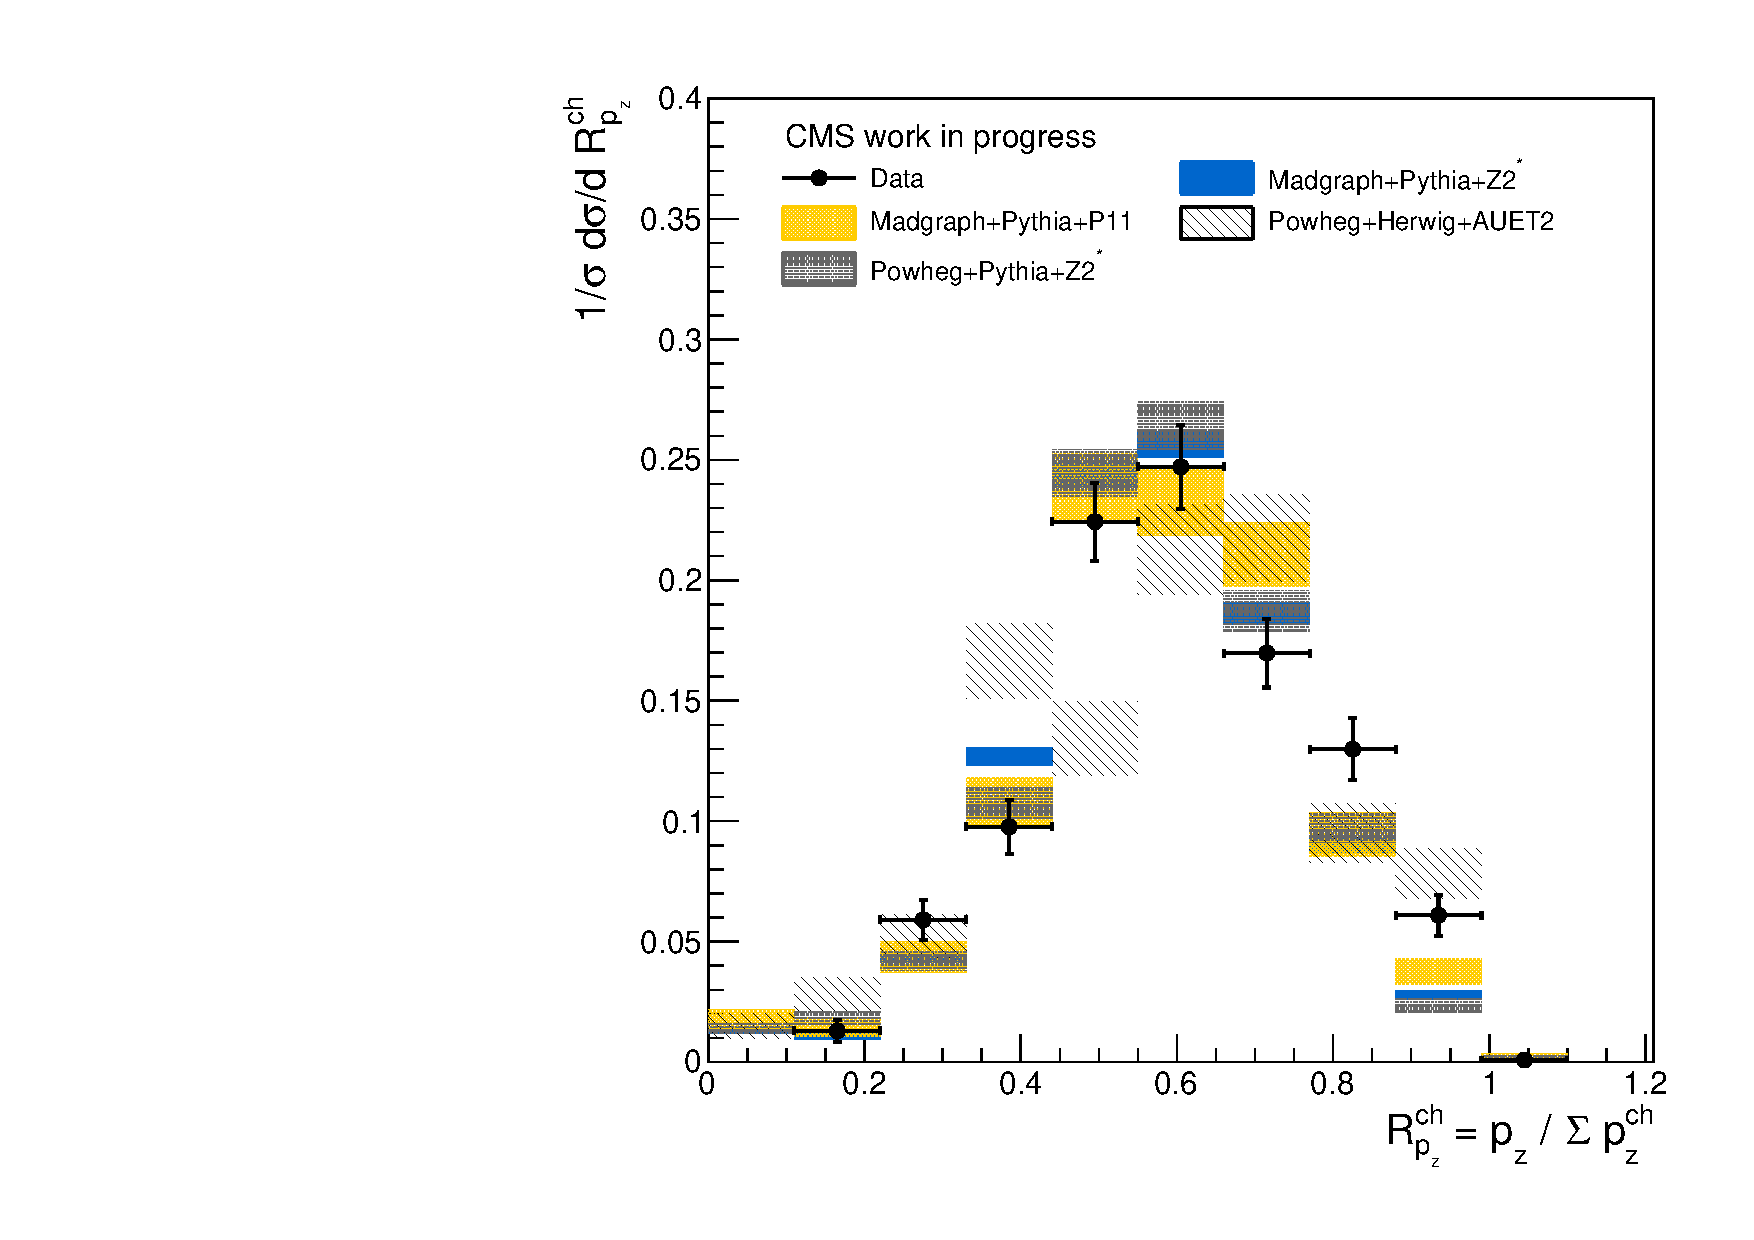
\includegraphics[width=0.32\textwidth]{img/charm/JPsi_pzchfrac}}\\
\subfloat[][]{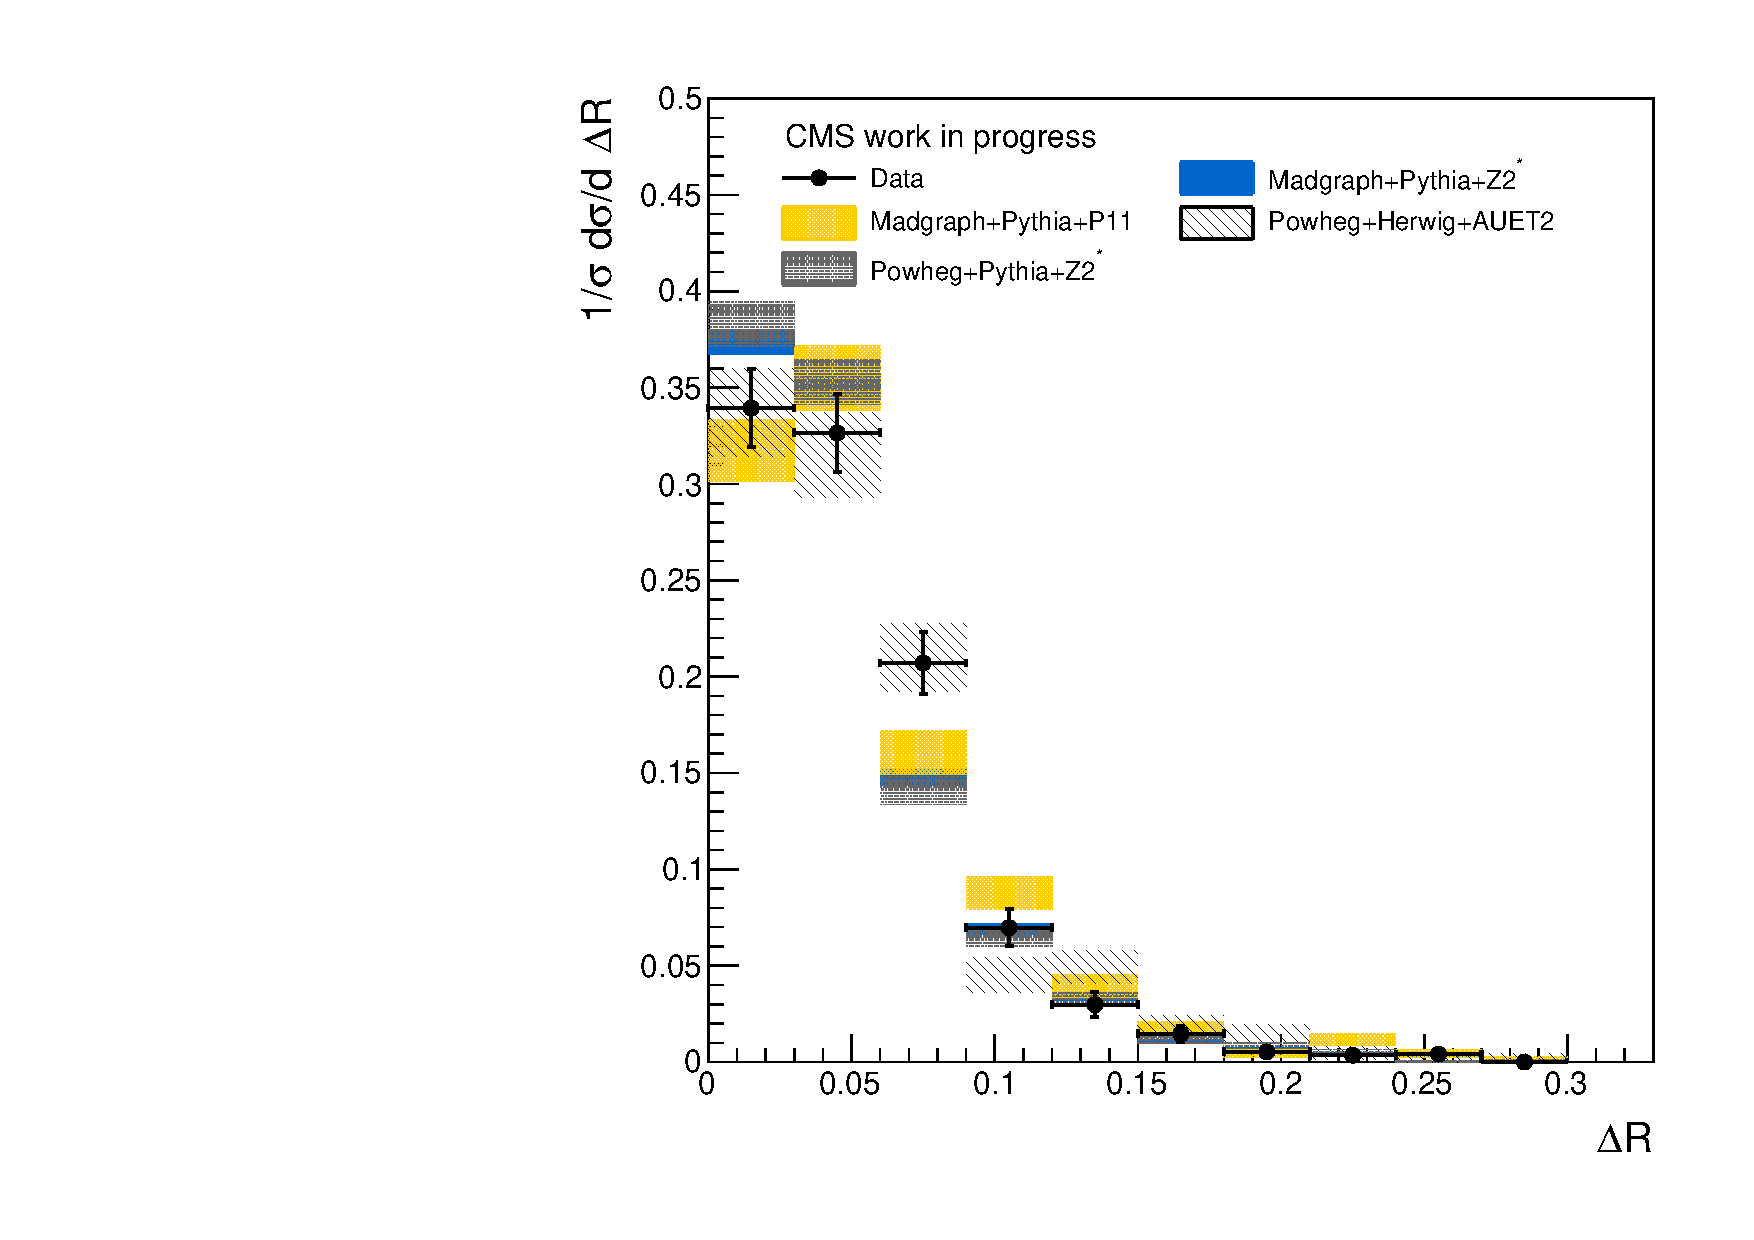
\includegraphics[width=0.32\textwidth]{img/charm/JPsi_deltar}}
\caption{ 
Similar to Fig.~\ref{fig:d0kinematics} for $J/\psi$.
}
\label{fig:jpsikinematics}
\end{figure}

%%
%%
%%
\clearpage
\section{Secondary vertex reconstruction: performance in a control dijet sample}
\label{sec:secvertexqcd}

In order to test the performance of the algorithm used to reconstruct secondary vertices
we use a control sample which is orthogonal to the one used in our measurement.
Dijet events, where the tagging object is a jet with $\pt>30\GeV$ which is required to contain
a muon and to pass the CSV loose working point are selected in data and compared to the 
expections from simulation. Dedicated $b$-tag triggers are used to collect this sample,
as described in Sec.~\ref{sec:datasetsandselection}.

For each event we probe the second jet in the event
if it contains a reconstructed secondary vertex 
and if $\Delta\phi(j_1,j_2)>2.7$ and $0.7<p_{\rm T}^1/p_{\rm T}^2<1.3$
(recoil condition).
The distribution of the secondary vertex mass (SecVtx mass) of the probe jet is used to estimate its flavor composition.
The secondary vertex mass has distinctive characteristics for $\cPqb$, $\cPqc$ and udsg jets
which can be used to fit to the distribution observed in data.
For this purposed we use the probability distribution functions of the SecVtx mass as predicted in simulation.
An extended, binned, likelihood is then maximized in order do estimate the flavor composition.
In the fit we float freely the number light flavoured jets (\ie udsg) and the total number of heavy-flavoured jets (\ie $\cPqb$+$\cPqc$).
The relative ratio between $\cPqb$- and $\cPqc$-jets is assumed from simulation.
We have also tested that relaxing this assumption does not yield significantly different results.
The heavy flavour fit is made in different \pt ranges of the probe jet.

Figure~\ref{fig:svtxmass} shows the distribution of the SecVtx mass.
Besides showing the result in the inclusive sample we split furthermore according to the track multiplcity of the secondary vertex.
The contamination from light jets in the sample for which at least 3 tracks are required is significantly reduced.
Furthermore, if we use the fractions fit to the secondary vertex mass from the inclusive sample
we observe a discrepancy in the description of the track multiplicity 
as summarized in Fig.~\ref{fig:svtx_trkmult} and Fig.~\ref{fig:svtx_trkmult_momenta}.
While the median number of tracks is well reproduced, the same is not true for the width of the distribution,
data yields a steeper distribution than the one predicted by simulation.
This effect is also observed in the \ttbar sample.
In order to understand if this effect can be calibrated away by combining
exclusive \mtop measurements which make use of secondary vertices with different track multiplicities
we explore further the characteristics of the secondary vertices in the exclusive track multiplicity categories.

\begin{landscape}
\begin{figure}[htp] 
\centering
\subfloat[][]{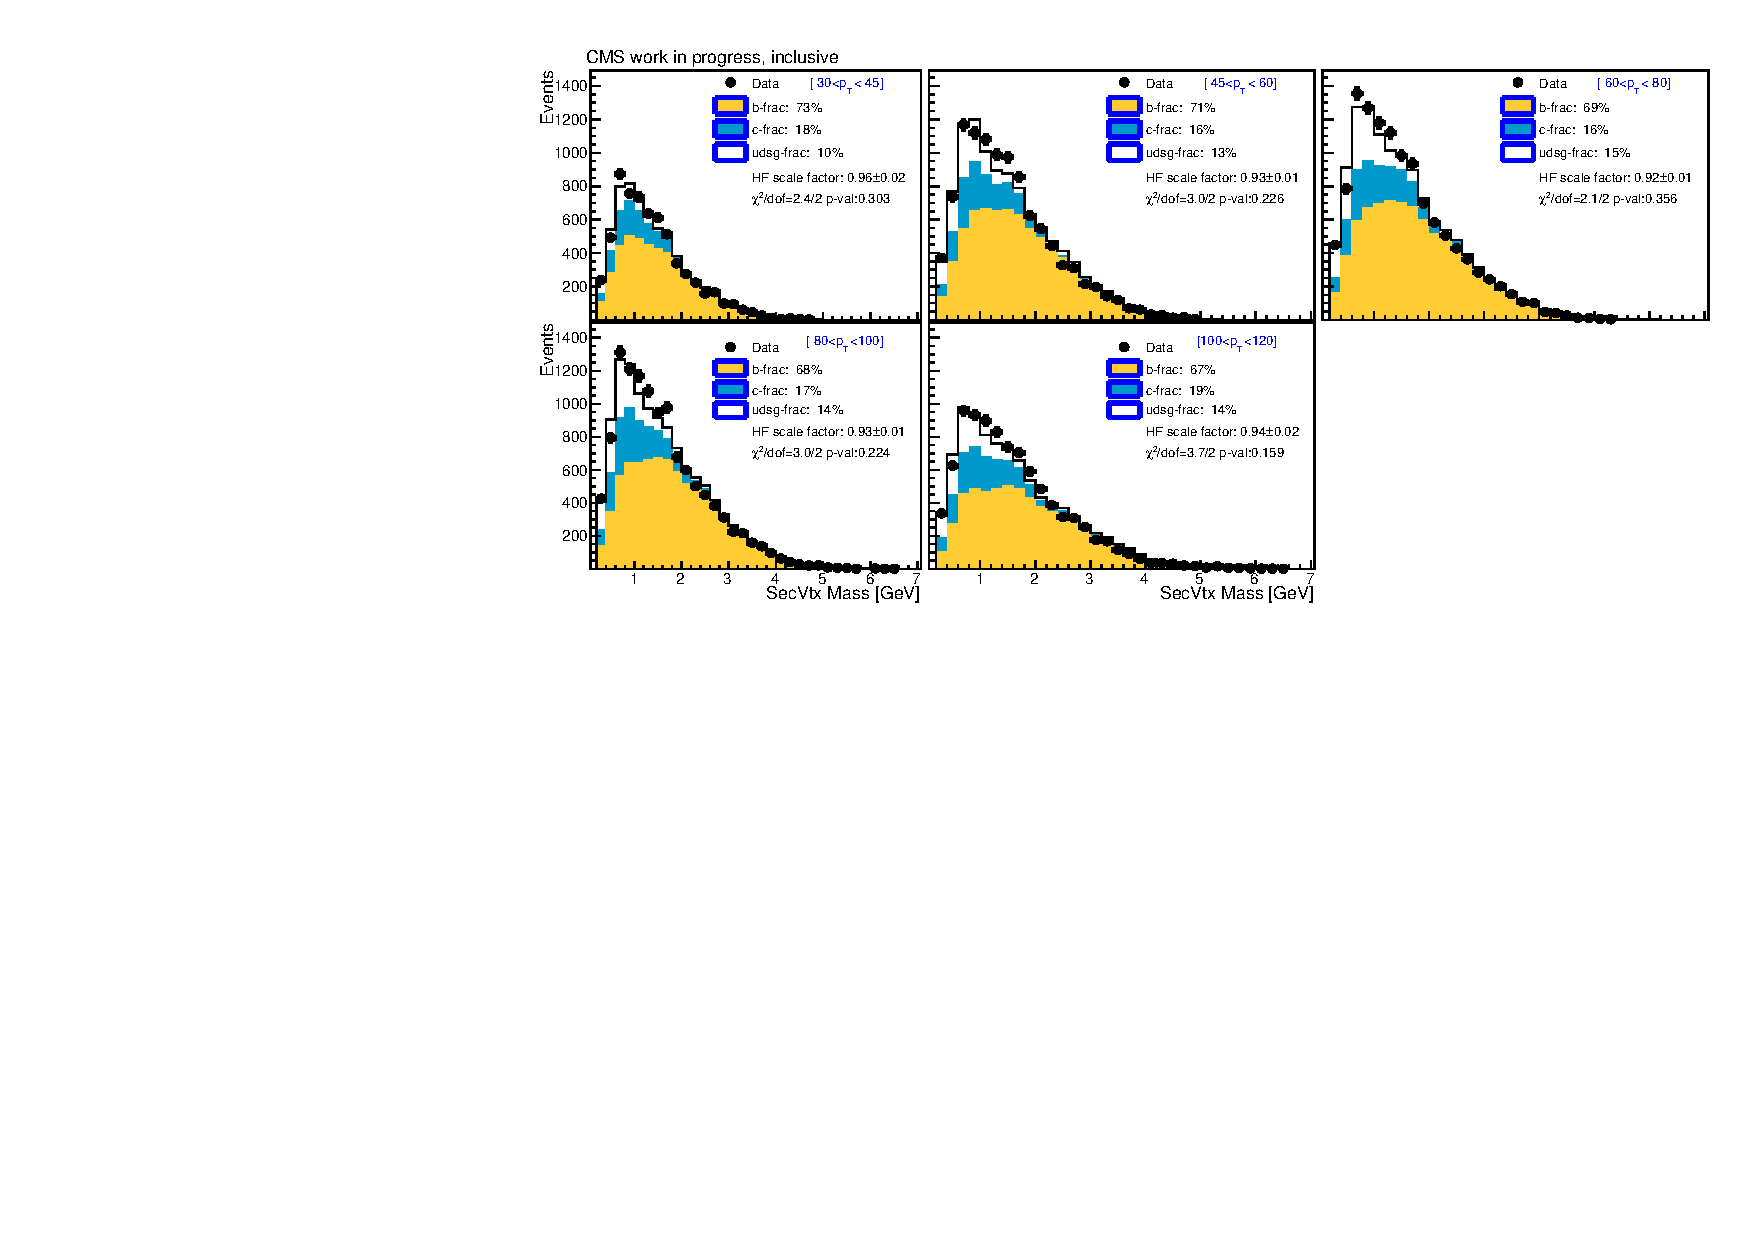
\includegraphics[width=0.8\textwidth]{img/svtx/Multijets__svx}}
\subfloat[][]{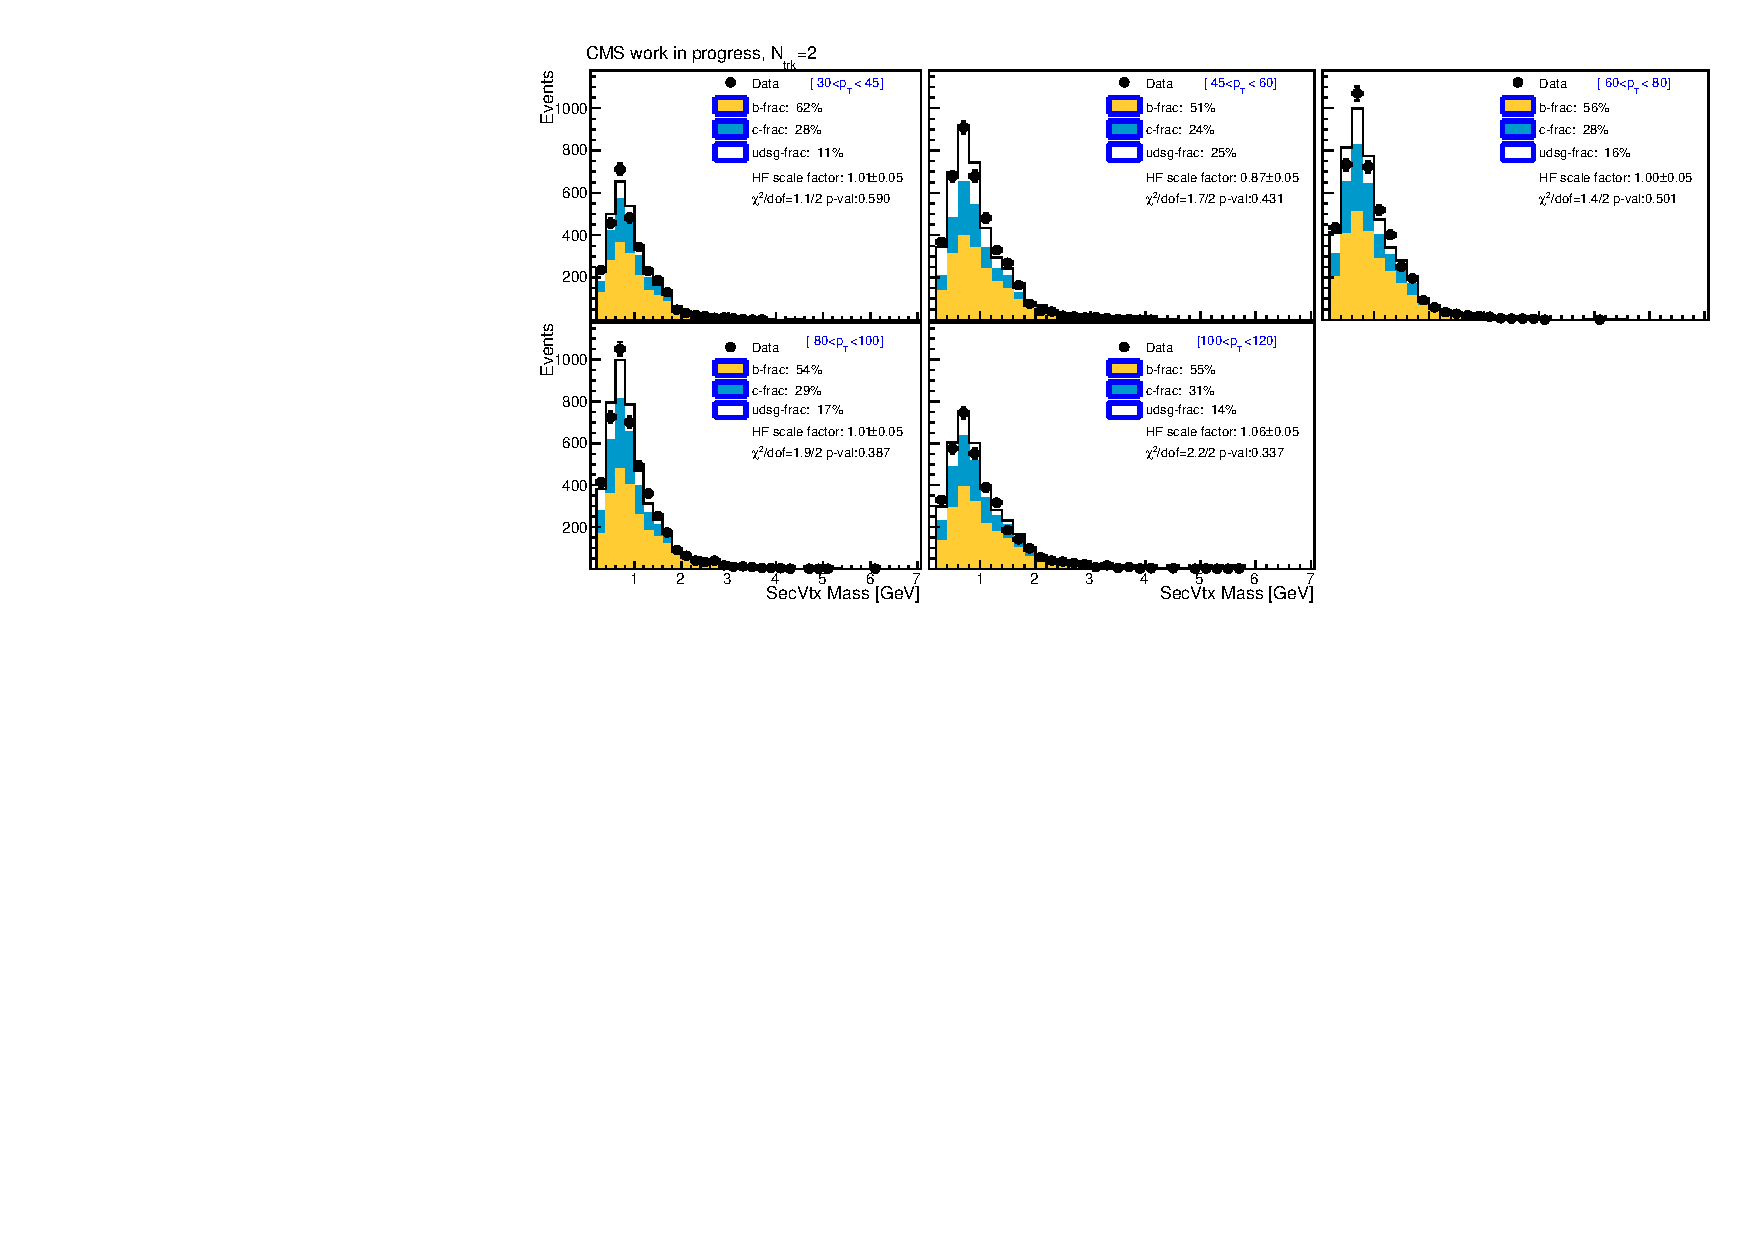
\includegraphics[width=0.8\textwidth]{img/svtx/Multijets_ntrk2_svx}}\\
\subfloat[][]{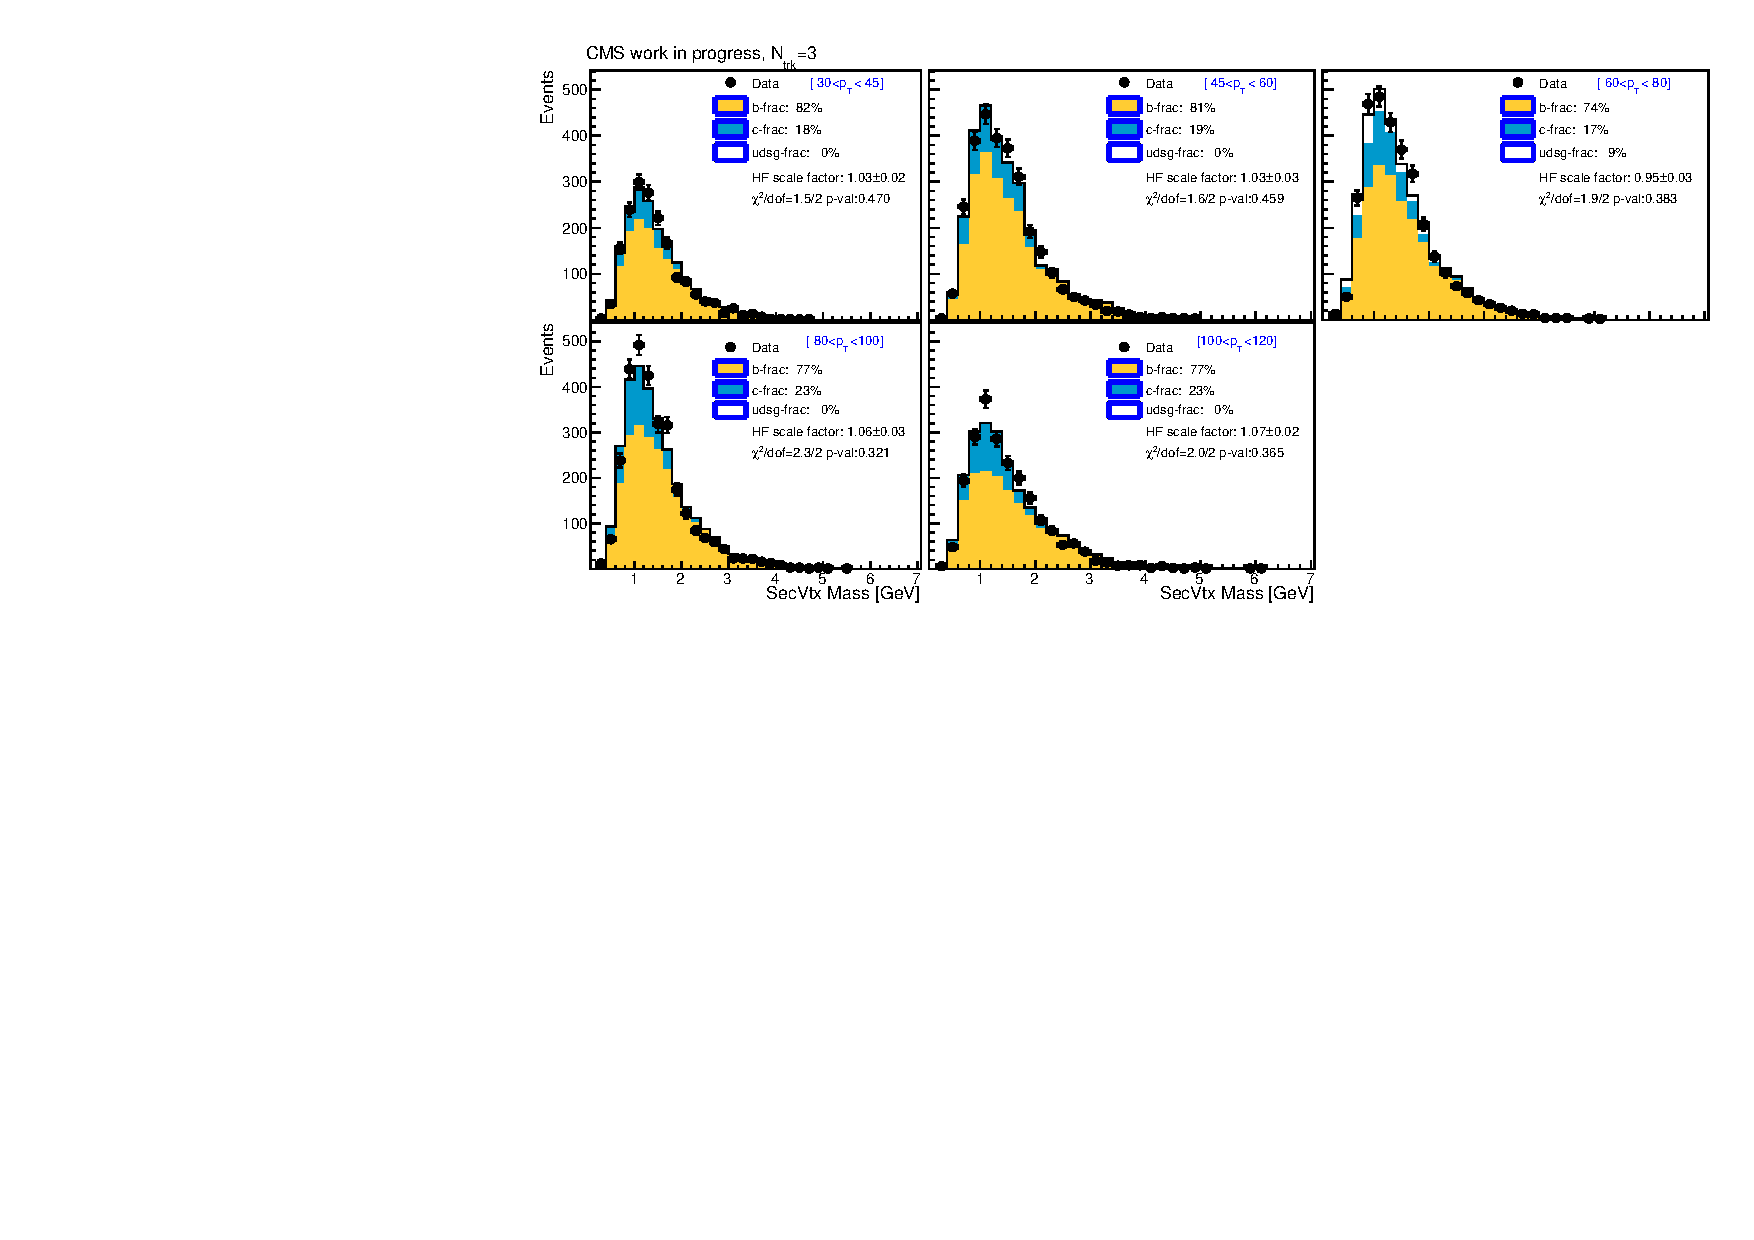
\includegraphics[width=0.8\textwidth]{img/svtx/Multijets_ntrk3_svx}}
\subfloat[][]{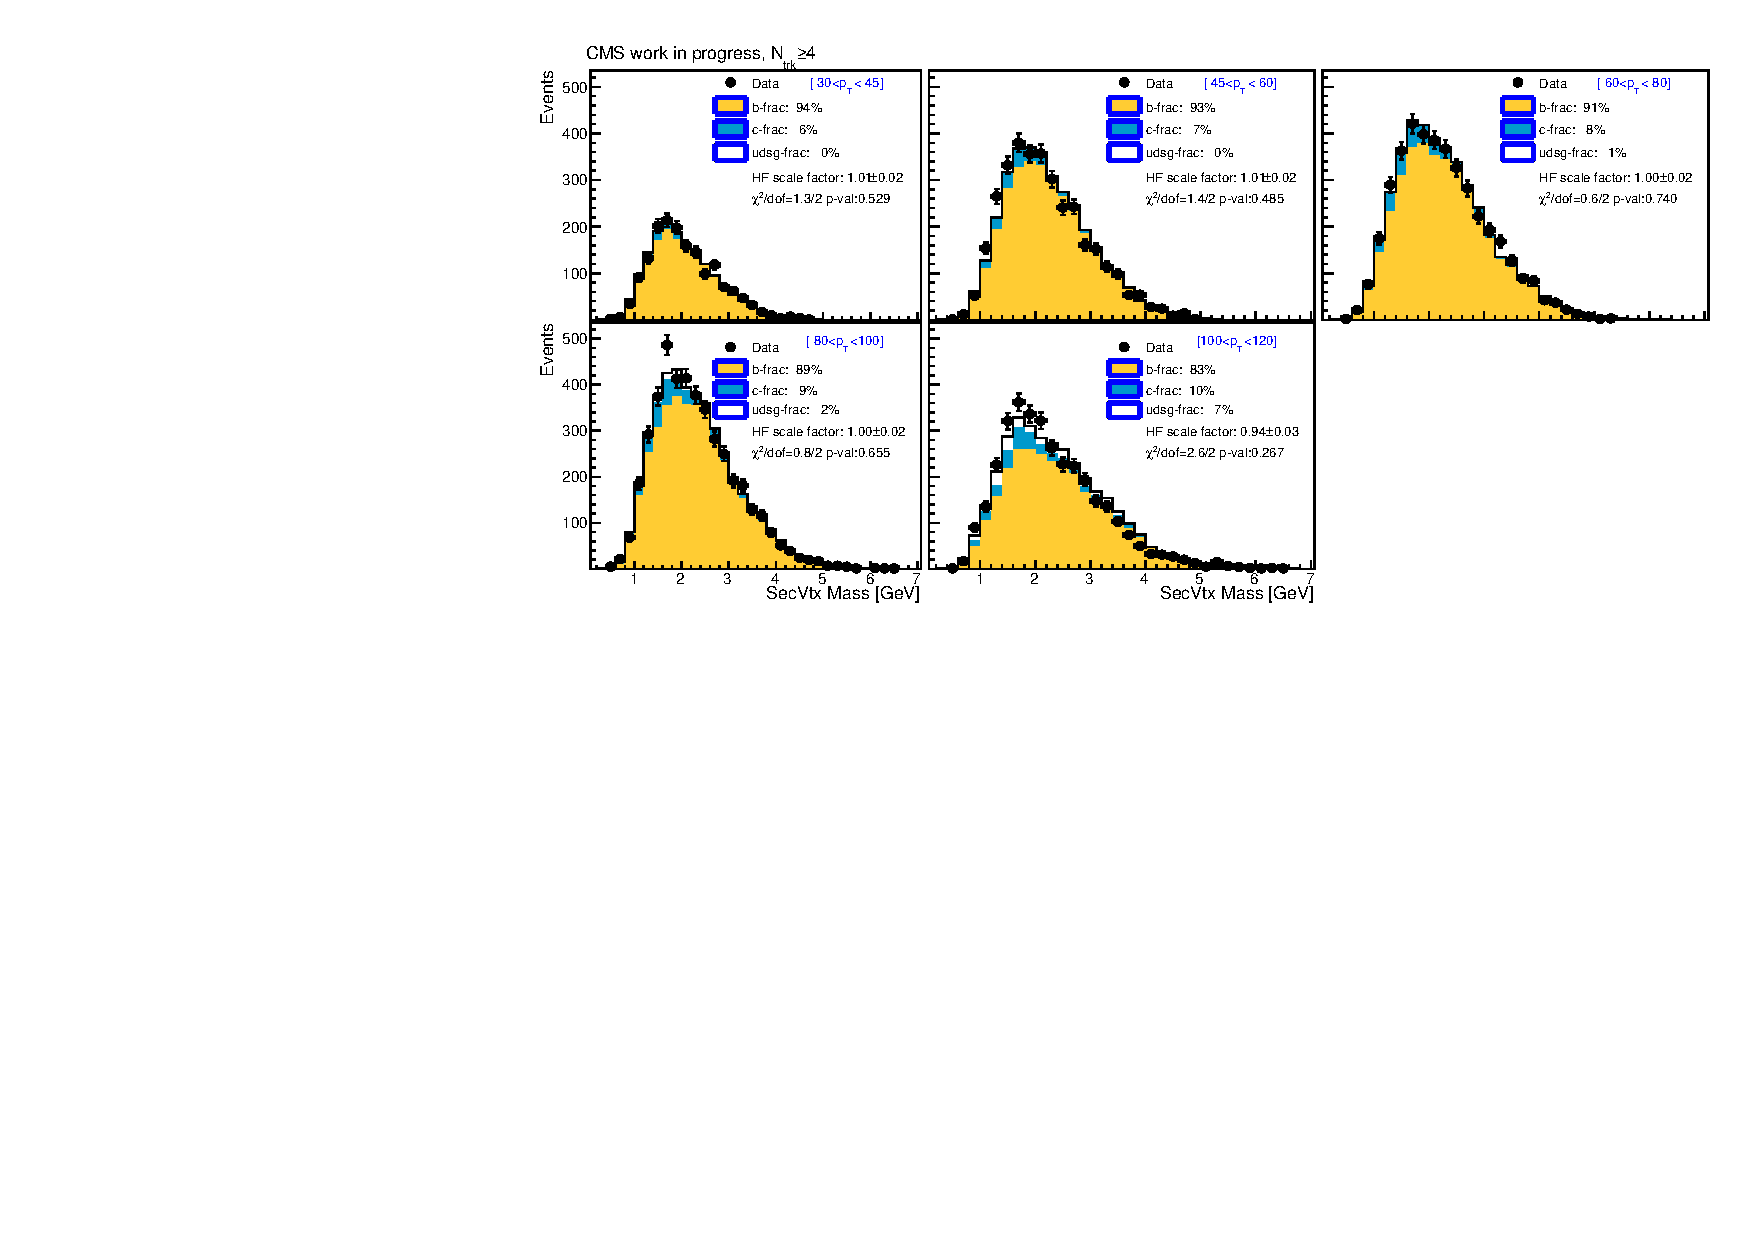
\includegraphics[width=0.8\textwidth]{img/svtx/Multijets_ntrk4_svx}}
\caption{ 
Distribution of the mass of the secondary vertex and expected jet flavour composition after a template fit.
Different jet \pt categories are shown.
The captions show the relative composition of the sample, the common heavy flavour scale factor.
The $\chi^2$ and corresponding probability between data and the result of the fit, are quoted in the captions.
The fits are perfomed to (a) the inclusive secondary vertex spectrum  and to secondary vertices with
(b) 2 tracks, (c) 3 tracks or (d) at least 4 tracks.
}
\label{fig:svtxmass}
\end{figure}
\end{landscape}

\begin{figure}[htp] 
\centering
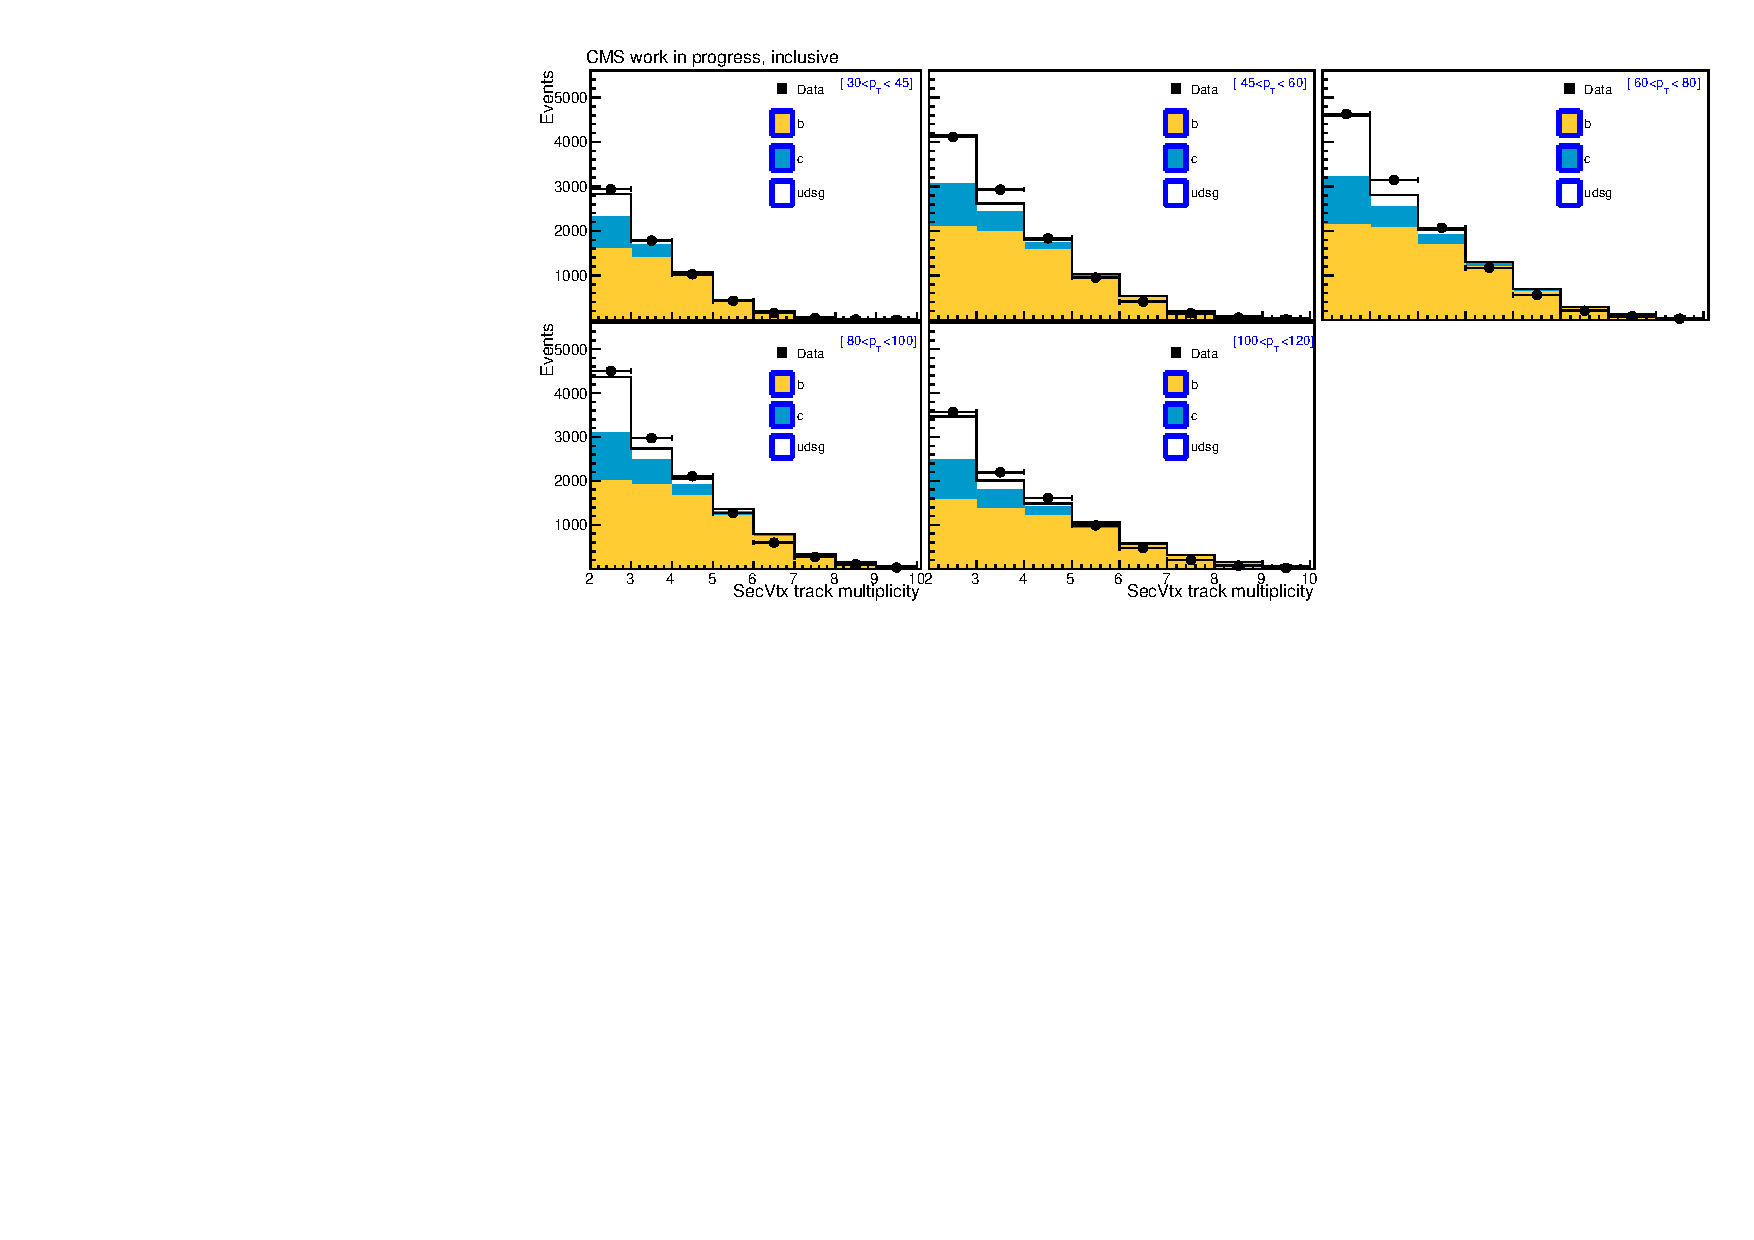
\includegraphics[width=0.9\textwidth]{img/svtx/Multijets__svx_ntracks}
\caption{ 
Distribution of the track multiplcity in secondary vertices. The fraction of each jet flavour reflects the result of the fit to the secondary
vertex mass distribution.}
\label{fig:svtx_trkmult}
\end{figure}


\begin{figure}[htp] 
\centering
\subfloat[][]{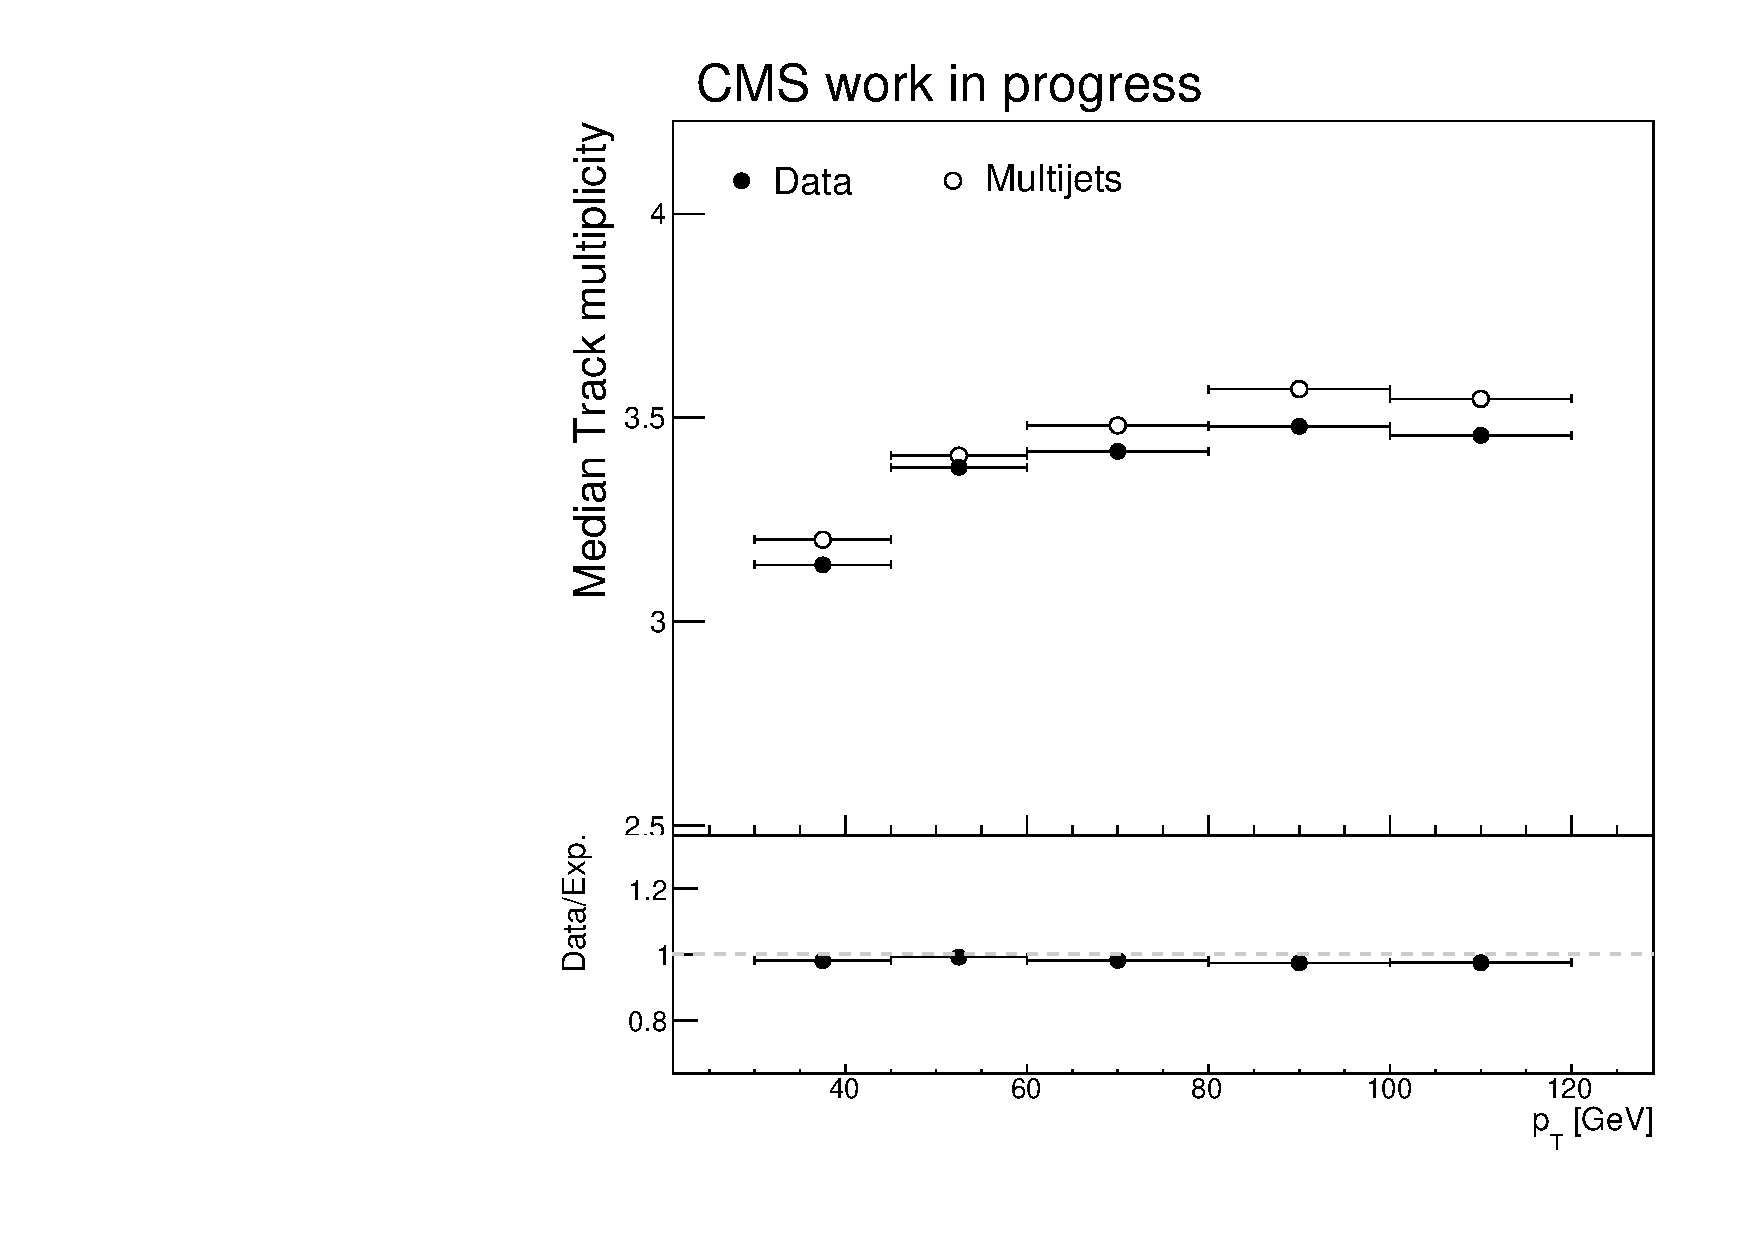
\includegraphics[width=0.49\textwidth]{img/svtx/Multijets__svx_1_ntracks}}
\subfloat[][]{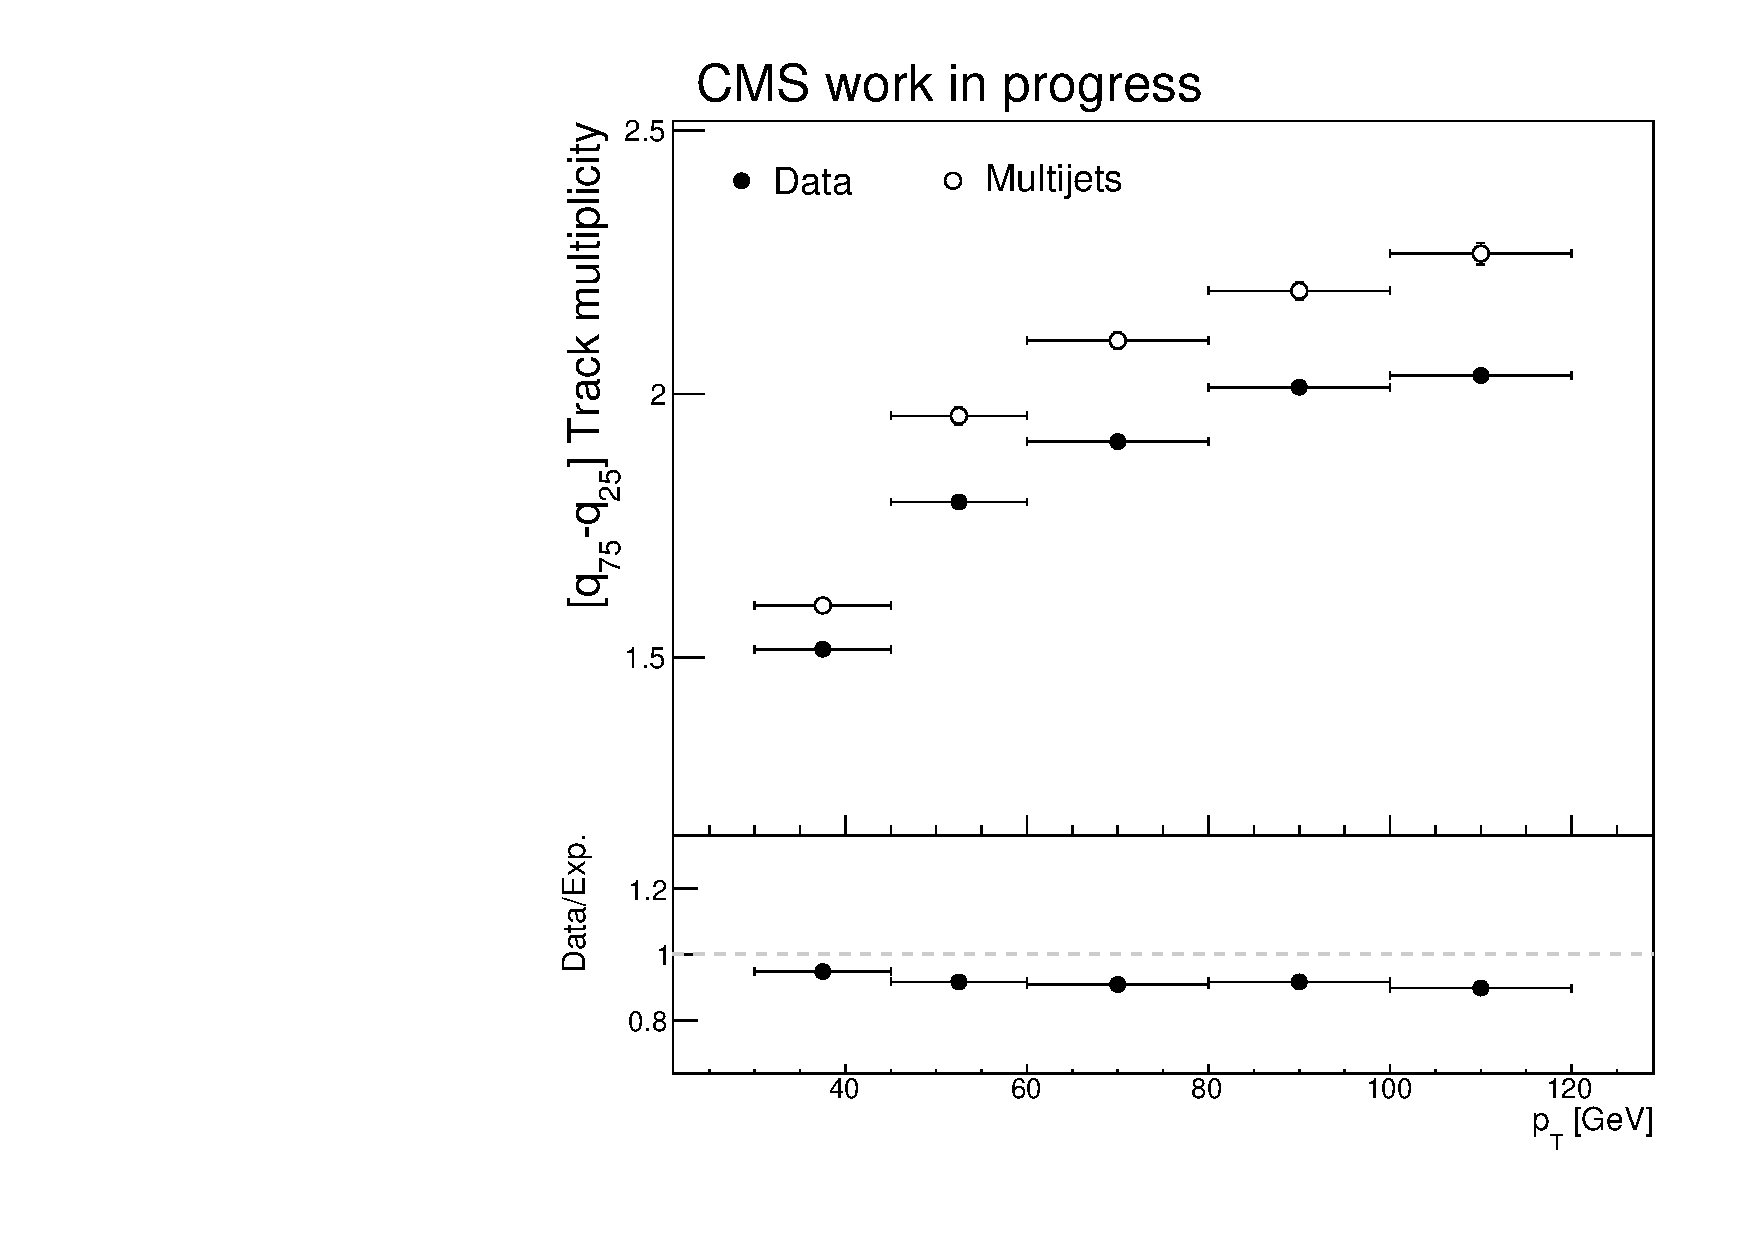
\includegraphics[width=0.49\textwidth]{img/svtx/Multijets__svx_2_ntracks}}
\caption{ 
The (a) median and (b) difference between the 75\% and 25\% quantiles of the track multiplicity distributions for the secondary vertices
are compared between data and the MC (using the fitted jet flavour fractions).
The bottom panels show the data to MC ratio.}
\label{fig:svtx_trkmult_momenta}
\end{figure}

The distributions chosen are the following:

\begin{description}
\item[$L_{\rm xy}$] - the transverse decay length of the secondary vertex, with respect to the primary vertex of the event;
\item[$L_{\rm xy}$ significance] - the ratio between the $L_{\rm xy}$ and its uncertainty;
\item[$\Delta R({\rm SecVtx,jet})$] - the angular distance between the secondary vertex flight direction and the jet axis;
\item[$p_{\rm T}({\rm SecVtx})/\sum p_{\rm T}^{\rm ch}$] - the ratio of the secondary vertex \pt with respect to the scalar sum of the \pt of the charged particles constituting a jet.
\end{description}

For each one, we compute the mean and the difference between the 75\% and 25\% quantiles of both the observed distribution in data
and the expected distribution from simulation. 
The expected distribution is composed using the jet-flavour fractions fit to the SecVtx mass distribution, explained above.
Figures~\ref{fig:svtx_trk2},~\ref{fig:svtx_trk3} and~\ref{fig:svtx_trk4}
show the results obtained for secondary vertices with two, three or at least four associated tracks.
We don't observe significant discrepancies in the chosen variables, 
for the different categories.
The most statistically significant differences found are 
the distribution of the \pt fraction with respect to the  \pt of the charged constituents of the jet
in secondary vertices with two tracks (wider distribution in data)
and in the $L_{\rm xy}$ and $\Delta R$  distributions for 
jets with $\pt>100\GeV$ in secondary vertices with three tracks.
In the first case the diffences seems to come mostly from the quality of the distributions for light jets (udsg),
while in the second case seems related to small statistics in the simulation at high \pt.
Given the general good agreement between data and expectations
in the different track multiplicity categories
we can conclude that there is no severe mismodelling of the performance of the
secondary vertex reconstruction for \cPqb jets.
Thus, the difference in the track multiplicity observed in the inclusive sample can,
be calibrated away with a combination of exclusive measurements.

\begin{landscape}
\begin{figure}[htp] 
\centering
\subfloat[][]{\includegraphics[width=0.34\textwidth]{img/svtx/Multijets_ntrk2_svx_lxy}}
\subfloat[][]{\includegraphics[width=0.34\textwidth]{img/svtx/Multijets_ntrk2_svx_lxysig}}
\subfloat[][]{\includegraphics[width=0.34\textwidth]{img/svtx/Multijets_ntrk2_svx_dr}}
\subfloat[][]{\includegraphics[width=0.34\textwidth]{img/svtx/Multijets_ntrk2_svx_chfrac}}\\
\subfloat[][]{\includegraphics[width=0.34\textwidth]{img/svtx/Multijets_ntrk2_svx_1_lxy}}
\subfloat[][]{\includegraphics[width=0.34\textwidth]{img/svtx/Multijets_ntrk2_svx_1_lxysig}}
\subfloat[][]{\includegraphics[width=0.34\textwidth]{img/svtx/Multijets_ntrk2_svx_1_dr}}
\subfloat[][]{\includegraphics[width=0.34\textwidth]{img/svtx/Multijets_ntrk2_svx_1_chfrac}}\\
\subfloat[][]{\includegraphics[width=0.34\textwidth]{img/svtx/Multijets_ntrk2_svx_2_lxy}}
\subfloat[][]{\includegraphics[width=0.34\textwidth]{img/svtx/Multijets_ntrk2_svx_2_lxysig}}
\subfloat[][]{\includegraphics[width=0.34\textwidth]{img/svtx/Multijets_ntrk2_svx_2_dr}}
\subfloat[][]{\includegraphics[width=0.34\textwidth]{img/svtx/Multijets_ntrk2_svx_2_chfrac}}
\caption{ 
The top plots show different distributions for the properties of secondary vertices with two tracks,
the center plots show the median of the distributions and the
the bottom plots the difference between the 75\% and 25\% quantiles.
(a,e,i) $L_{\rm xy}$,
(b,f,j) $L_{\rm xy}/\sigma_{L_{\rm xy}}$, 
(c,g,k) $\Delta R$, and 
(d,h,l) the ratio of the secondary vertex \pt with respect to the scalar sum of the \pt of the charged constituents of the jet.
The data is compared to the MC (using the fitted jet flavour fractions).
The bottom panels show the data to MC ratio.}
\label{fig:svtx_trk2}
\end{figure}
\end{landscape}

\begin{landscape}
\begin{figure}[htp] 
\centering
\subfloat[][]{\includegraphics[width=0.34\textwidth]{img/svtx/Multijets_ntrk3_svx_lxy}}
\subfloat[][]{\includegraphics[width=0.34\textwidth]{img/svtx/Multijets_ntrk3_svx_lxysig}}
\subfloat[][]{\includegraphics[width=0.34\textwidth]{img/svtx/Multijets_ntrk3_svx_dr}}
\subfloat[][]{\includegraphics[width=0.34\textwidth]{img/svtx/Multijets_ntrk3_svx_chfrac}}\\
\subfloat[][]{\includegraphics[width=0.34\textwidth]{img/svtx/Multijets_ntrk3_svx_1_lxy}}
\subfloat[][]{\includegraphics[width=0.34\textwidth]{img/svtx/Multijets_ntrk3_svx_1_lxysig}}
\subfloat[][]{\includegraphics[width=0.34\textwidth]{img/svtx/Multijets_ntrk3_svx_1_dr}}
\subfloat[][]{\includegraphics[width=0.34\textwidth]{img/svtx/Multijets_ntrk3_svx_1_chfrac}}\\
\subfloat[][]{\includegraphics[width=0.34\textwidth]{img/svtx/Multijets_ntrk3_svx_2_lxy}}
\subfloat[][]{\includegraphics[width=0.34\textwidth]{img/svtx/Multijets_ntrk3_svx_2_lxysig}}
\subfloat[][]{\includegraphics[width=0.34\textwidth]{img/svtx/Multijets_ntrk3_svx_2_dr}}
\subfloat[][]{\includegraphics[width=0.34\textwidth]{img/svtx/Multijets_ntrk3_svx_2_chfrac}}
\caption{ 
Similar to Fig.~\ref{fig:svtx_trk2} but for secondary vertices with three tracks.}
\label{fig:svtx_trk3}
\end{figure}
\end{landscape}

\begin{landscape}
\begin{figure}[htp] 
\centering
\subfloat[][]{\includegraphics[width=0.34\textwidth]{img/svtx/Multijets_ntrk4_svx_lxy}}
\subfloat[][]{\includegraphics[width=0.34\textwidth]{img/svtx/Multijets_ntrk4_svx_lxysig}}
\subfloat[][]{\includegraphics[width=0.34\textwidth]{img/svtx/Multijets_ntrk4_svx_dr}}
\subfloat[][]{\includegraphics[width=0.34\textwidth]{img/svtx/Multijets_ntrk4_svx_chfrac}}\\
\subfloat[][]{\includegraphics[width=0.34\textwidth]{img/svtx/Multijets_ntrk4_svx_1_lxy}}
\subfloat[][]{\includegraphics[width=0.34\textwidth]{img/svtx/Multijets_ntrk4_svx_1_lxysig}}
\subfloat[][]{\includegraphics[width=0.34\textwidth]{img/svtx/Multijets_ntrk4_svx_1_dr}}
\subfloat[][]{\includegraphics[width=0.34\textwidth]{img/svtx/Multijets_ntrk4_svx_1_chfrac}}\\
\subfloat[][]{\includegraphics[width=0.34\textwidth]{img/svtx/Multijets_ntrk4_svx_2_lxy}}
\subfloat[][]{\includegraphics[width=0.34\textwidth]{img/svtx/Multijets_ntrk4_svx_2_lxysig}}
\subfloat[][]{\includegraphics[width=0.34\textwidth]{img/svtx/Multijets_ntrk4_svx_2_dr}}
\subfloat[][]{\includegraphics[width=0.34\textwidth]{img/svtx/Multijets_ntrk4_svx_2_chfrac}}
\caption{ 
Similar to Fig.~\ref{fig:svtx_trk2} but for secondary vertices with at least four tracks.}
\label{fig:svtx_trk4}
\end{figure}
\end{landscape}


%
%
%
\clearpage
\section{Measuring the top quark mass using tracks and vertices}
\label{sec:mtoptkvtx}

\subsection{Strategy}
\label{subsec:strategy}

\subsection{Signal, background and fitting models}
\label{subsec:models}

\subsection{Calibration}
\label{subsec:calibration}

\subsection{Systematic uncertainties}
\label{subsec:syst}

\subsection{Results}
\label{subsec:results}


%
%
%
\clearpage
\section{Summary}
\label{sec:summary}

Coming soon.



\clearpage
\bibliography{auto_generated}   % will be created by the tdr script.


%%% DO NOT ADD \end{document}!

